\documentclass[twoside]{book}

% Packages required by doxygen
\usepackage{fixltx2e}
\usepackage{calc}
\usepackage{doxygen}
\usepackage[export]{adjustbox} % also loads graphicx
\usepackage{graphicx}
\usepackage[utf8]{inputenc}
\usepackage{makeidx}
\usepackage{multicol}
\usepackage{multirow}
\PassOptionsToPackage{warn}{textcomp}
\usepackage{textcomp}
\usepackage[nointegrals]{wasysym}
\usepackage[table]{xcolor}

% Font selection
\usepackage[T1]{fontenc}
\usepackage[scaled=.90]{helvet}
\usepackage{courier}
\usepackage{amssymb}
\usepackage{sectsty}
\renewcommand{\familydefault}{\sfdefault}
\allsectionsfont{%
  \fontseries{bc}\selectfont%
  \color{darkgray}%
}
\renewcommand{\DoxyLabelFont}{%
  \fontseries{bc}\selectfont%
  \color{darkgray}%
}
\newcommand{\+}{\discretionary{\mbox{\scriptsize$\hookleftarrow$}}{}{}}

% Page & text layout
\usepackage{geometry}
\geometry{%
  a4paper,%
  top=2.5cm,%
  bottom=2.5cm,%
  left=2.5cm,%
  right=2.5cm%
}
\tolerance=750
\hfuzz=15pt
\hbadness=750
\setlength{\emergencystretch}{15pt}
\setlength{\parindent}{0cm}
\setlength{\parskip}{3ex plus 2ex minus 2ex}
\makeatletter
\renewcommand{\paragraph}{%
  \@startsection{paragraph}{4}{0ex}{-1.0ex}{1.0ex}{%
    \normalfont\normalsize\bfseries\SS@parafont%
  }%
}
\renewcommand{\subparagraph}{%
  \@startsection{subparagraph}{5}{0ex}{-1.0ex}{1.0ex}{%
    \normalfont\normalsize\bfseries\SS@subparafont%
  }%
}
\makeatother

% Headers & footers
\usepackage{fancyhdr}
\pagestyle{fancyplain}
\fancyhead[LE]{\fancyplain{}{\bfseries\thepage}}
\fancyhead[CE]{\fancyplain{}{}}
\fancyhead[RE]{\fancyplain{}{\bfseries\leftmark}}
\fancyhead[LO]{\fancyplain{}{\bfseries\rightmark}}
\fancyhead[CO]{\fancyplain{}{}}
\fancyhead[RO]{\fancyplain{}{\bfseries\thepage}}
\fancyfoot[LE]{\fancyplain{}{}}
\fancyfoot[CE]{\fancyplain{}{}}
\fancyfoot[RE]{\fancyplain{}{\bfseries\scriptsize Generated by Doxygen }}
\fancyfoot[LO]{\fancyplain{}{\bfseries\scriptsize Generated by Doxygen }}
\fancyfoot[CO]{\fancyplain{}{}}
\fancyfoot[RO]{\fancyplain{}{}}
\renewcommand{\footrulewidth}{0.4pt}
\renewcommand{\chaptermark}[1]{%
  \markboth{#1}{}%
}
\renewcommand{\sectionmark}[1]{%
  \markright{\thesection\ #1}%
}

% Indices & bibliography
\usepackage{natbib}
\usepackage[titles]{tocloft}
\setcounter{tocdepth}{3}
\setcounter{secnumdepth}{5}
\makeindex

% Hyperlinks (required, but should be loaded last)
\usepackage{ifpdf}
\ifpdf
  \usepackage[pdftex,pagebackref=true]{hyperref}
\else
  \usepackage[ps2pdf,pagebackref=true]{hyperref}
\fi
\hypersetup{%
  colorlinks=true,%
  linkcolor=blue,%
  citecolor=blue,%
  unicode%
}

% Custom commands
\newcommand{\clearemptydoublepage}{%
  \newpage{\pagestyle{empty}\cleardoublepage}%
}

\usepackage{caption}
\captionsetup{labelsep=space,justification=centering,font={bf},singlelinecheck=off,skip=4pt,position=top}

%===== C O N T E N T S =====

\begin{document}

% Titlepage & ToC
\hypersetup{pageanchor=false,
             bookmarksnumbered=true,
             pdfencoding=unicode
            }
\pagenumbering{alph}
\begin{titlepage}
\vspace*{7cm}
\begin{center}%
{\Large M\+\_\+escape }\\
\vspace*{1cm}
{\large Generated by Doxygen 1.8.14}\\
\end{center}
\end{titlepage}
\clearemptydoublepage
\pagenumbering{roman}
\tableofcontents
\clearemptydoublepage
\pagenumbering{arabic}
\hypersetup{pageanchor=true}

%--- Begin generated contents ---
\chapter{M\+\_\+escape Fortran Library}
\label{index}\hypertarget{index}{}    

    \hypertarget{index_Introduction}{}\section{Introduction}\label{index_Introduction}
A\+N\+SI terminal escape sequences

      
\chapter{Modules Index}
\section{Modules List}
Here is a list of all modules with brief descriptions\+:\begin{DoxyCompactList}
\item\contentsline{section}{\mbox{\hyperlink{namespacem__escape}{m\+\_\+escape}} \\*\subsubsection*{N\+A\+ME}

M\+\_\+escape(3f) -\/ \mbox{[}M\+\_\+escape\mbox{]} substitute escape sequences for X\+M\+L-\/like syntax in strings }{\pageref{namespacem__escape}}{}
\item\contentsline{section}{\mbox{\hyperlink{namespacem__list}{m\+\_\+list}} \\*\subsubsection*{N\+A\+ME}

M\+\_\+list(3f) -\/ \mbox{[}M\+\_\+list\mbox{]} maintain simple lists (L\+I\+C\+E\+N\+SE\+:PD) }{\pageref{namespacem__list}}{}
\end{DoxyCompactList}

\chapter{Data Type Index}
\doxysection{Data Types List}
Here are the data types with brief descriptions\+:\begin{DoxyCompactList}
\item\contentsline{section}{\mbox{\hyperlink{structm__list2_1_1dictionary}{m\+\_\+list2\+::dictionary}} }{\pageref{structm__list2_1_1dictionary}}{}
\item\contentsline{section}{\mbox{\hyperlink{interfacem__list2_1_1insert}{m\+\_\+list2\+::insert}} }{\pageref{interfacem__list2_1_1insert}}{}
\item\contentsline{section}{\mbox{\hyperlink{interfacem__list2_1_1locate}{m\+\_\+list2\+::locate}} }{\pageref{interfacem__list2_1_1locate}}{}
\item\contentsline{section}{\mbox{\hyperlink{interfacem__list2_1_1remove}{m\+\_\+list2\+::remove}} }{\pageref{interfacem__list2_1_1remove}}{}
\item\contentsline{section}{\mbox{\hyperlink{interfacem__list2_1_1replace}{m\+\_\+list2\+::replace}} }{\pageref{interfacem__list2_1_1replace}}{}
\end{DoxyCompactList}

\chapter{File Index}
\doxysection{File List}
Here is a list of all files with brief descriptions\+:\begin{DoxyCompactList}
\item\contentsline{section}{/home/urbanjs/venus/\+V600/github/\+M\+\_\+escape/src/\mbox{\hyperlink{M__escape_8f90}{M\+\_\+escape.\+f90}} }{\pageref{M__escape_8f90}}{}
\item\contentsline{section}{/home/urbanjs/venus/\+V600/github/\+M\+\_\+escape/src/\mbox{\hyperlink{M__list2_8f90}{M\+\_\+list2.\+f90}} }{\pageref{M__list2_8f90}}{}
\end{DoxyCompactList}

\chapter{Module Documentation}
\hypertarget{namespacem__escape}{}\section{m\+\_\+escape Module Reference}
\label{namespacem__escape}\index{m\+\_\+escape@{m\+\_\+escape}}


\subsubsection*{N\+A\+ME}

M\+\_\+escape(3f) -\/ \mbox{[}M\+\_\+escape\mbox{]} substitute escape sequences for X\+M\+L-\/like syntax in strings  


\subsection*{Functions/\+Subroutines}
\begin{DoxyCompactItemize}
\item 
character(len=\+:) function, allocatable, public \mbox{\hyperlink{namespacem__escape_a36f016baad6b23f86189e6f3ee6db0cb}{esc}} (string, clear\+\_\+at\+\_\+end)
\begin{DoxyCompactList}\small\item\em \subsubsection*{N\+A\+ME}

esc(3f) -\/ \mbox{[}M\+\_\+escape\mbox{]} substitute escape sequences for X\+M\+L-\/like syntax in strings \end{DoxyCompactList}\item 
character(len=\+:) function, allocatable, public \mbox{\hyperlink{namespacem__escape_af7d28a73e65efb58beeb684d7bdeefec}{color}} (string, fg, bg, style)
\begin{DoxyCompactList}\small\item\em \subsubsection*{N\+A\+ME}

color(3f) -\/ \mbox{[}M\+\_\+escape\mbox{]} colorize text using a simple function-\/based approach (L\+I\+C\+E\+N\+SE\+:PD) \subsubsection*{S\+Y\+N\+O\+P\+S\+IS}\end{DoxyCompactList}\item 
subroutine, public \mbox{\hyperlink{namespacem__escape_a24566737cb6aa1672180eaa21c8d4f66}{color\+\_\+mode}} (switch)
\begin{DoxyCompactList}\small\item\em \subsubsection*{N\+A\+ME}

color\+\_\+mode(3f) -\/ \mbox{[}M\+\_\+escape\mbox{]} toggle style effects of color(3f) on and off (L\+I\+C\+E\+N\+SE\+:PD) \subsubsection*{S\+Y\+N\+O\+P\+S\+IS}\end{DoxyCompactList}\item 
subroutine \mbox{\hyperlink{namespacem__escape_ae9d40717b2e75e90e2505d5fed6435c5}{vt102}} ()
\item 
subroutine, public \mbox{\hyperlink{namespacem__escape_a4210456d81d9a1bf328093a9635e640b}{esc\+\_\+mode}} (manner)
\begin{DoxyCompactList}\small\item\em \subsubsection*{N\+A\+ME}

esc\+\_\+mode(3f) -\/ \mbox{[}M\+\_\+escape\mbox{]} select processing mode for output from esc(3f) \subsubsection*{S\+Y\+N\+O\+P\+S\+IS}\end{DoxyCompactList}\item 
subroutine \mbox{\hyperlink{namespacem__escape_a1bc574bc97157fe67d868d2bd180c91e}{wipe\+\_\+dictionary}} ()
\item 
subroutine, public \mbox{\hyperlink{namespacem__escape_a5efd612f60d281003917329484a7960c}{update}} (key, valin)
\begin{DoxyCompactList}\small\item\em \subsubsection*{N\+A\+ME}

update(3f) -\/ \mbox{[}M\+\_\+escape\mbox{]} update internal dictionary given keyword and value (L\+I\+C\+E\+N\+SE\+:PD) \subsubsection*{S\+Y\+N\+O\+P\+S\+IS}\end{DoxyCompactList}\item 
character(len=\+:) function, allocatable \mbox{\hyperlink{namespacem__escape_af555c90c278ff964d8bce93ee0368a42}{get}} (key)
\item 
subroutine, public \mbox{\hyperlink{namespacem__escape_a6add907828fd34e94b87f643a5cabc64}{print\+\_\+dictionary}} (header)
\begin{DoxyCompactList}\small\item\em \subsubsection*{N\+A\+ME}

print\+\_\+dictionary(3f) -\/ \mbox{[}A\+R\+G\+U\+M\+E\+N\+TS\+:M\+\_\+\+C\+L\+I2\mbox{]} print internal dictionary created by calls to update(3f) (L\+I\+C\+E\+N\+SE\+:PD) \subsubsection*{S\+Y\+N\+O\+P\+S\+IS}\end{DoxyCompactList}\item 
subroutine \mbox{\hyperlink{namespacem__escape_af23bd97702864e0f32258e6ec0d51506}{split}} (input\+\_\+line, array, delimiters)
\item 
character(len=\+:) function, allocatable, public \mbox{\hyperlink{namespacem__escape_a916b16ce9be553d669f54cb9575a91be}{attr}} (attribute, text)
\begin{DoxyCompactList}\small\item\em \subsubsection*{N\+A\+ME}

attr(3f) -\/ \mbox{[}M\+\_\+escape\mbox{]} colorize text using a simple function-\/based approach (L\+I\+C\+E\+N\+SE\+:PD) \subsubsection*{S\+Y\+N\+O\+P\+S\+IS}\end{DoxyCompactList}\end{DoxyCompactItemize}
\subsection*{Variables}
\begin{DoxyCompactItemize}
\item 
logical, save \mbox{\hyperlink{namespacem__escape_a67ff4e5b90da8436f0da5882c4a5720c}{g\+\_\+color}} =.true.
\item 
logical, save \mbox{\hyperlink{namespacem__escape_af068eb2561159352a9a406c95157b131}{debug}} =.false.
\item 
character(len=\+:), dimension(\+:), allocatable, save \mbox{\hyperlink{namespacem__escape_a35e957e007844dbfe641b3d915fba048}{keywords}}
\item 
character(len=\+:), dimension(\+:), allocatable, save \mbox{\hyperlink{namespacem__escape_a4c3b430bde66148e6f2c79c5418384fa}{values}}
\item 
integer, dimension(\+:), allocatable, save \mbox{\hyperlink{namespacem__escape_a7e8e011813de1e58d7c8bcda489d8f1c}{counts}}
\item 
character(len=\+:), allocatable, save \mbox{\hyperlink{namespacem__escape_ab4e7fcb41457772a9bd4e4413d5355d6}{mode}}
\item 
character(len= $\ast$), parameter \mbox{\hyperlink{namespacem__escape_aa17be0f87e5ec9012a38c04bfbb5e588}{nl}} =new\+\_\+line(\textquotesingle{}a\textquotesingle{})
\item 
character(len= $\ast$), parameter \mbox{\hyperlink{namespacem__escape_a9931f535eb0f6f24df5a121331faa5ef}{escape}} =achar(27) \textbackslash{}\char`\"{}
\item 
character(len= $\ast$), parameter \mbox{\hyperlink{namespacem__escape_a6d5af6b1571cba22511523c53c71fa6f}{code\+\_\+start}} =E\+S\+C\+A\+PE//\textquotesingle{}\mbox{[}\textquotesingle{}
\item 
character(len= $\ast$), parameter \mbox{\hyperlink{namespacem__escape_af913c326395b9bf2c089c30698d2c742}{code\+\_\+end}} =\textquotesingle{}m\textquotesingle{}
\item 
character(len= $\ast$), parameter \mbox{\hyperlink{namespacem__escape_aaaf7224f2104dcd571cdaa69b61b9d01}{code\+\_\+reset}} =C\+O\+D\+E\+\_\+\+S\+T\+A\+RT//\textquotesingle{}0\textquotesingle{}//C\+O\+D\+E\+\_\+\+E\+ND
\item 
character(len= $\ast$), parameter \mbox{\hyperlink{namespacem__escape_a9d45e30ea5891b89dc9a61ba1b5dbc03}{clear\+\_\+display}} =C\+O\+D\+E\+\_\+\+S\+T\+A\+RT//\textquotesingle{}2\+J\textquotesingle{}
\item 
character(len= $\ast$), parameter \mbox{\hyperlink{namespacem__escape_ae4634ac062742627f215df29998fc677}{home\+\_\+display}} =C\+O\+D\+E\+\_\+\+S\+T\+A\+RT//\textquotesingle{}H\textquotesingle{}
\item 
character(len= $\ast$), parameter \mbox{\hyperlink{namespacem__escape_a2cd9c30d3783af9d1f74a50e7f1dbd7f}{bell}} =achar(7)
\item 
character(len= $\ast$), parameter \mbox{\hyperlink{namespacem__escape_a8f30470c66af08cf881d9afe23357a03}{bold\+\_\+on}} =\textquotesingle{}1\textquotesingle{}
\item 
character(len= $\ast$), parameter \mbox{\hyperlink{namespacem__escape_a5bd07ea0cedbfd7d0e04b3b0be74821f}{italic\+\_\+on}} =\textquotesingle{}3\textquotesingle{}
\item 
character(len= $\ast$), parameter \mbox{\hyperlink{namespacem__escape_a6f4bcc5f8acb0683ed6d8e05c0100daa}{underline\+\_\+on}} =\textquotesingle{}4\textquotesingle{}
\item 
character(len= $\ast$), parameter \mbox{\hyperlink{namespacem__escape_afacdc9d33171b768ee026b1eb6726f8a}{inverse\+\_\+on}} =\textquotesingle{}7\textquotesingle{}
\item 
character(len= $\ast$), parameter \mbox{\hyperlink{namespacem__escape_a978fe9a5d07621c57c3163d8a7a62118}{bold\+\_\+off}} =\textquotesingle{}22\textquotesingle{}
\item 
character(len= $\ast$), parameter \mbox{\hyperlink{namespacem__escape_a93fc5a4e6f0ed044c9f6cf29412a05cb}{italic\+\_\+off}} =\textquotesingle{}23\textquotesingle{}
\item 
character(len= $\ast$), parameter \mbox{\hyperlink{namespacem__escape_a9e36a1a9bd4a64702ecef4a2e3d592b9}{underline\+\_\+off}} =\textquotesingle{}24\textquotesingle{}
\item 
character(len= $\ast$), parameter \mbox{\hyperlink{namespacem__escape_affae80c7d63858227a9f3134e6191f96}{inverse\+\_\+off}} =\textquotesingle{}27\textquotesingle{}
\item 
character(len= $\ast$), parameter \mbox{\hyperlink{namespacem__escape_a6c7b72b2cfc0a6ec7fc4080ad6750d99}{color\+\_\+fg\+\_\+black}} =\textquotesingle{}30\textquotesingle{}
\item 
character(len= $\ast$), parameter \mbox{\hyperlink{namespacem__escape_a35eecf0fb916821d94b9c47b2045fe44}{color\+\_\+fg\+\_\+red}} =\textquotesingle{}31\textquotesingle{}
\item 
character(len= $\ast$), parameter \mbox{\hyperlink{namespacem__escape_aeab9b03c1de2c6fb13031c9ca55f9105}{color\+\_\+fg\+\_\+green}} =\textquotesingle{}32\textquotesingle{}
\item 
character(len= $\ast$), parameter \mbox{\hyperlink{namespacem__escape_accc5b67f05d8a2b02ca6f4a0ba38e581}{color\+\_\+fg\+\_\+yellow}} =\textquotesingle{}33\textquotesingle{}
\item 
character(len= $\ast$), parameter \mbox{\hyperlink{namespacem__escape_a01075e619c6af06aac80d73f32263439}{color\+\_\+fg\+\_\+blue}} =\textquotesingle{}34\textquotesingle{}
\item 
character(len= $\ast$), parameter \mbox{\hyperlink{namespacem__escape_ac56b264a4d6c5f3668bac32b791e54de}{color\+\_\+fg\+\_\+magenta}} =\textquotesingle{}35\textquotesingle{}
\item 
character(len= $\ast$), parameter \mbox{\hyperlink{namespacem__escape_a0bbc85c7110c9b67456884baafe31daf}{color\+\_\+fg\+\_\+cyan}} =\textquotesingle{}36\textquotesingle{}
\item 
character(len= $\ast$), parameter \mbox{\hyperlink{namespacem__escape_ae410339e5c6b5468a65e8ce193941ea4}{color\+\_\+fg\+\_\+white}} =\textquotesingle{}37\textquotesingle{}
\item 
character(len= $\ast$), parameter \mbox{\hyperlink{namespacem__escape_aaeff9968bb1e29198469d5d8109e5f41}{color\+\_\+fg\+\_\+default}} =\textquotesingle{}39\textquotesingle{}
\item 
character(len= $\ast$), parameter \mbox{\hyperlink{namespacem__escape_a75d8856bae4a4b8875d48ce2e3a3409a}{color\+\_\+fg\+\_\+black\+\_\+intense}} =\textquotesingle{}90\textquotesingle{}
\item 
character(len= $\ast$), parameter \mbox{\hyperlink{namespacem__escape_a9355532fa2ee17b47e72208480a86707}{color\+\_\+fg\+\_\+red\+\_\+intense}} =\textquotesingle{}91\textquotesingle{}
\item 
character(len= $\ast$), parameter \mbox{\hyperlink{namespacem__escape_a21c7f9b0377ba62dc353e09c05cc5f35}{color\+\_\+fg\+\_\+green\+\_\+intense}} =\textquotesingle{}92\textquotesingle{}
\item 
character(len= $\ast$), parameter \mbox{\hyperlink{namespacem__escape_a7fb2b231cf28bd2ffbf015d7430b46db}{color\+\_\+fg\+\_\+yellow\+\_\+intense}} =\textquotesingle{}93\textquotesingle{}
\item 
character(len= $\ast$), parameter \mbox{\hyperlink{namespacem__escape_a57cc52b1beef27fae861cae6448221fe}{color\+\_\+fg\+\_\+blue\+\_\+intense}} =\textquotesingle{}94\textquotesingle{}
\item 
character(len= $\ast$), parameter \mbox{\hyperlink{namespacem__escape_ac47d36c6fed693f69eff29d0046c8f20}{color\+\_\+fg\+\_\+magenta\+\_\+intense}} =\textquotesingle{}95\textquotesingle{}
\item 
character(len= $\ast$), parameter \mbox{\hyperlink{namespacem__escape_a58a755722e6672a1fe8ef98637540105}{color\+\_\+fg\+\_\+cyan\+\_\+intense}} =\textquotesingle{}96\textquotesingle{}
\item 
character(len= $\ast$), parameter \mbox{\hyperlink{namespacem__escape_ac0eb5968bfff3dfa064ec28b5218b2bf}{color\+\_\+fg\+\_\+white\+\_\+intense}} =\textquotesingle{}97\textquotesingle{}
\item 
character(len= $\ast$), parameter \mbox{\hyperlink{namespacem__escape_a5e4fc9941494a5c9518c84b434bfc97b}{color\+\_\+bg\+\_\+black}} =\textquotesingle{}40\textquotesingle{}
\item 
character(len= $\ast$), parameter \mbox{\hyperlink{namespacem__escape_ad219a6232dbaeb100a6e6cdc0365ee22}{color\+\_\+bg\+\_\+red}} =\textquotesingle{}41\textquotesingle{}
\item 
character(len= $\ast$), parameter \mbox{\hyperlink{namespacem__escape_a7c50b2b50909acf5935f9de7642d30f3}{color\+\_\+bg\+\_\+green}} =\textquotesingle{}42\textquotesingle{}
\item 
character(len= $\ast$), parameter \mbox{\hyperlink{namespacem__escape_a7bd0a1c173252170ccf6976b961fa1c3}{color\+\_\+bg\+\_\+yellow}} =\textquotesingle{}43\textquotesingle{}
\item 
character(len= $\ast$), parameter \mbox{\hyperlink{namespacem__escape_a699e7848c3c43f328168d59211d054cc}{color\+\_\+bg\+\_\+blue}} =\textquotesingle{}44\textquotesingle{}
\item 
character(len= $\ast$), parameter \mbox{\hyperlink{namespacem__escape_a73300e9f70a7abb1ec2a2bdb55194ae5}{color\+\_\+bg\+\_\+magenta}} =\textquotesingle{}45\textquotesingle{}
\item 
character(len= $\ast$), parameter \mbox{\hyperlink{namespacem__escape_a895ed90037352c2ce2be6353f6764cb8}{color\+\_\+bg\+\_\+cyan}} =\textquotesingle{}46\textquotesingle{}
\item 
character(len= $\ast$), parameter \mbox{\hyperlink{namespacem__escape_a26cfeb6eefc9cd1a2c9f419db077ecb1}{color\+\_\+bg\+\_\+white}} =\textquotesingle{}47\textquotesingle{}
\item 
character(len= $\ast$), parameter \mbox{\hyperlink{namespacem__escape_af84f93410fbe9fa8fea3b02ac9371833}{color\+\_\+bg\+\_\+default}} =\textquotesingle{}49\textquotesingle{}
\item 
character(len= $\ast$), parameter \mbox{\hyperlink{namespacem__escape_a80a991f9ee93243b6b9bea07f2ec6d03}{color\+\_\+bg\+\_\+black\+\_\+intense}} =\textquotesingle{}100\textquotesingle{}
\item 
character(len= $\ast$), parameter \mbox{\hyperlink{namespacem__escape_aff3cc89066b789384257efec08bf5123}{color\+\_\+bg\+\_\+red\+\_\+intense}} =\textquotesingle{}101\textquotesingle{}
\item 
character(len= $\ast$), parameter \mbox{\hyperlink{namespacem__escape_a9ee5d5f2d0522ca3ea194de4d9a05dc3}{color\+\_\+bg\+\_\+green\+\_\+intense}} =\textquotesingle{}102\textquotesingle{}
\item 
character(len= $\ast$), parameter \mbox{\hyperlink{namespacem__escape_a79f01235a5d3b2ea250274a7ca1c2c43}{color\+\_\+bg\+\_\+yellow\+\_\+intense}} =\textquotesingle{}103\textquotesingle{}
\item 
character(len= $\ast$), parameter \mbox{\hyperlink{namespacem__escape_aac30abbb8eb6e1570e28dac2326113a7}{color\+\_\+bg\+\_\+blue\+\_\+intense}} =\textquotesingle{}104\textquotesingle{}
\item 
character(len= $\ast$), parameter \mbox{\hyperlink{namespacem__escape_af148e03515e36ed552e330ba495bcbba}{color\+\_\+bg\+\_\+magenta\+\_\+intense}} =\textquotesingle{}105\textquotesingle{}
\item 
character(len= $\ast$), parameter \mbox{\hyperlink{namespacem__escape_a6be9fe26e904b8714e035412ae4e6ad4}{color\+\_\+bg\+\_\+cyan\+\_\+intense}} =\textquotesingle{}106\textquotesingle{}
\item 
character(len= $\ast$), parameter \mbox{\hyperlink{namespacem__escape_af57687b3c8741aaab4c67bc1c697aeda}{color\+\_\+bg\+\_\+white\+\_\+intense}} =\textquotesingle{}107\textquotesingle{}
\item 
character(len= $\ast$), parameter, public \mbox{\hyperlink{namespacem__escape_a615ac74b8d93904b5fb35fd656f18aa3}{fg\+\_\+red}} = C\+O\+D\+E\+\_\+\+S\+T\+A\+RT//C\+O\+L\+O\+R\+\_\+\+F\+G\+\_\+\+R\+ED//C\+O\+D\+E\+\_\+\+E\+ND
\item 
character(len= $\ast$), parameter, public \mbox{\hyperlink{namespacem__escape_abdd10ab49027c01752c5a165d42dca95}{fg\+\_\+cyan}} = C\+O\+D\+E\+\_\+\+S\+T\+A\+RT//C\+O\+L\+O\+R\+\_\+\+F\+G\+\_\+\+C\+Y\+AN//C\+O\+D\+E\+\_\+\+E\+ND
\item 
character(len= $\ast$), parameter, public \mbox{\hyperlink{namespacem__escape_a44464db3bf2f3277b04e505bf79061a4}{fg\+\_\+magenta}} = C\+O\+D\+E\+\_\+\+S\+T\+A\+RT//C\+O\+L\+O\+R\+\_\+\+F\+G\+\_\+\+M\+A\+G\+E\+N\+TA//C\+O\+D\+E\+\_\+\+E\+ND
\item 
character(len= $\ast$), parameter, public \mbox{\hyperlink{namespacem__escape_a94792b1429eb9880530d93643e9ce22c}{fg\+\_\+blue}} = C\+O\+D\+E\+\_\+\+S\+T\+A\+RT//C\+O\+L\+O\+R\+\_\+\+F\+G\+\_\+\+B\+L\+UE//C\+O\+D\+E\+\_\+\+E\+ND
\item 
character(len= $\ast$), parameter, public \mbox{\hyperlink{namespacem__escape_a1ada5ca3807f86e47be0b48c41e410c7}{fg\+\_\+green}} = C\+O\+D\+E\+\_\+\+S\+T\+A\+RT//C\+O\+L\+O\+R\+\_\+\+F\+G\+\_\+\+G\+R\+E\+EN//C\+O\+D\+E\+\_\+\+E\+ND
\item 
character(len= $\ast$), parameter, public \mbox{\hyperlink{namespacem__escape_a9902f29abc8261843e6b317cd07368ec}{fg\+\_\+yellow}} = C\+O\+D\+E\+\_\+\+S\+T\+A\+RT//C\+O\+L\+O\+R\+\_\+\+F\+G\+\_\+\+Y\+E\+L\+L\+OW//C\+O\+D\+E\+\_\+\+E\+ND
\item 
character(len= $\ast$), parameter, public \mbox{\hyperlink{namespacem__escape_adde79fd804c7dffee08721f5a360345c}{fg\+\_\+white}} = C\+O\+D\+E\+\_\+\+S\+T\+A\+RT//C\+O\+L\+O\+R\+\_\+\+F\+G\+\_\+\+W\+H\+I\+TE//C\+O\+D\+E\+\_\+\+E\+ND
\item 
character(len= $\ast$), parameter, public \mbox{\hyperlink{namespacem__escape_a7b93e25003e389c21833a5ca8605d2de}{fg\+\_\+ebony}} = C\+O\+D\+E\+\_\+\+S\+T\+A\+RT//C\+O\+L\+O\+R\+\_\+\+F\+G\+\_\+\+B\+L\+A\+CK//C\+O\+D\+E\+\_\+\+E\+ND
\item 
character(len= $\ast$), parameter, public \mbox{\hyperlink{namespacem__escape_af2f18b52e294d4b9f312369d9e29421b}{fg\+\_\+black}} = C\+O\+D\+E\+\_\+\+S\+T\+A\+RT//C\+O\+L\+O\+R\+\_\+\+F\+G\+\_\+\+B\+L\+A\+CK//C\+O\+D\+E\+\_\+\+E\+ND
\item 
character(len= $\ast$), parameter, public \mbox{\hyperlink{namespacem__escape_a518f003512a7505cb8bf9585c103900e}{fg\+\_\+default}} = C\+O\+D\+E\+\_\+\+S\+T\+A\+RT//C\+O\+L\+O\+R\+\_\+\+F\+G\+\_\+\+D\+E\+F\+A\+U\+LT//C\+O\+D\+E\+\_\+\+E\+ND
\item 
character(len= $\ast$), parameter, public \mbox{\hyperlink{namespacem__escape_a3cd9ef6cdd5ab3dda36cc9402dff0806}{bg\+\_\+red}} = C\+O\+D\+E\+\_\+\+S\+T\+A\+RT//C\+O\+L\+O\+R\+\_\+\+B\+G\+\_\+\+R\+ED//C\+O\+D\+E\+\_\+\+E\+ND
\item 
character(len= $\ast$), parameter, public \mbox{\hyperlink{namespacem__escape_a7b7a979cd6dc44533f962d323c65a7b6}{bg\+\_\+cyan}} = C\+O\+D\+E\+\_\+\+S\+T\+A\+RT//C\+O\+L\+O\+R\+\_\+\+B\+G\+\_\+\+C\+Y\+AN//C\+O\+D\+E\+\_\+\+E\+ND
\item 
character(len= $\ast$), parameter, public \mbox{\hyperlink{namespacem__escape_aaf244507d267d0ae99ea933a8744c7e4}{bg\+\_\+magenta}} = C\+O\+D\+E\+\_\+\+S\+T\+A\+RT//C\+O\+L\+O\+R\+\_\+\+B\+G\+\_\+\+M\+A\+G\+E\+N\+TA//C\+O\+D\+E\+\_\+\+E\+ND
\item 
character(len= $\ast$), parameter, public \mbox{\hyperlink{namespacem__escape_afab2229302287eaa0eb05add07bb6621}{bg\+\_\+blue}} = C\+O\+D\+E\+\_\+\+S\+T\+A\+RT//C\+O\+L\+O\+R\+\_\+\+B\+G\+\_\+\+B\+L\+UE//C\+O\+D\+E\+\_\+\+E\+ND
\item 
character(len= $\ast$), parameter, public \mbox{\hyperlink{namespacem__escape_a5754e4af92f738d3fd7c95daeaa7f2e1}{bg\+\_\+green}} = C\+O\+D\+E\+\_\+\+S\+T\+A\+RT//C\+O\+L\+O\+R\+\_\+\+B\+G\+\_\+\+G\+R\+E\+EN//C\+O\+D\+E\+\_\+\+E\+ND
\item 
character(len= $\ast$), parameter, public \mbox{\hyperlink{namespacem__escape_afe23b71a7646ac88c8c74358994f92d0}{bg\+\_\+yellow}} = C\+O\+D\+E\+\_\+\+S\+T\+A\+RT//C\+O\+L\+O\+R\+\_\+\+B\+G\+\_\+\+Y\+E\+L\+L\+OW//C\+O\+D\+E\+\_\+\+E\+ND
\item 
character(len= $\ast$), parameter, public \mbox{\hyperlink{namespacem__escape_a87dfd88e3190a8717cc574d4f2a4445c}{bg\+\_\+white}} = C\+O\+D\+E\+\_\+\+S\+T\+A\+RT//C\+O\+L\+O\+R\+\_\+\+B\+G\+\_\+\+W\+H\+I\+TE//C\+O\+D\+E\+\_\+\+E\+ND
\item 
character(len= $\ast$), parameter, public \mbox{\hyperlink{namespacem__escape_ab3691cc02cfaf12d6f7e18fac8a70b0b}{bg\+\_\+ebony}} = C\+O\+D\+E\+\_\+\+S\+T\+A\+RT//C\+O\+L\+O\+R\+\_\+\+B\+G\+\_\+\+B\+L\+A\+CK//C\+O\+D\+E\+\_\+\+E\+ND
\item 
character(len= $\ast$), parameter, public \mbox{\hyperlink{namespacem__escape_a2f34e53ba01ebac10ab70f25e3c9727a}{bg\+\_\+black}} = C\+O\+D\+E\+\_\+\+S\+T\+A\+RT//C\+O\+L\+O\+R\+\_\+\+B\+G\+\_\+\+B\+L\+A\+CK//C\+O\+D\+E\+\_\+\+E\+ND
\item 
character(len= $\ast$), parameter, public \mbox{\hyperlink{namespacem__escape_a329b88dbfe4ad42f896cdf408dcd9784}{bg\+\_\+default}} = C\+O\+D\+E\+\_\+\+S\+T\+A\+RT//C\+O\+L\+O\+R\+\_\+\+B\+G\+\_\+\+D\+E\+F\+A\+U\+LT//C\+O\+D\+E\+\_\+\+E\+ND
\item 
character(len= $\ast$), parameter, public \mbox{\hyperlink{namespacem__escape_a9a369de1d051ce7fdbdedcba4574c962}{bold}} = C\+O\+D\+E\+\_\+\+S\+T\+A\+RT//B\+O\+L\+D\+\_\+\+ON//C\+O\+D\+E\+\_\+\+E\+ND
\item 
character(len= $\ast$), parameter, public \mbox{\hyperlink{namespacem__escape_afbb060c43fe019ca7fc699073cf30399}{italic}} = C\+O\+D\+E\+\_\+\+S\+T\+A\+RT//I\+T\+A\+L\+I\+C\+\_\+\+ON//C\+O\+D\+E\+\_\+\+E\+ND
\item 
character(len= $\ast$), parameter, public \mbox{\hyperlink{namespacem__escape_a568054a95202a9290fc4f314ff7c9012}{inverse}} = C\+O\+D\+E\+\_\+\+S\+T\+A\+RT//I\+N\+V\+E\+R\+S\+E\+\_\+\+ON//C\+O\+D\+E\+\_\+\+E\+ND
\item 
character(len= $\ast$), parameter, public \mbox{\hyperlink{namespacem__escape_acee3a3082a12ed884ef99019d0f30f86}{underline}} = C\+O\+D\+E\+\_\+\+S\+T\+A\+RT//U\+N\+D\+E\+R\+L\+I\+N\+E\+\_\+\+ON//C\+O\+D\+E\+\_\+\+E\+ND
\item 
character(len= $\ast$), parameter, public \mbox{\hyperlink{namespacem__escape_aaa2404c29a0f5840417e71a8219a118c}{unbold}} = C\+O\+D\+E\+\_\+\+S\+T\+A\+RT//B\+O\+L\+D\+\_\+\+O\+FF//C\+O\+D\+E\+\_\+\+E\+ND
\item 
character(len= $\ast$), parameter, public \mbox{\hyperlink{namespacem__escape_a6b95826bb2793069e7fa8f8386bdb520}{unitalic}} = C\+O\+D\+E\+\_\+\+S\+T\+A\+RT//I\+T\+A\+L\+I\+C\+\_\+\+O\+FF//C\+O\+D\+E\+\_\+\+E\+ND
\item 
character(len= $\ast$), parameter, public \mbox{\hyperlink{namespacem__escape_a067207898e3ef5118bc1cad83f40dad8}{uninverse}} = C\+O\+D\+E\+\_\+\+S\+T\+A\+RT//I\+N\+V\+E\+R\+S\+E\+\_\+\+O\+FF//C\+O\+D\+E\+\_\+\+E\+ND
\item 
character(len= $\ast$), parameter, public \mbox{\hyperlink{namespacem__escape_adbaa599772d5df6567d75188ac3258bf}{ununderline}} = C\+O\+D\+E\+\_\+\+S\+T\+A\+RT//U\+N\+D\+E\+R\+L\+I\+N\+E\+\_\+\+O\+FF//C\+O\+D\+E\+\_\+\+E\+ND
\item 
character(len= $\ast$), parameter, public \mbox{\hyperlink{namespacem__escape_ae02be34bb084db8024b234bc87058d3a}{reset}} = C\+O\+D\+E\+\_\+\+R\+E\+S\+ET
\item 
character(len= $\ast$), parameter, public \mbox{\hyperlink{namespacem__escape_a49210f3a0332fb37df08c519b3252bef}{clear}} = H\+O\+M\+E\+\_\+\+D\+I\+S\+P\+L\+AY//C\+L\+E\+A\+R\+\_\+\+D\+I\+S\+P\+L\+AY
\end{DoxyCompactItemize}


\subsection{Detailed Description}
\subsubsection*{N\+A\+ME}

M\+\_\+escape(3f) -\/ \mbox{[}M\+\_\+escape\mbox{]} substitute escape sequences for X\+M\+L-\/like syntax in strings 

\subsubsection*{S\+Y\+N\+O\+P\+S\+IS}

\begin{DoxyVerb} use M_escape, only : esc, esc_mode, update
 use M_escape, only : attr
 use M_escape, only : color, color_mode
\end{DoxyVerb}


\subsubsection*{D\+E\+S\+C\+R\+I\+P\+T\+I\+ON}

M\+\_\+escape is a Fortran module for using X\+M\+L-\/like syntax to add attributes to terminal output such as color.

A\+N\+SI escape sequences are not universally supported by all terminal emulators; and normally should be suppressed when not going to a tty device. This routine provides the basic structure to support such behaviors. or to perhaps in the future generate a C\+SS style sheet and H\+T\+ML instead of text to the terminal, ...

Alternatively, direct use of the escape sequences is supported, as well as a functional interface, and an object-\/oriented approach.

The original concept was to allow formatting by using an existing X\+ML library to allow the user to write H\+T\+ML and to format it on a terminal like w3m, lynx, and link do. And in some ways this is an opposite approach in that it is directly formatting the text by using a similar syntax to directly generate text attributes; but it is a much simpler approach programmatically.

Typically, you should use M\+\_\+system\+::system\+\_\+istty(3f) to set the default to \char`\"{}plain\char`\"{} instead of \char`\"{}color\char`\"{} when the output file is not a terminal.

\subsubsection*{M\+A\+J\+OR F\+E\+A\+T\+U\+R\+ES}

o Add A\+N\+SI terminal escape sequences with an X\+M\+L-\/like syntax with E\+S\+C(3f). o suppress the escape sequence output with E\+S\+C\+\_\+\+M\+O\+D\+E(3f). o add, delete, and replace what strings are produced using U\+P\+D\+A\+T\+E(3f).

\subsubsection*{L\+I\+M\+I\+T\+A\+T\+I\+O\+NS}

o colors are not nestable, keywords are case-\/sensitive, o not all terminals obey the sequences. On Windows, it is best if you use Windows 10+ and/or the Linux mode; although it has worked with all Cyg\+Win and Min\+GW and Putty windows and mintty.

\subsubsection*{F\+U\+T\+U\+RE}

Full support for alternate output formats like H\+T\+ML and popular markdown syntax. For example

A\+N\+SI H\+T\+ML Markdown \subsection*{}

\# \subsubsection*{}

\#\# {\bfseries } $\ast$$\ast$ and $\ast$$\ast$ {\itshape } \+\_\+\+\_\+ and \+\_\+\+\_\+

Apparently have to make a stack of colors to allow nesting colors

How common are extensions like xterm-\/256 has to set R\+GB values for colors and so on?

Should a call to system\+\_\+istty(3f) be built in to turn off escape sequences when a terminal is not present?

For color or pre-\/defined words a case statement could be used to call specific functions to support platforms like old Microsoft consoles that require a function call to assign text attributes instead of in-\/band A\+N\+SI escape control sequences. See the \char`\"{}\+Rosetta Code\char`\"{} web site for examples of generating color in Microsoft consoles.

Attributes are currently ended at the end of each call to esc(3f). Perhaps allow multi-\/line formatting?

Ultimately, an object-\/oriented package with capabilities like ncurses to define a \char`\"{}pad\char`\"{} and move and resize and format it would be ideal and very useful. Also see fixedform(3f) in the G\+PF (General Fortran Package).

It is a shame xterm(1) does not support pixel-\/oriented abilities to define a \char`\"{}graphics\char`\"{} area or support canvas(3c)-\/like in-\/band graphics, somewhat like Tektronix terminals.

overload + to replace //

\subsubsection*{E\+X\+A\+M\+P\+LE}

Sample program

program demo\+\_\+\+M\+\_\+escape use M\+\_\+escape, only \+: esc, esc\+\_\+mode implicit none character(len=1024) \+:\+: line real \+:\+: value write($\ast$,\textquotesingle{}(a)\textquotesingle{}) esc(\textquotesingle{}$<$r$>$$<$\+W$>$E\+R\+R\+OR\+:$<$/\+W$>$This should appear as red text$<$/y$>$\textquotesingle{}) write($\ast$,\textquotesingle{}(a)\textquotesingle{}) esc(\textquotesingle{}$<$y$>${\bfseries W\+A\+R\+N\+I\+NG\+:}$<$/y$>$ This should appear as default text\textquotesingle{})

value=3.\+4567 if( (value$>$0.\+0) .and. (value$<$100.\+0))then write(line,fmt=\textquotesingle{}(\char`\"{}$<$w$>$$<$\+G$>$\+G\+R\+E\+A\+T$<$/\+G$>$$<$/w$>$\+:\+The new value $<$\+Y$>$$<$b$>$\char`\"{},f8.\+4,\char`\"{}$<$/b$>$$<$/\+Y$>$ is in range\char`\"{})\textquotesingle{})value else write(line,fmt=\textquotesingle{}(\char`\"{}$<$\+R$>$$<$e$>$\+E\+R\+R\+O\+R$<$/e$>$$<$/\+R$>$\+:\+The new value $<$\+Y$>$$<$b$>$\char`\"{},g0,\char`\"{}$<$/b$>$$<$/\+Y$>$ is out of range\char`\"{})\textquotesingle{})value endif

write($\ast$,\textquotesingle{}(a)\textquotesingle{})esc(trim(line)) ! write as plain text call esc\+\_\+mode(manner=\textquotesingle{}plain\textquotesingle{}) write($\ast$,\textquotesingle{}(a)\textquotesingle{})esc(trim(line))

end program demo\+\_\+\+M\+\_\+escape

\subsubsection*{A\+L\+T\+E\+R\+N\+A\+TE D\+I\+R\+E\+CT U\+SE}

Alternatively, you may use the escape sequences directly

program direct use M\+\_\+escape, only \+: \& ! F\+O\+R\+E\+G\+R\+O\+U\+ND C\+O\+L\+O\+RS \& fg\+\_\+red, fg\+\_\+cyan, fg\+\_\+magenta, fg\+\_\+blue, \& \& fg\+\_\+green, fg\+\_\+yellow, fg\+\_\+white, fg\+\_\+ebony, \& \& fg\+\_\+default, \& ! B\+A\+C\+K\+G\+R\+O\+U\+ND C\+O\+L\+O\+RS \& bg\+\_\+red, bg\+\_\+cyan, bg\+\_\+magenta, bg\+\_\+blue, \& \& bg\+\_\+green, bg\+\_\+yellow, bg\+\_\+white, bg\+\_\+ebony, \& \& bg\+\_\+default, \& ! A\+T\+T\+R\+I\+B\+U\+T\+ES \& bold, italic, inverse, underline, \& \& unbold, unitalic, uninverse, ununderline, \& \& reset, \& ! D\+I\+S\+P\+L\+AY \& clear implicit none write($\ast$,\textquotesingle{}($\ast$(g0))\textquotesingle{})fg\+\_\+red,bg\+\_\+green,bold,\textquotesingle{}Hello!\textquotesingle{},reset end program direct

\subsubsection*{A\+L\+T\+E\+R\+N\+A\+TE F\+U\+N\+C\+T\+I\+O\+N\+AL I\+N\+T\+E\+R\+F\+A\+CE}

If you prefer a functional interface, use the attr(3f) function with the same keywords as with the esc(3f) function. Note that esc\+\_\+mode(3f) will work with this function.

program functional use M\+\_\+escape, only \+: attr, esc\+\_\+mode implicit none call printme(\textquotesingle{}color\textquotesingle{}) call printme(\textquotesingle{}plain\textquotesingle{}) call printme(\textquotesingle{}raw\textquotesingle{}) contains subroutine printme(mymode) character(len=$\ast$),intent(in) \+:\+: mymode call esc\+\_\+mode(mymode) write($\ast$,\textquotesingle{}(a)\textquotesingle{})mymode write($\ast$,\textquotesingle{}($\ast$(g0))\textquotesingle{},advance=\textquotesingle{}no\textquotesingle{}) \& \& attr(\textquotesingle{}red\+:\+B\+L\+UE\+:bold\textquotesingle{},\textquotesingle{}Hello!\textquotesingle{}), \& \& \textquotesingle{}and everything is back to defaults or \textquotesingle{}, \& \& attr(\textquotesingle{}R\+E\+D\+:blue\+:bold\textquotesingle{}),\textquotesingle{}Hello Again!\textquotesingle{}, \& \& attr(\textquotesingle{}/\+B\+L\+UE\textquotesingle{}),\textquotesingle{} Well, the text color is still on.\textquotesingle{},attr(\textquotesingle{}reset\textquotesingle{}) write($\ast$,\textquotesingle{}($\ast$(g0))\textquotesingle{},advance=\textquotesingle{}yes\textquotesingle{})\textquotesingle{} Back to normal writes.\textquotesingle{} end subroutine printme end program functional

\subsubsection*{A\+L\+T\+E\+R\+N\+A\+TE O\+B\+J\+E\+CT O\+R\+I\+E\+N\+T\+ED}

\subsection{Function/\+Subroutine Documentation}
\mbox{\Hypertarget{namespacem__escape_a916b16ce9be553d669f54cb9575a91be}\label{namespacem__escape_a916b16ce9be553d669f54cb9575a91be}} 
\index{m\+\_\+escape@{m\+\_\+escape}!attr@{attr}}
\index{attr@{attr}!m\+\_\+escape@{m\+\_\+escape}}
\subsubsection{\texorpdfstring{attr()}{attr()}}
{\footnotesize\ttfamily character(len=\+:) function, allocatable, public m\+\_\+escape\+::attr (\begin{DoxyParamCaption}\item[{character(len=$\ast$), intent(in)}]{attribute,  }\item[{character(len=$\ast$), intent(in), optional}]{text }\end{DoxyParamCaption})}



\subsubsection*{N\+A\+ME}

attr(3f) -\/ \mbox{[}M\+\_\+escape\mbox{]} colorize text using a simple function-\/based approach (L\+I\+C\+E\+N\+SE\+:PD) \subsubsection*{S\+Y\+N\+O\+P\+S\+IS}

function attr(attribute) result (out)

character(len=$\ast$),intent(in) \+:\+: attribute character(len=\+:),allocatable \+:\+: out \subsubsection*{D\+E\+S\+C\+R\+I\+P\+T\+I\+ON}

attr(3f) uses the same keywords as esc(3f) to send A\+N\+SI escape sequences to the display screen, except instead of using a pseudo-\/\+X\+ML string to select the codes it uses a simple colon-\/delimited list of the keywords. \subsubsection*{O\+P\+T\+I\+O\+NS}

attribute colon, space, or comma-\/delimited list of attribute keywords as defined in the esc(3f) procedure. text if supplied it is printed and then an attribute reset is added \subsubsection*{R\+E\+T\+U\+R\+NS}

out the output is the strings (by default A\+N\+SI video display escape sequences, see update(3f) ) assigned by the keywords. \subsubsection*{E\+X\+A\+M\+P\+LE}

Sample program

program demo\+\_\+attr use M\+\_\+escape, only \+: attr, esc\+\_\+mode implicit none call printme(\textquotesingle{}color\textquotesingle{}) call printme(\textquotesingle{}plain\textquotesingle{}) call printme(\textquotesingle{}raw\textquotesingle{}) contains subroutine printme(mymode) character(len=$\ast$),intent(in) \+:\+: mymode call esc\+\_\+mode(mymode) write($\ast$,\textquotesingle{}(a)\textquotesingle{})mymode write($\ast$,\textquotesingle{}($\ast$(g0))\textquotesingle{},advance=\textquotesingle{}no\textquotesingle{})attr(\textquotesingle{}red\+:\+B\+L\+UE\+:bold\textquotesingle{},\textquotesingle{}Hello!\textquotesingle{}), \& \& \textquotesingle{}and everything is back to defaults or \textquotesingle{}, \& \& attr(\textquotesingle{}R\+E\+D\+:blue\+:bold\textquotesingle{}),\textquotesingle{}Hello Again!\textquotesingle{}, \& \& attr(\textquotesingle{}/\+R\+ED\textquotesingle{}),\textquotesingle{} Well, the text color is still blue.\textquotesingle{},attr(\textquotesingle{}reset\textquotesingle{}) write($\ast$,\textquotesingle{}($\ast$(g0))\textquotesingle{},advance=\textquotesingle{}yes\textquotesingle{})\textquotesingle{} Back to a normal write statement.\textquotesingle{} end subroutine printme end program demo\+\_\+attr

\subsubsection*{A\+U\+T\+H\+OR}

John S. Urban, 2020 \subsubsection*{L\+I\+C\+E\+N\+SE}

Public Domain 

References esc(), get(), mode, split(), and vt102().

Here is the call graph for this function\+:\nopagebreak
\begin{figure}[H]
\begin{center}
\leavevmode
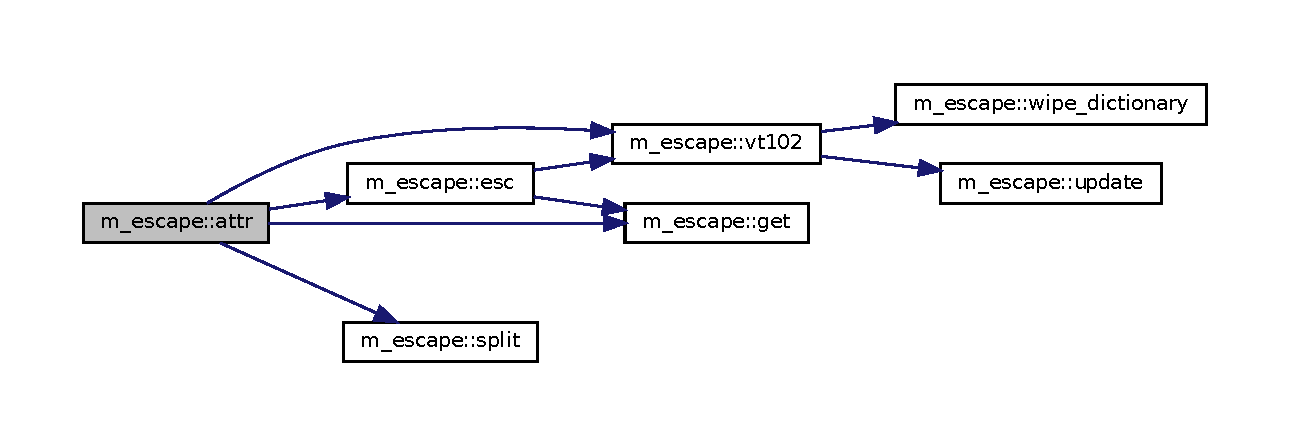
\includegraphics[width=350pt]{namespacem__escape_a916b16ce9be553d669f54cb9575a91be_cgraph}
\end{center}
\end{figure}
\mbox{\Hypertarget{namespacem__escape_af7d28a73e65efb58beeb684d7bdeefec}\label{namespacem__escape_af7d28a73e65efb58beeb684d7bdeefec}} 
\index{m\+\_\+escape@{m\+\_\+escape}!color@{color}}
\index{color@{color}!m\+\_\+escape@{m\+\_\+escape}}
\subsubsection{\texorpdfstring{color()}{color()}}
{\footnotesize\ttfamily character(len=\+:) function, allocatable, public m\+\_\+escape\+::color (\begin{DoxyParamCaption}\item[{character(len=$\ast$), intent(in)}]{string,  }\item[{character(len=$\ast$), intent(in), optional}]{fg,  }\item[{character(len=$\ast$), intent(in), optional}]{bg,  }\item[{character(len=$\ast$), intent(in), optional}]{style }\end{DoxyParamCaption})}



\subsubsection*{N\+A\+ME}

color(3f) -\/ \mbox{[}M\+\_\+escape\mbox{]} colorize text using a simple function-\/based approach (L\+I\+C\+E\+N\+SE\+:PD) \subsubsection*{S\+Y\+N\+O\+P\+S\+IS}

use M\+\_\+escape, only \+: color, color\+\_\+mode, \&

! F\+O\+R\+E\+G\+R\+O\+U\+ND C\+O\+L\+O\+RS \& fg\+\_\+red, fg\+\_\+cyan, fg\+\_\+magenta, fg\+\_\+blue, \& \& fg\+\_\+green, fg\+\_\+yellow, fg\+\_\+white, fg\+\_\+ebony, \& \& fg\+\_\+default, \& ! B\+A\+C\+K\+G\+R\+O\+U\+ND C\+O\+L\+O\+RS \& bg\+\_\+red, bg\+\_\+cyan, bg\+\_\+magenta, bg\+\_\+blue, \& \& bg\+\_\+green, bg\+\_\+yellow, bg\+\_\+white, bg\+\_\+ebony, \& \& bg\+\_\+default, \& ! A\+T\+T\+R\+I\+B\+U\+T\+ES \& bold, italic, inverse, underline, \& \& unbold, unitalic, uninverse, ununderline, \& \& reset, \& ! D\+I\+S\+P\+L\+AY \& clear

function color(string,fg,bg,style) result (out)

character(len=$\ast$),intent(in) \+:\+: string character(len=$\ast$),intent(in),optional \+:\+: fg character(len=$\ast$),intent(in),optional \+:\+: bg character(len=$\ast$),intent(in),optional \+:\+: style

\subsubsection*{D\+E\+S\+C\+R\+I\+P\+T\+I\+ON}

The color constant strings can be used directly but unconditionally in an output statement. To allow the attributes to be ignored they can be called with the color(3f) routine, which the color\+\_\+mode(3f) procedure can be used to toggle on and off. Note that this routine does an implicit reset at the end of each use.

\subsubsection*{O\+P\+T\+I\+O\+NS}

string string to assign attributes to fg foreground color constant bg background color constant style style keyword or concatenated style keywords

\subsubsection*{E\+X\+A\+M\+P\+LE}

Sample program

program demo\+\_\+color use M\+\_\+escape, only \+: color, color\+\_\+mode, \& ! F\+O\+R\+E\+G\+R\+O\+U\+ND C\+O\+L\+O\+RS \& fg\+\_\+red, fg\+\_\+cyan, fg\+\_\+magenta, fg\+\_\+blue, \& \& fg\+\_\+green, fg\+\_\+yellow, fg\+\_\+white, fg\+\_\+ebony, \& \& fg\+\_\+default, \& ! B\+A\+C\+K\+G\+R\+O\+U\+ND C\+O\+L\+O\+RS \& bg\+\_\+red, bg\+\_\+cyan, bg\+\_\+magenta, bg\+\_\+blue, \& \& bg\+\_\+green, bg\+\_\+yellow, bg\+\_\+white, bg\+\_\+ebony, \& \& bg\+\_\+default, \& ! A\+T\+T\+R\+I\+B\+U\+T\+ES \& bold, italic, inverse, underline, \& \& unbold, unitalic, uninverse, ununderline, \& \& reset, \& ! D\+I\+S\+P\+L\+AY \& clear implicit none write($\ast$,\textquotesingle{}($\ast$(g0))\textquotesingle{})fg\+\_\+red,bg\+\_\+green,bold,\textquotesingle{} Hello! \textquotesingle{},reset

write($\ast$,\textquotesingle{}(a)\textquotesingle{})color(\textquotesingle{} Hello! \textquotesingle{},fg=fg\+\_\+white,bg=bg\+\_\+red,style=italic//bold) call color\+\_\+mode(.false.) write($\ast$,\textquotesingle{}(a)\textquotesingle{})color(\textquotesingle{} Hello! \textquotesingle{},fg=fg\+\_\+red,bg=bg\+\_\+red,style=italic//bold) end program demo\+\_\+color

\subsubsection*{A\+U\+T\+H\+OR}

John S. Urban, 2020 \subsubsection*{L\+I\+C\+E\+N\+SE}

Public Domain 

References g\+\_\+color, and reset.

\mbox{\Hypertarget{namespacem__escape_a24566737cb6aa1672180eaa21c8d4f66}\label{namespacem__escape_a24566737cb6aa1672180eaa21c8d4f66}} 
\index{m\+\_\+escape@{m\+\_\+escape}!color\+\_\+mode@{color\+\_\+mode}}
\index{color\+\_\+mode@{color\+\_\+mode}!m\+\_\+escape@{m\+\_\+escape}}
\subsubsection{\texorpdfstring{color\+\_\+mode()}{color\_mode()}}
{\footnotesize\ttfamily subroutine, public m\+\_\+escape\+::color\+\_\+mode (\begin{DoxyParamCaption}\item[{logical, intent(in)}]{switch }\end{DoxyParamCaption})}



\subsubsection*{N\+A\+ME}

color\+\_\+mode(3f) -\/ \mbox{[}M\+\_\+escape\mbox{]} toggle style effects of color(3f) on and off (L\+I\+C\+E\+N\+SE\+:PD) \subsubsection*{S\+Y\+N\+O\+P\+S\+IS}

subroutine color\+\_\+mode(switch)

logical,intent(in) \+:\+: switch

\subsubsection*{D\+E\+S\+C\+R\+I\+P\+T\+I\+ON}

The color constant strings can be used directly but unconditionally in an output statement. To allow the attributes to be ignored they can be called with the color(3f) routine, which the color\+\_\+mode(3f) procedure can be used to toggle on and off. Note that this routine does an implicit reset at the end of each use.

\subsubsection*{O\+P\+T\+I\+O\+NS}

switch turn attributes set by color(3f) on and off

\subsubsection*{E\+X\+A\+M\+P\+LE}

Sample program

program demo\+\_\+color\+\_\+mode use M\+\_\+escape, only \+: color, color\+\_\+mode, \& ! F\+O\+R\+E\+G\+R\+O\+U\+ND C\+O\+L\+O\+RS \& fg\+\_\+red, fg\+\_\+cyan, fg\+\_\+magenta, fg\+\_\+blue, \& \& fg\+\_\+green, fg\+\_\+yellow, fg\+\_\+white, fg\+\_\+ebony, \& \& fg\+\_\+default, \& ! B\+A\+C\+K\+G\+R\+O\+U\+ND C\+O\+L\+O\+RS \& bg\+\_\+red, bg\+\_\+cyan, bg\+\_\+magenta, bg\+\_\+blue, \& \& bg\+\_\+green, bg\+\_\+yellow, bg\+\_\+white, bg\+\_\+ebony, \& \& bg\+\_\+default, \& ! A\+T\+T\+R\+I\+B\+U\+T\+ES \& bold, italic, inverse, underline, \& \& unbold, unitalic, uninverse, ununderline, \& \& reset, \& ! D\+I\+S\+P\+L\+AY \& clear implicit none write($\ast$,\textquotesingle{}($\ast$(g0))\textquotesingle{})fg\+\_\+red,bg\+\_\+green,bold,\textquotesingle{} Hello! \textquotesingle{},reset

write($\ast$,\textquotesingle{}(a)\textquotesingle{})color(\textquotesingle{} Hello! \textquotesingle{},fg=fg\+\_\+white,bg=bg\+\_\+red,style=italic//bold) call color\+\_\+mode(.false.) write($\ast$,\textquotesingle{}(a)\textquotesingle{})color(\textquotesingle{} Hello! \textquotesingle{},fg=fg\+\_\+red,bg=bg\+\_\+red,style=italic//bold) end program demo\+\_\+color\+\_\+mode

\subsubsection*{A\+U\+T\+H\+OR}

John S. Urban, 2020 \subsubsection*{L\+I\+C\+E\+N\+SE}

Public Domain 

References g\+\_\+color.

\mbox{\Hypertarget{namespacem__escape_a36f016baad6b23f86189e6f3ee6db0cb}\label{namespacem__escape_a36f016baad6b23f86189e6f3ee6db0cb}} 
\index{m\+\_\+escape@{m\+\_\+escape}!esc@{esc}}
\index{esc@{esc}!m\+\_\+escape@{m\+\_\+escape}}
\subsubsection{\texorpdfstring{esc()}{esc()}}
{\footnotesize\ttfamily character(len=\+:) function, allocatable, public m\+\_\+escape\+::esc (\begin{DoxyParamCaption}\item[{character(len=$\ast$), intent(in)}]{string,  }\item[{logical, intent(in), optional}]{clear\+\_\+at\+\_\+end }\end{DoxyParamCaption})}



\subsubsection*{N\+A\+ME}

esc(3f) -\/ \mbox{[}M\+\_\+escape\mbox{]} substitute escape sequences for X\+M\+L-\/like syntax in strings 

\subsubsection*{S\+Y\+N\+O\+P\+S\+IS}

\begin{DoxyVerb} function esc(string,clear_at_end) result (expanded)

   character(len=*),intent(in) :: string
   logical,intent(in),optional :: clear_at_end
   character(len=:),allocatable :: expanded
\end{DoxyVerb}


\subsubsection*{D\+E\+S\+C\+R\+I\+P\+T\+I\+ON}

Use X\+M\+L-\/like syntax to add attributes to terminal output such as color.

A\+N\+SI escape sequences are not universally supported by all terminal emulators; and normally should be suppressed when not going to a tty device. This routine provides the basic structure to support such behaviors.

\subsubsection*{O\+P\+T\+I\+O\+NS}

string input string of form \begin{DoxyVerb}            "<attribute_name>string</attribute_name> ...".

           where the current attributes are color names,
           bold, italic, underline, ...
\end{DoxyVerb}


clear\+\_\+at\+\_\+end By default, a sequence to clear all text attributes is sent at the end of the returned text if an escape character appears in the output string. This can be turned off by setting this value to false. \subsubsection*{K\+E\+Y\+W\+O\+R\+DS}

current keywords

colors\+: r, red, R, R\+ED g, green, G, G\+R\+E\+EN b, blue, B, B\+L\+UE m, magenta, M, M\+A\+G\+E\+N\+TA c, cyan, C, C\+Y\+AN y, yellow, Y, Y\+E\+L\+L\+OW e, ebony, E, E\+B\+O\+NY w, white, W, W\+H\+I\+TE attributes\+: it, italic bo, bold un, underline other\+: clear esc, escape default gt lt

By default, if the color mnemonics (ie. the keywords) are uppercase they change the background color. If lowercase, the foreground color.

The \char`\"{}default\char`\"{} keyword is typically used explicitly when clear\+\_\+at\+\_\+end=.false.

Add, delete, and replace what strings are produced using U\+P\+D\+A\+T\+E(3f).

\subsubsection*{L\+I\+M\+I\+T\+A\+T\+I\+O\+NS}

o colors are not nestable, keywords are case-\/sensitive, o not all terminals obey the sequences. On Windows, it is best if you use Windows 10+ and/or the Linux mode; although it has worked with all Cyg\+Win and Min\+GW and Putty windows and mintty. o you should use \char`\"{}$<$gt$>$\char`\"{} and \char`\"{}$<$lt$>$\char`\"{} instead of \char`\"{}$>$\char`\"{} and \char`\"{}$<$\char`\"{} in a string processed by esc(3f) instead of in any plain text output so that the raw mode will create correct input for the esc(3f) function if read back in.

\subsubsection*{E\+X\+A\+M\+P\+LE}

Sample program

program demo\+\_\+esc use M\+\_\+escape, only \+: esc, esc\+\_\+mode, update write($\ast$,\textquotesingle{}(a)\textquotesingle{}) esc(\textquotesingle{}$<$clear$>$T\+E\+ST D\+E\+F\+A\+U\+L\+TS\+:\textquotesingle{}) call printstuff()

write($\ast$,\textquotesingle{}(a)\textquotesingle{}) esc(\textquotesingle{}T\+E\+ST M\+A\+N\+N\+ER=P\+L\+A\+IN\+:\textquotesingle{}) call esc\+\_\+mode(manner=\textquotesingle{}plain\textquotesingle{}) call printstuff()

write($\ast$,\textquotesingle{}(a)\textquotesingle{}) esc(\textquotesingle{}T\+E\+ST M\+A\+N\+N\+ER=R\+AW\+:\textquotesingle{}) call esc\+\_\+mode(manner=\textquotesingle{}raw\textquotesingle{}) call printstuff()

write($\ast$,\textquotesingle{}(a)\textquotesingle{}) esc(\textquotesingle{}T\+E\+ST M\+A\+N\+N\+ER=color\+:\textquotesingle{}) call esc\+\_\+mode(manner=\textquotesingle{}color\textquotesingle{}) call printstuff()

write($\ast$,\textquotesingle{}(a)\textquotesingle{}) esc(\textquotesingle{}T\+E\+ST A\+D\+D\+I\+NG A C\+U\+S\+T\+OM S\+E\+Q\+U\+E\+N\+CE\+:\textquotesingle{}) call update(\textquotesingle{}blink\textquotesingle{},char(27)//\textquotesingle{}\mbox{[}5m\textquotesingle{}) call update(\textquotesingle{}/blink\textquotesingle{},char(27)//\textquotesingle{}\mbox{[}38m\textquotesingle{}) write($\ast$,\textquotesingle{}(a)\textquotesingle{}) esc(\textquotesingle{}$<$blink$>$Items for Friday$<$/blink$>$\textquotesingle{})

contains subroutine printstuff()

write($\ast$,\textquotesingle{}(a)\textquotesingle{}) esc(\textquotesingle{}$<$r$>$R\+ED$<$/r$>$,$<$g$>$G\+R\+E\+EN$<$/g$>$,{\bfseries B\+L\+UE}\textquotesingle{}) write($\ast$,\textquotesingle{}(a)\textquotesingle{}) esc(\textquotesingle{}{\ttfamily C\+Y\+AN},$<$m$>$M\+A\+G\+E\+N\+TA$<$/g$>$,$<$y$>$Y\+E\+L\+L\+OW$<$/y$>$\textquotesingle{}) write($\ast$,\textquotesingle{}(a)\textquotesingle{}) esc(\textquotesingle{}$<$w$>$W\+H\+I\+TE$<$/w$>$ and $<$e$>$E\+B\+O\+NY$<$/e$>$\textquotesingle{})

write($\ast$,\textquotesingle{}(a)\textquotesingle{}) esc(\textquotesingle{}Adding $<$bo$>$bold$<$/bo$>$\textquotesingle{}) write($\ast$,\textquotesingle{}(a)\textquotesingle{}) esc(\textquotesingle{}$<$bo$>$$<$r$>$R\+ED$<$/r$>$,$<$g$>$G\+R\+E\+EN$<$/g$>$,{\bfseries B\+L\+UE}$<$/bo$>$\textquotesingle{}) write($\ast$,\textquotesingle{}(a)\textquotesingle{}) esc(\textquotesingle{}$<$bo$>${\ttfamily C\+Y\+AN},$<$m$>$M\+A\+G\+E\+N\+TA$<$/g$>$,$<$y$>$Y\+E\+L\+L\+OW$<$/y$>$$<$/bo$>$\textquotesingle{}) write($\ast$,\textquotesingle{}(a)\textquotesingle{}) esc(\textquotesingle{}$<$bo$>$$<$w$>$W\+H\+I\+TE$<$/w$>$ and $<$e$>$E\+B\+O\+NY$<$/e$>$$<$/bo$>$\textquotesingle{})

write($\ast$,\textquotesingle{}(a)\textquotesingle{}) esc(\textquotesingle{}Adding 
\begin{DoxyItemize}
\item 
\end{DoxyItemize}\textquotesingle{}) write($\ast$,\textquotesingle{}(a)\textquotesingle{}) esc(\textquotesingle{}$<$bo$>$
\begin{DoxyItemize}
\item 
\end{DoxyItemize}$<$r$>$R\+ED$<$/r$>$,$<$g$>$G\+R\+E\+EN$<$/g$>$,{\bfseries B\+L\+UE}$<$/bo$>$\textquotesingle{}) write($\ast$,\textquotesingle{}(a)\textquotesingle{}) esc(\textquotesingle{}$<$bo$>$
\begin{DoxyItemize}
\item 
\end{DoxyItemize}{\ttfamily C\+Y\+AN},$<$m$>$M\+A\+G\+E\+N\+TA$<$/g$>$,$<$y$>$Y\+E\+L\+L\+OW$<$/y$>$$<$/bo$>$\textquotesingle{}) write($\ast$,\textquotesingle{}(a)\textquotesingle{}) esc(\textquotesingle{}$<$bo$>$
\begin{DoxyItemize}
\item 
\end{DoxyItemize}$<$w$>$W\+H\+I\+TE$<$/w$>$ and $<$e$>$E\+B\+O\+NY$<$/e$>$$<$/bo$>$\textquotesingle{})

write($\ast$,\textquotesingle{}(a)\textquotesingle{}) esc(\textquotesingle{}Adding 
\begin{DoxyItemize}
\item 
\end{DoxyItemize}\textquotesingle{}) write($\ast$,\textquotesingle{}(a)\textquotesingle{}) esc(\textquotesingle{}$<$bo$>$
\begin{DoxyItemize}
\item 
\end{DoxyItemize}$<$it$>$$<$r$>$R\+ED$<$/r$>$,$<$g$>$G\+R\+E\+EN$<$/g$>$,{\bfseries B\+L\+UE}$<$/it$>$$<$/bo$>$\textquotesingle{}) write($\ast$,\textquotesingle{}(a)\textquotesingle{}) esc(\textquotesingle{}$<$bo$>$
\begin{DoxyItemize}
\item 
\end{DoxyItemize}$<$it$>${\ttfamily C\+Y\+AN},$<$m$>$M\+A\+G\+E\+N\+TA$<$/g$>$,$<$y$>$Y\+E\+L\+L\+OW$<$/it$>$$<$/y$>$$<$/bo$>$\textquotesingle{}) write($\ast$,\textquotesingle{}(a)\textquotesingle{}) esc(\textquotesingle{}$<$bo$>$
\begin{DoxyItemize}
\item 
\end{DoxyItemize}$<$it$>$$<$w$>$W\+H\+I\+TE$<$/w$>$ and $<$e$>$E\+B\+O\+NY$<$/e$>$$<$/bo$>$\textquotesingle{})

write($\ast$,\textquotesingle{}(a)\textquotesingle{}) esc(\textquotesingle{}Adding $<$in$>$inverse$<$/in$>$\textquotesingle{}) write($\ast$,\textquotesingle{}(a)\textquotesingle{}) esc(\textquotesingle{}$<$in$>$$<$bo$>$
\begin{DoxyItemize}
\item 
\end{DoxyItemize}$<$it$>$$<$r$>$R\+ED$<$/r$>$,$<$g$>$G\+R\+E\+EN$<$/g$>$,{\bfseries B\+L\+UE}$<$/it$>$$<$/bo$>$$<$/in$>$\textquotesingle{}) write($\ast$,\textquotesingle{}(a)\textquotesingle{}) esc(\textquotesingle{}$<$in$>$$<$bo$>$
\begin{DoxyItemize}
\item 
\end{DoxyItemize}$<$it$>${\ttfamily C\+Y\+AN},$<$m$>$M\+A\+G\+E\+N\+TA$<$/g$>$,$<$y$>$Y\+E\+L\+L\+OW$<$/it$>$$<$/y$>$$<$/bo$>$$<$/in$>$\textquotesingle{}) write($\ast$,\textquotesingle{}(a)\textquotesingle{}) esc(\textquotesingle{}$<$in$>$$<$bo$>$
\begin{DoxyItemize}
\item 
\end{DoxyItemize}$<$it$>$$<$w$>$W\+H\+I\+TE$<$/w$>$ and $<$e$>$E\+B\+O\+NY$<$/e$>$$<$/bo$>$$<$/in$>$\textquotesingle{}) end subroutine printstuff

end program demo\+\_\+esc 

References code\+\_\+reset, debug, escape, get(), keywords, mode, and vt102().

Here is the call graph for this function\+:\nopagebreak
\begin{figure}[H]
\begin{center}
\leavevmode
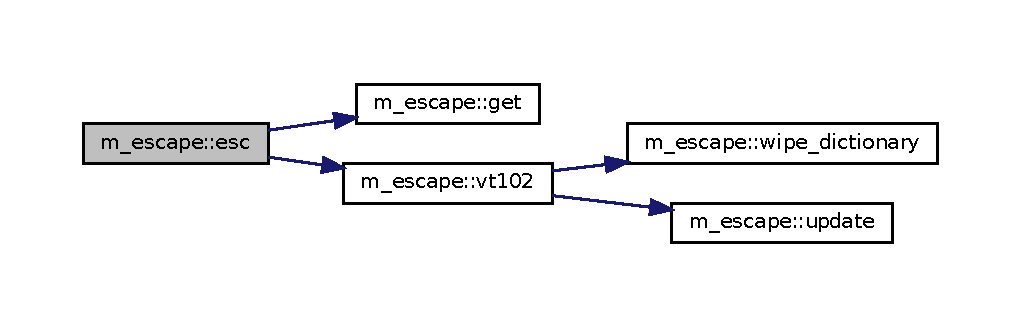
\includegraphics[width=350pt]{namespacem__escape_a36f016baad6b23f86189e6f3ee6db0cb_cgraph}
\end{center}
\end{figure}
Here is the caller graph for this function\+:\nopagebreak
\begin{figure}[H]
\begin{center}
\leavevmode
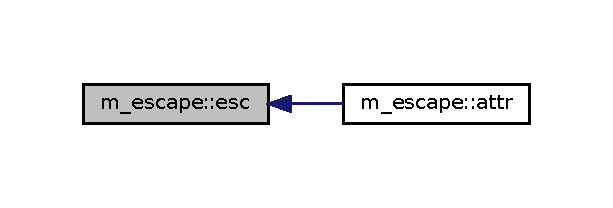
\includegraphics[width=294pt]{namespacem__escape_a36f016baad6b23f86189e6f3ee6db0cb_icgraph}
\end{center}
\end{figure}
\mbox{\Hypertarget{namespacem__escape_a4210456d81d9a1bf328093a9635e640b}\label{namespacem__escape_a4210456d81d9a1bf328093a9635e640b}} 
\index{m\+\_\+escape@{m\+\_\+escape}!esc\+\_\+mode@{esc\+\_\+mode}}
\index{esc\+\_\+mode@{esc\+\_\+mode}!m\+\_\+escape@{m\+\_\+escape}}
\subsubsection{\texorpdfstring{esc\+\_\+mode()}{esc\_mode()}}
{\footnotesize\ttfamily subroutine, public m\+\_\+escape\+::esc\+\_\+mode (\begin{DoxyParamCaption}\item[{character(len=$\ast$), intent(in)}]{manner }\end{DoxyParamCaption})}



\subsubsection*{N\+A\+ME}

esc\+\_\+mode(3f) -\/ \mbox{[}M\+\_\+escape\mbox{]} select processing mode for output from esc(3f) \subsubsection*{S\+Y\+N\+O\+P\+S\+IS}

subroutine esc\+\_\+mode(manner)

character(len=$\ast$),intent(in) \+:\+: manner \subsubsection*{D\+E\+S\+C\+R\+I\+P\+T\+I\+ON}

Turn off the generation of strings associated with the X\+ML keywords in the string generated by the esc(3f) function, or display the text in raw mode as it was passed to esc(3f) or return to A\+N\+SI escape control sequence generation.

\subsubsection*{O\+P\+T\+I\+O\+NS}

M\+A\+N\+N\+ER The current manners or modes supported via the E\+S\+C\+\_\+\+M\+O\+D\+E(3f) procedure are

plain suppress the output associated with keywords color(default) commonly supported escape sequences raw echo the input to E\+S\+C(3f) as its output reload restore original keyword meanings deleted or replaced by calls to update(3f).

\subsubsection*{E\+X\+A\+M\+P\+LE}

Sample program

program demo\+\_\+esc\+\_\+mode use M\+\_\+escape, only \+: esc, esc\+\_\+mode implicit none character(len=1024) \+:\+: line real \+:\+: value

value=3.\+4567 if( (value$>$0.\+0) .and. (value$<$100.\+0))then write(line,fmt=\textquotesingle{}(\char`\"{}\&
       \&$<$w$>$$<$\+G$>$\+G\+R\+E\+A\+T$<$/\+G$>$$<$/w$>$\+: The value $<$\+Y$>$$<$b$>$\char`\"{},f8.\+4,\char`\"{}$<$/b$>$$<$/\+Y$>$ is in range \&
       \&\char`\"{})\textquotesingle{})value else write(line,fmt=\textquotesingle{}(\char`\"{}\&
       \&$<$\+R$>$$<$e$>$\+E\+R\+R\+O\+R$<$/e$>$$<$/\+R$>$\+:\+The new value $<$\+Y$>$$<$b$>$\char`\"{},g0,\char`\"{}$<$/b$>$$<$/\+Y$>$ is out of range\&
       \& \char`\"{})\textquotesingle{})value endif

write($\ast$,\textquotesingle{}(a)\textquotesingle{})esc(trim(line))

call esc\+\_\+mode(manner=\textquotesingle{}plain\textquotesingle{}) ! write as plain text write($\ast$,\textquotesingle{}(a)\textquotesingle{})esc(trim(line)) call esc\+\_\+mode(manner=\textquotesingle{}raw\textquotesingle{}) ! write as-\/is write($\ast$,\textquotesingle{}(a)\textquotesingle{})esc(trim(line)) call esc\+\_\+mode(manner=\textquotesingle{}ansi\textquotesingle{}) ! return to default mode write($\ast$,\textquotesingle{}(a)\textquotesingle{})esc(trim(line))

end program demo\+\_\+esc\+\_\+mode 

References mode, and vt102().

Here is the call graph for this function\+:\nopagebreak
\begin{figure}[H]
\begin{center}
\leavevmode
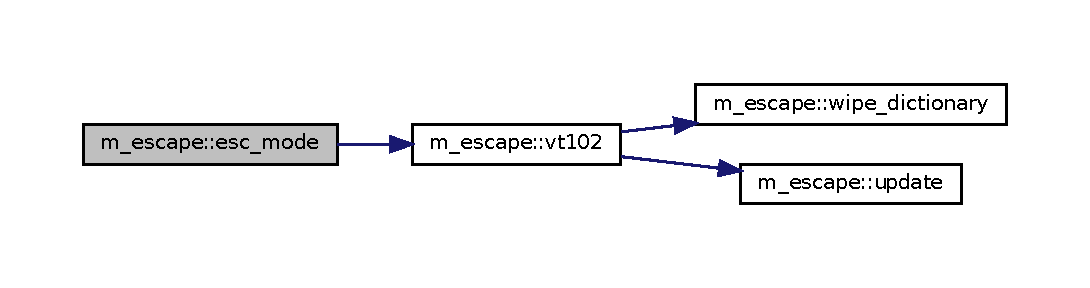
\includegraphics[width=350pt]{namespacem__escape_a4210456d81d9a1bf328093a9635e640b_cgraph}
\end{center}
\end{figure}
\mbox{\Hypertarget{namespacem__escape_af555c90c278ff964d8bce93ee0368a42}\label{namespacem__escape_af555c90c278ff964d8bce93ee0368a42}} 
\index{m\+\_\+escape@{m\+\_\+escape}!get@{get}}
\index{get@{get}!m\+\_\+escape@{m\+\_\+escape}}
\subsubsection{\texorpdfstring{get()}{get()}}
{\footnotesize\ttfamily character(len=\+:) function, allocatable m\+\_\+escape\+::get (\begin{DoxyParamCaption}\item[{character(len=$\ast$), intent(in)}]{key }\end{DoxyParamCaption})\hspace{0.3cm}{\ttfamily [private]}}



References counts, keywords, and values.

Here is the caller graph for this function\+:\nopagebreak
\begin{figure}[H]
\begin{center}
\leavevmode
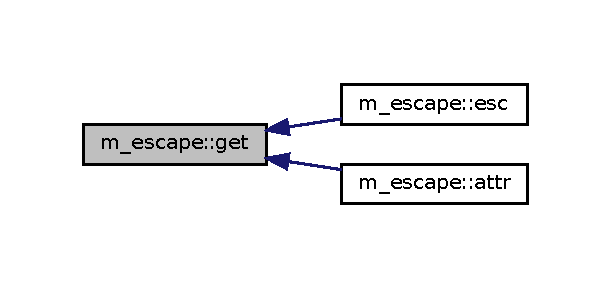
\includegraphics[width=350pt]{namespacem__escape_af555c90c278ff964d8bce93ee0368a42_icgraph}
\end{center}
\end{figure}
\mbox{\Hypertarget{namespacem__escape_a6add907828fd34e94b87f643a5cabc64}\label{namespacem__escape_a6add907828fd34e94b87f643a5cabc64}} 
\index{m\+\_\+escape@{m\+\_\+escape}!print\+\_\+dictionary@{print\+\_\+dictionary}}
\index{print\+\_\+dictionary@{print\+\_\+dictionary}!m\+\_\+escape@{m\+\_\+escape}}
\subsubsection{\texorpdfstring{print\+\_\+dictionary()}{print\_dictionary()}}
{\footnotesize\ttfamily subroutine, public m\+\_\+escape\+::print\+\_\+dictionary (\begin{DoxyParamCaption}\item[{character(len=$\ast$), intent(in), optional}]{header }\end{DoxyParamCaption})}



\subsubsection*{N\+A\+ME}

print\+\_\+dictionary(3f) -\/ \mbox{[}A\+R\+G\+U\+M\+E\+N\+TS\+:M\+\_\+\+C\+L\+I2\mbox{]} print internal dictionary created by calls to update(3f) (L\+I\+C\+E\+N\+SE\+:PD) \subsubsection*{S\+Y\+N\+O\+P\+S\+IS}

subroutine print\+\_\+dictionary(header)

character(len=$\ast$),intent(in),optional \+:\+: header \subsubsection*{D\+E\+S\+C\+R\+I\+P\+T\+I\+ON}

Print the internal dictionary created by calls to update(3f). This routine is intended to print the state of the argument list if an error occurs in using the update(3f) procedure. \subsubsection*{O\+P\+T\+I\+O\+NS}

H\+E\+A\+D\+ER label to print before printing the state of the command argument list. \subsubsection*{E\+X\+A\+M\+P\+LE}

Typical usage\+:

program demo\+\_\+print\+\_\+dictionary use M\+\_\+escape, only \+: esc, update, print\+\_\+dictionary implicit none write($\ast$,\textquotesingle{}(a)\textquotesingle{}) esc(\textquotesingle{}$<$clear$>$T\+E\+ST C\+U\+S\+T\+O\+M\+I\+Z\+ED\+:\textquotesingle{}) ! add custom keywords call update(\textquotesingle{}blink\textquotesingle{},char(27)//\textquotesingle{}\mbox{[}5m\textquotesingle{}) call update(\textquotesingle{}/blink\textquotesingle{},char(27)//\textquotesingle{}\mbox{[}38m\textquotesingle{}) call print\+\_\+dictionary(\textquotesingle{}D\+I\+C\+T\+I\+O\+N\+A\+RY\textquotesingle{}) write($\ast$,\textquotesingle{}(a)\textquotesingle{}) esc(\textquotesingle{}$<$blink$>$Items for Friday$<$/blink$>$\textquotesingle{}) end program demo\+\_\+print\+\_\+dictionary

Sample output

demo\+\_\+print\+\_\+dictionary $\vert$cat -\/v -\/e -\/t

\subsubsection*{A\+U\+T\+H\+OR}

John S. Urban, 2020 \subsubsection*{L\+I\+C\+E\+N\+SE}

Public Domain 

References counts, keywords, and values.

\mbox{\Hypertarget{namespacem__escape_af23bd97702864e0f32258e6ec0d51506}\label{namespacem__escape_af23bd97702864e0f32258e6ec0d51506}} 
\index{m\+\_\+escape@{m\+\_\+escape}!split@{split}}
\index{split@{split}!m\+\_\+escape@{m\+\_\+escape}}
\subsubsection{\texorpdfstring{split()}{split()}}
{\footnotesize\ttfamily subroutine m\+\_\+escape\+::split (\begin{DoxyParamCaption}\item[{character(len=$\ast$), intent(in)}]{input\+\_\+line,  }\item[{character(len=\+:), dimension(\+:), intent(out), allocatable}]{array,  }\item[{character(len=$\ast$), intent(in), optional}]{delimiters }\end{DoxyParamCaption})\hspace{0.3cm}{\ttfamily [private]}}

Here is the caller graph for this function\+:\nopagebreak
\begin{figure}[H]
\begin{center}
\leavevmode
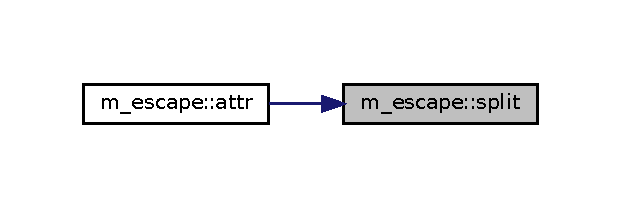
\includegraphics[width=298pt]{namespacem__escape_af23bd97702864e0f32258e6ec0d51506_icgraph}
\end{center}
\end{figure}
\mbox{\Hypertarget{namespacem__escape_a5efd612f60d281003917329484a7960c}\label{namespacem__escape_a5efd612f60d281003917329484a7960c}} 
\index{m\+\_\+escape@{m\+\_\+escape}!update@{update}}
\index{update@{update}!m\+\_\+escape@{m\+\_\+escape}}
\subsubsection{\texorpdfstring{update()}{update()}}
{\footnotesize\ttfamily subroutine, public m\+\_\+escape\+::update (\begin{DoxyParamCaption}\item[{character(len=$\ast$), intent(in)}]{key,  }\item[{character(len=$\ast$), intent(in), optional}]{valin }\end{DoxyParamCaption})}



\subsubsection*{N\+A\+ME}

update(3f) -\/ \mbox{[}M\+\_\+escape\mbox{]} update internal dictionary given keyword and value (L\+I\+C\+E\+N\+SE\+:PD) \subsubsection*{S\+Y\+N\+O\+P\+S\+IS}

subroutine update(key,val)

character(len=$\ast$),intent(in) \+:\+: key character(len=$\ast$),intent(in),optional \+:\+: val \subsubsection*{D\+E\+S\+C\+R\+I\+P\+T\+I\+ON}

Update internal dictionary in M\+\_\+escape(3fm) module. \subsubsection*{O\+P\+T\+I\+O\+NS}

key name of keyword to add, replace, or delete from dictionary val if present add or replace value associated with keyword. If not present remove keyword entry from dictionary. \subsubsection*{E\+X\+A\+M\+P\+LE}

Sample program

program demo\+\_\+update use M\+\_\+escape, only \+: esc, update write($\ast$,\textquotesingle{}(a)\textquotesingle{}) esc(\textquotesingle{}$<$clear$>$T\+E\+ST C\+U\+S\+T\+O\+M\+I\+Z\+ED\+:\textquotesingle{}) ! add custom keywords call update(\textquotesingle{}blink\textquotesingle{},char(27)//\textquotesingle{}\mbox{[}5m\textquotesingle{}) call update(\textquotesingle{}/blink\textquotesingle{},char(27)//\textquotesingle{}\mbox{[}38m\textquotesingle{})

write($\ast$,\textquotesingle{}(a)\textquotesingle{}) esc(\textquotesingle{}$<$blink$>$Items for Friday$<$/blink$>$\textquotesingle{})

write($\ast$,\textquotesingle{}(a)\textquotesingle{},advance=\textquotesingle{}no\textquotesingle{}) esc(\textquotesingle{}$<$r$>$R\+ED$<$/r$>$,\textquotesingle{}) write($\ast$,\textquotesingle{}(a)\textquotesingle{},advance=\textquotesingle{}no\textquotesingle{}) esc(\textquotesingle{}{\bfseries B\+L\+UE},\textquotesingle{}) write($\ast$,\textquotesingle{}(a)\textquotesingle{},advance=\textquotesingle{}yes\textquotesingle{}) esc(\textquotesingle{}$<$g$>$G\+R\+E\+EN$<$/g$>$\textquotesingle{})

! delete call update(\textquotesingle{}r\textquotesingle{}) call update(\textquotesingle{}/r\textquotesingle{}) ! replace call update(\textquotesingle{}b\textquotesingle{},\textquotesingle{}$<$$<$$<$$<$\textquotesingle{}) call update(\textquotesingle{}/b\textquotesingle{},\textquotesingle{}$>$$>$$>$$>$\textquotesingle{}) write($\ast$,\textquotesingle{}(a)\textquotesingle{},advance=\textquotesingle{}no\textquotesingle{}) esc(\textquotesingle{}$<$r$>$R\+ED$<$/r$>$,\textquotesingle{}) write($\ast$,\textquotesingle{}(a)\textquotesingle{},advance=\textquotesingle{}no\textquotesingle{}) esc(\textquotesingle{}{\bfseries B\+L\+UE},\textquotesingle{}) write($\ast$,\textquotesingle{}(a)\textquotesingle{},advance=\textquotesingle{}yes\textquotesingle{}) esc(\textquotesingle{}$<$g$>$G\+R\+E\+EN$<$/g$>$\textquotesingle{})

end program demo\+\_\+update

\subsubsection*{A\+U\+T\+H\+OR}

John S. Urban, 2020 \subsubsection*{L\+I\+C\+E\+N\+SE}

Public Domain 

References counts, keywords, and values.

Here is the caller graph for this function\+:\nopagebreak
\begin{figure}[H]
\begin{center}
\leavevmode
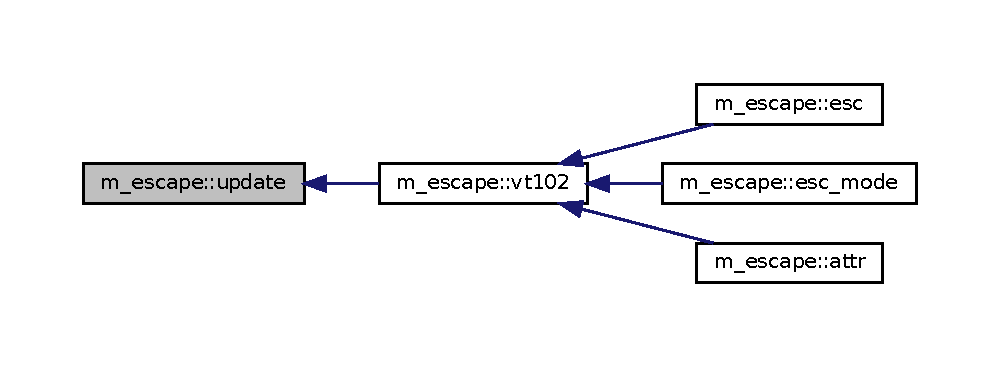
\includegraphics[width=350pt]{namespacem__escape_a5efd612f60d281003917329484a7960c_icgraph}
\end{center}
\end{figure}
\mbox{\Hypertarget{namespacem__escape_ae9d40717b2e75e90e2505d5fed6435c5}\label{namespacem__escape_ae9d40717b2e75e90e2505d5fed6435c5}} 
\index{m\+\_\+escape@{m\+\_\+escape}!vt102@{vt102}}
\index{vt102@{vt102}!m\+\_\+escape@{m\+\_\+escape}}
\subsubsection{\texorpdfstring{vt102()}{vt102()}}
{\footnotesize\ttfamily subroutine m\+\_\+escape\+::vt102 (\begin{DoxyParamCaption}{ }\end{DoxyParamCaption})\hspace{0.3cm}{\ttfamily [private]}}



References bell, bg\+\_\+blue, bg\+\_\+cyan, bg\+\_\+default, bg\+\_\+ebony, bg\+\_\+green, bg\+\_\+magenta, bg\+\_\+red, bg\+\_\+white, bg\+\_\+yellow, bold, clear, escape, fg\+\_\+blue, fg\+\_\+cyan, fg\+\_\+default, fg\+\_\+ebony, fg\+\_\+green, fg\+\_\+magenta, fg\+\_\+red, fg\+\_\+white, fg\+\_\+yellow, inverse, italic, reset, unbold, underline, uninverse, unitalic, ununderline, update(), and wipe\+\_\+dictionary().

Here is the call graph for this function\+:\nopagebreak
\begin{figure}[H]
\begin{center}
\leavevmode
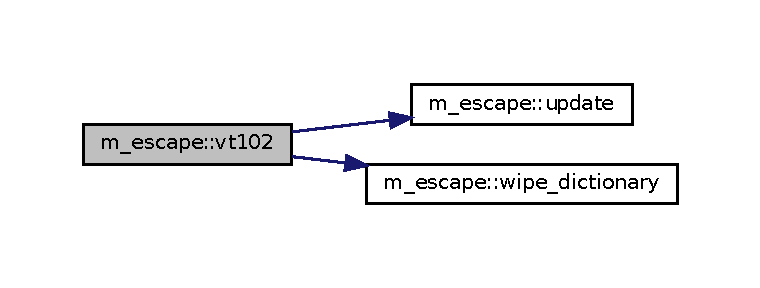
\includegraphics[width=350pt]{namespacem__escape_ae9d40717b2e75e90e2505d5fed6435c5_cgraph}
\end{center}
\end{figure}
Here is the caller graph for this function\+:\nopagebreak
\begin{figure}[H]
\begin{center}
\leavevmode
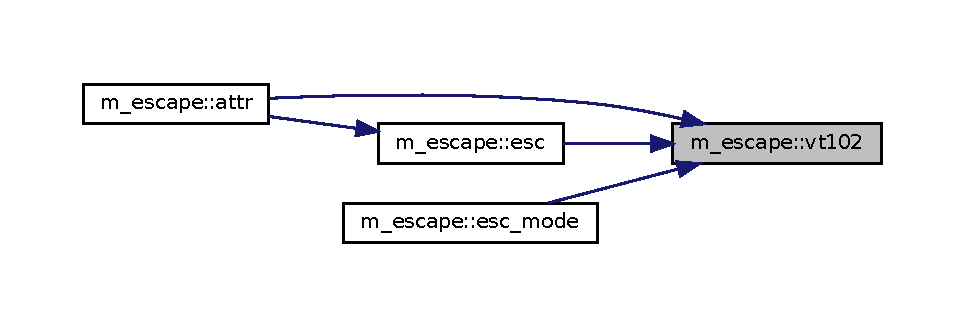
\includegraphics[width=350pt]{namespacem__escape_ae9d40717b2e75e90e2505d5fed6435c5_icgraph}
\end{center}
\end{figure}
\mbox{\Hypertarget{namespacem__escape_a1bc574bc97157fe67d868d2bd180c91e}\label{namespacem__escape_a1bc574bc97157fe67d868d2bd180c91e}} 
\index{m\+\_\+escape@{m\+\_\+escape}!wipe\+\_\+dictionary@{wipe\+\_\+dictionary}}
\index{wipe\+\_\+dictionary@{wipe\+\_\+dictionary}!m\+\_\+escape@{m\+\_\+escape}}
\subsubsection{\texorpdfstring{wipe\+\_\+dictionary()}{wipe\_dictionary()}}
{\footnotesize\ttfamily subroutine m\+\_\+escape\+::wipe\+\_\+dictionary (\begin{DoxyParamCaption}{ }\end{DoxyParamCaption})\hspace{0.3cm}{\ttfamily [private]}}



References counts, keywords, and values.

Here is the caller graph for this function\+:\nopagebreak
\begin{figure}[H]
\begin{center}
\leavevmode
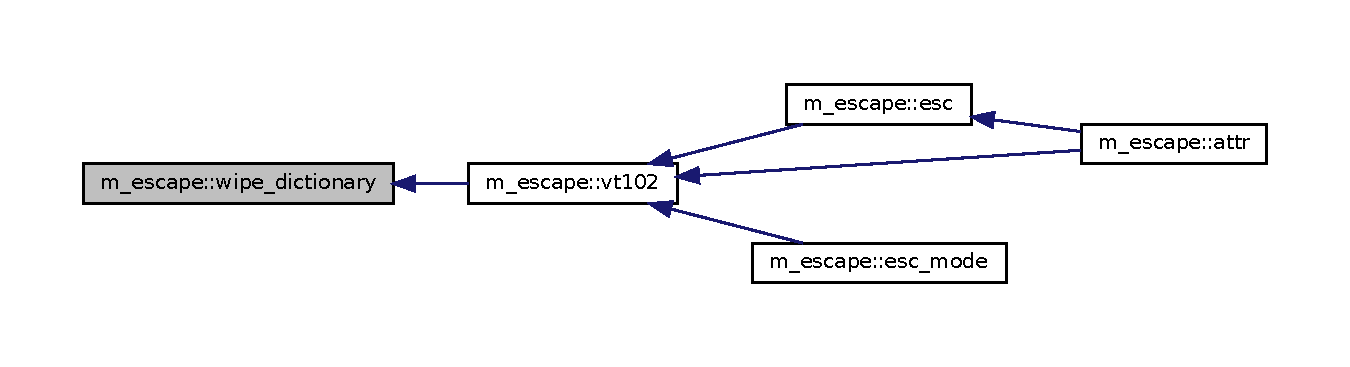
\includegraphics[width=350pt]{namespacem__escape_a1bc574bc97157fe67d868d2bd180c91e_icgraph}
\end{center}
\end{figure}


\subsection{Variable Documentation}
\mbox{\Hypertarget{namespacem__escape_a2cd9c30d3783af9d1f74a50e7f1dbd7f}\label{namespacem__escape_a2cd9c30d3783af9d1f74a50e7f1dbd7f}} 
\index{m\+\_\+escape@{m\+\_\+escape}!bell@{bell}}
\index{bell@{bell}!m\+\_\+escape@{m\+\_\+escape}}
\subsubsection{\texorpdfstring{bell}{bell}}
{\footnotesize\ttfamily character(len=$\ast$), parameter m\+\_\+escape\+::bell =achar(7)\hspace{0.3cm}{\ttfamily [private]}}

\mbox{\Hypertarget{namespacem__escape_a2f34e53ba01ebac10ab70f25e3c9727a}\label{namespacem__escape_a2f34e53ba01ebac10ab70f25e3c9727a}} 
\index{m\+\_\+escape@{m\+\_\+escape}!bg\+\_\+black@{bg\+\_\+black}}
\index{bg\+\_\+black@{bg\+\_\+black}!m\+\_\+escape@{m\+\_\+escape}}
\subsubsection{\texorpdfstring{bg\+\_\+black}{bg\_black}}
{\footnotesize\ttfamily character(len=$\ast$), parameter, public m\+\_\+escape\+::bg\+\_\+black = C\+O\+D\+E\+\_\+\+S\+T\+A\+RT//C\+O\+L\+O\+R\+\_\+\+B\+G\+\_\+\+B\+L\+A\+CK//C\+O\+D\+E\+\_\+\+E\+ND}

\mbox{\Hypertarget{namespacem__escape_afab2229302287eaa0eb05add07bb6621}\label{namespacem__escape_afab2229302287eaa0eb05add07bb6621}} 
\index{m\+\_\+escape@{m\+\_\+escape}!bg\+\_\+blue@{bg\+\_\+blue}}
\index{bg\+\_\+blue@{bg\+\_\+blue}!m\+\_\+escape@{m\+\_\+escape}}
\subsubsection{\texorpdfstring{bg\+\_\+blue}{bg\_blue}}
{\footnotesize\ttfamily character(len=$\ast$), parameter, public m\+\_\+escape\+::bg\+\_\+blue = C\+O\+D\+E\+\_\+\+S\+T\+A\+RT//C\+O\+L\+O\+R\+\_\+\+B\+G\+\_\+\+B\+L\+UE//C\+O\+D\+E\+\_\+\+E\+ND}

\mbox{\Hypertarget{namespacem__escape_a7b7a979cd6dc44533f962d323c65a7b6}\label{namespacem__escape_a7b7a979cd6dc44533f962d323c65a7b6}} 
\index{m\+\_\+escape@{m\+\_\+escape}!bg\+\_\+cyan@{bg\+\_\+cyan}}
\index{bg\+\_\+cyan@{bg\+\_\+cyan}!m\+\_\+escape@{m\+\_\+escape}}
\subsubsection{\texorpdfstring{bg\+\_\+cyan}{bg\_cyan}}
{\footnotesize\ttfamily character(len=$\ast$), parameter, public m\+\_\+escape\+::bg\+\_\+cyan = C\+O\+D\+E\+\_\+\+S\+T\+A\+RT//C\+O\+L\+O\+R\+\_\+\+B\+G\+\_\+\+C\+Y\+AN//C\+O\+D\+E\+\_\+\+E\+ND}

\mbox{\Hypertarget{namespacem__escape_a329b88dbfe4ad42f896cdf408dcd9784}\label{namespacem__escape_a329b88dbfe4ad42f896cdf408dcd9784}} 
\index{m\+\_\+escape@{m\+\_\+escape}!bg\+\_\+default@{bg\+\_\+default}}
\index{bg\+\_\+default@{bg\+\_\+default}!m\+\_\+escape@{m\+\_\+escape}}
\subsubsection{\texorpdfstring{bg\+\_\+default}{bg\_default}}
{\footnotesize\ttfamily character(len=$\ast$), parameter, public m\+\_\+escape\+::bg\+\_\+default = C\+O\+D\+E\+\_\+\+S\+T\+A\+RT//C\+O\+L\+O\+R\+\_\+\+B\+G\+\_\+\+D\+E\+F\+A\+U\+LT//C\+O\+D\+E\+\_\+\+E\+ND}

\mbox{\Hypertarget{namespacem__escape_ab3691cc02cfaf12d6f7e18fac8a70b0b}\label{namespacem__escape_ab3691cc02cfaf12d6f7e18fac8a70b0b}} 
\index{m\+\_\+escape@{m\+\_\+escape}!bg\+\_\+ebony@{bg\+\_\+ebony}}
\index{bg\+\_\+ebony@{bg\+\_\+ebony}!m\+\_\+escape@{m\+\_\+escape}}
\subsubsection{\texorpdfstring{bg\+\_\+ebony}{bg\_ebony}}
{\footnotesize\ttfamily character(len=$\ast$), parameter, public m\+\_\+escape\+::bg\+\_\+ebony = C\+O\+D\+E\+\_\+\+S\+T\+A\+RT//C\+O\+L\+O\+R\+\_\+\+B\+G\+\_\+\+B\+L\+A\+CK//C\+O\+D\+E\+\_\+\+E\+ND}

\mbox{\Hypertarget{namespacem__escape_a5754e4af92f738d3fd7c95daeaa7f2e1}\label{namespacem__escape_a5754e4af92f738d3fd7c95daeaa7f2e1}} 
\index{m\+\_\+escape@{m\+\_\+escape}!bg\+\_\+green@{bg\+\_\+green}}
\index{bg\+\_\+green@{bg\+\_\+green}!m\+\_\+escape@{m\+\_\+escape}}
\subsubsection{\texorpdfstring{bg\+\_\+green}{bg\_green}}
{\footnotesize\ttfamily character(len=$\ast$), parameter, public m\+\_\+escape\+::bg\+\_\+green = C\+O\+D\+E\+\_\+\+S\+T\+A\+RT//C\+O\+L\+O\+R\+\_\+\+B\+G\+\_\+\+G\+R\+E\+EN//C\+O\+D\+E\+\_\+\+E\+ND}

\mbox{\Hypertarget{namespacem__escape_aaf244507d267d0ae99ea933a8744c7e4}\label{namespacem__escape_aaf244507d267d0ae99ea933a8744c7e4}} 
\index{m\+\_\+escape@{m\+\_\+escape}!bg\+\_\+magenta@{bg\+\_\+magenta}}
\index{bg\+\_\+magenta@{bg\+\_\+magenta}!m\+\_\+escape@{m\+\_\+escape}}
\subsubsection{\texorpdfstring{bg\+\_\+magenta}{bg\_magenta}}
{\footnotesize\ttfamily character(len=$\ast$), parameter, public m\+\_\+escape\+::bg\+\_\+magenta = C\+O\+D\+E\+\_\+\+S\+T\+A\+RT//C\+O\+L\+O\+R\+\_\+\+B\+G\+\_\+\+M\+A\+G\+E\+N\+TA//C\+O\+D\+E\+\_\+\+E\+ND}

\mbox{\Hypertarget{namespacem__escape_a3cd9ef6cdd5ab3dda36cc9402dff0806}\label{namespacem__escape_a3cd9ef6cdd5ab3dda36cc9402dff0806}} 
\index{m\+\_\+escape@{m\+\_\+escape}!bg\+\_\+red@{bg\+\_\+red}}
\index{bg\+\_\+red@{bg\+\_\+red}!m\+\_\+escape@{m\+\_\+escape}}
\subsubsection{\texorpdfstring{bg\+\_\+red}{bg\_red}}
{\footnotesize\ttfamily character(len=$\ast$), parameter, public m\+\_\+escape\+::bg\+\_\+red = C\+O\+D\+E\+\_\+\+S\+T\+A\+RT//C\+O\+L\+O\+R\+\_\+\+B\+G\+\_\+\+R\+ED//C\+O\+D\+E\+\_\+\+E\+ND}

\mbox{\Hypertarget{namespacem__escape_a87dfd88e3190a8717cc574d4f2a4445c}\label{namespacem__escape_a87dfd88e3190a8717cc574d4f2a4445c}} 
\index{m\+\_\+escape@{m\+\_\+escape}!bg\+\_\+white@{bg\+\_\+white}}
\index{bg\+\_\+white@{bg\+\_\+white}!m\+\_\+escape@{m\+\_\+escape}}
\subsubsection{\texorpdfstring{bg\+\_\+white}{bg\_white}}
{\footnotesize\ttfamily character(len=$\ast$), parameter, public m\+\_\+escape\+::bg\+\_\+white = C\+O\+D\+E\+\_\+\+S\+T\+A\+RT//C\+O\+L\+O\+R\+\_\+\+B\+G\+\_\+\+W\+H\+I\+TE//C\+O\+D\+E\+\_\+\+E\+ND}

\mbox{\Hypertarget{namespacem__escape_afe23b71a7646ac88c8c74358994f92d0}\label{namespacem__escape_afe23b71a7646ac88c8c74358994f92d0}} 
\index{m\+\_\+escape@{m\+\_\+escape}!bg\+\_\+yellow@{bg\+\_\+yellow}}
\index{bg\+\_\+yellow@{bg\+\_\+yellow}!m\+\_\+escape@{m\+\_\+escape}}
\subsubsection{\texorpdfstring{bg\+\_\+yellow}{bg\_yellow}}
{\footnotesize\ttfamily character(len=$\ast$), parameter, public m\+\_\+escape\+::bg\+\_\+yellow = C\+O\+D\+E\+\_\+\+S\+T\+A\+RT//C\+O\+L\+O\+R\+\_\+\+B\+G\+\_\+\+Y\+E\+L\+L\+OW//C\+O\+D\+E\+\_\+\+E\+ND}

\mbox{\Hypertarget{namespacem__escape_a9a369de1d051ce7fdbdedcba4574c962}\label{namespacem__escape_a9a369de1d051ce7fdbdedcba4574c962}} 
\index{m\+\_\+escape@{m\+\_\+escape}!bold@{bold}}
\index{bold@{bold}!m\+\_\+escape@{m\+\_\+escape}}
\subsubsection{\texorpdfstring{bold}{bold}}
{\footnotesize\ttfamily character(len=$\ast$), parameter, public m\+\_\+escape\+::bold = C\+O\+D\+E\+\_\+\+S\+T\+A\+RT//B\+O\+L\+D\+\_\+\+ON//C\+O\+D\+E\+\_\+\+E\+ND}

\mbox{\Hypertarget{namespacem__escape_a978fe9a5d07621c57c3163d8a7a62118}\label{namespacem__escape_a978fe9a5d07621c57c3163d8a7a62118}} 
\index{m\+\_\+escape@{m\+\_\+escape}!bold\+\_\+off@{bold\+\_\+off}}
\index{bold\+\_\+off@{bold\+\_\+off}!m\+\_\+escape@{m\+\_\+escape}}
\subsubsection{\texorpdfstring{bold\+\_\+off}{bold\_off}}
{\footnotesize\ttfamily character(len=$\ast$), parameter m\+\_\+escape\+::bold\+\_\+off =\textquotesingle{}22\textquotesingle{}\hspace{0.3cm}{\ttfamily [private]}}

\mbox{\Hypertarget{namespacem__escape_a8f30470c66af08cf881d9afe23357a03}\label{namespacem__escape_a8f30470c66af08cf881d9afe23357a03}} 
\index{m\+\_\+escape@{m\+\_\+escape}!bold\+\_\+on@{bold\+\_\+on}}
\index{bold\+\_\+on@{bold\+\_\+on}!m\+\_\+escape@{m\+\_\+escape}}
\subsubsection{\texorpdfstring{bold\+\_\+on}{bold\_on}}
{\footnotesize\ttfamily character(len=$\ast$), parameter m\+\_\+escape\+::bold\+\_\+on =\textquotesingle{}1\textquotesingle{}\hspace{0.3cm}{\ttfamily [private]}}

\mbox{\Hypertarget{namespacem__escape_a49210f3a0332fb37df08c519b3252bef}\label{namespacem__escape_a49210f3a0332fb37df08c519b3252bef}} 
\index{m\+\_\+escape@{m\+\_\+escape}!clear@{clear}}
\index{clear@{clear}!m\+\_\+escape@{m\+\_\+escape}}
\subsubsection{\texorpdfstring{clear}{clear}}
{\footnotesize\ttfamily character(len=$\ast$), parameter, public m\+\_\+escape\+::clear = H\+O\+M\+E\+\_\+\+D\+I\+S\+P\+L\+AY//C\+L\+E\+A\+R\+\_\+\+D\+I\+S\+P\+L\+AY}

\mbox{\Hypertarget{namespacem__escape_a9d45e30ea5891b89dc9a61ba1b5dbc03}\label{namespacem__escape_a9d45e30ea5891b89dc9a61ba1b5dbc03}} 
\index{m\+\_\+escape@{m\+\_\+escape}!clear\+\_\+display@{clear\+\_\+display}}
\index{clear\+\_\+display@{clear\+\_\+display}!m\+\_\+escape@{m\+\_\+escape}}
\subsubsection{\texorpdfstring{clear\+\_\+display}{clear\_display}}
{\footnotesize\ttfamily character(len=$\ast$), parameter m\+\_\+escape\+::clear\+\_\+display =C\+O\+D\+E\+\_\+\+S\+T\+A\+RT//\textquotesingle{}2\+J\textquotesingle{}\hspace{0.3cm}{\ttfamily [private]}}

\mbox{\Hypertarget{namespacem__escape_af913c326395b9bf2c089c30698d2c742}\label{namespacem__escape_af913c326395b9bf2c089c30698d2c742}} 
\index{m\+\_\+escape@{m\+\_\+escape}!code\+\_\+end@{code\+\_\+end}}
\index{code\+\_\+end@{code\+\_\+end}!m\+\_\+escape@{m\+\_\+escape}}
\subsubsection{\texorpdfstring{code\+\_\+end}{code\_end}}
{\footnotesize\ttfamily character(len=$\ast$), parameter m\+\_\+escape\+::code\+\_\+end =\textquotesingle{}m\textquotesingle{}\hspace{0.3cm}{\ttfamily [private]}}

\mbox{\Hypertarget{namespacem__escape_aaaf7224f2104dcd571cdaa69b61b9d01}\label{namespacem__escape_aaaf7224f2104dcd571cdaa69b61b9d01}} 
\index{m\+\_\+escape@{m\+\_\+escape}!code\+\_\+reset@{code\+\_\+reset}}
\index{code\+\_\+reset@{code\+\_\+reset}!m\+\_\+escape@{m\+\_\+escape}}
\subsubsection{\texorpdfstring{code\+\_\+reset}{code\_reset}}
{\footnotesize\ttfamily character(len=$\ast$), parameter m\+\_\+escape\+::code\+\_\+reset =C\+O\+D\+E\+\_\+\+S\+T\+A\+RT//\textquotesingle{}0\textquotesingle{}//C\+O\+D\+E\+\_\+\+E\+ND\hspace{0.3cm}{\ttfamily [private]}}

\mbox{\Hypertarget{namespacem__escape_a6d5af6b1571cba22511523c53c71fa6f}\label{namespacem__escape_a6d5af6b1571cba22511523c53c71fa6f}} 
\index{m\+\_\+escape@{m\+\_\+escape}!code\+\_\+start@{code\+\_\+start}}
\index{code\+\_\+start@{code\+\_\+start}!m\+\_\+escape@{m\+\_\+escape}}
\subsubsection{\texorpdfstring{code\+\_\+start}{code\_start}}
{\footnotesize\ttfamily character(len=$\ast$), parameter m\+\_\+escape\+::code\+\_\+start =E\+S\+C\+A\+PE//\textquotesingle{}\mbox{[}\textquotesingle{}\hspace{0.3cm}{\ttfamily [private]}}

\mbox{\Hypertarget{namespacem__escape_a5e4fc9941494a5c9518c84b434bfc97b}\label{namespacem__escape_a5e4fc9941494a5c9518c84b434bfc97b}} 
\index{m\+\_\+escape@{m\+\_\+escape}!color\+\_\+bg\+\_\+black@{color\+\_\+bg\+\_\+black}}
\index{color\+\_\+bg\+\_\+black@{color\+\_\+bg\+\_\+black}!m\+\_\+escape@{m\+\_\+escape}}
\subsubsection{\texorpdfstring{color\+\_\+bg\+\_\+black}{color\_bg\_black}}
{\footnotesize\ttfamily character(len=$\ast$), parameter m\+\_\+escape\+::color\+\_\+bg\+\_\+black =\textquotesingle{}40\textquotesingle{}\hspace{0.3cm}{\ttfamily [private]}}

\mbox{\Hypertarget{namespacem__escape_a80a991f9ee93243b6b9bea07f2ec6d03}\label{namespacem__escape_a80a991f9ee93243b6b9bea07f2ec6d03}} 
\index{m\+\_\+escape@{m\+\_\+escape}!color\+\_\+bg\+\_\+black\+\_\+intense@{color\+\_\+bg\+\_\+black\+\_\+intense}}
\index{color\+\_\+bg\+\_\+black\+\_\+intense@{color\+\_\+bg\+\_\+black\+\_\+intense}!m\+\_\+escape@{m\+\_\+escape}}
\subsubsection{\texorpdfstring{color\+\_\+bg\+\_\+black\+\_\+intense}{color\_bg\_black\_intense}}
{\footnotesize\ttfamily character(len=$\ast$), parameter m\+\_\+escape\+::color\+\_\+bg\+\_\+black\+\_\+intense =\textquotesingle{}100\textquotesingle{}\hspace{0.3cm}{\ttfamily [private]}}

\mbox{\Hypertarget{namespacem__escape_a699e7848c3c43f328168d59211d054cc}\label{namespacem__escape_a699e7848c3c43f328168d59211d054cc}} 
\index{m\+\_\+escape@{m\+\_\+escape}!color\+\_\+bg\+\_\+blue@{color\+\_\+bg\+\_\+blue}}
\index{color\+\_\+bg\+\_\+blue@{color\+\_\+bg\+\_\+blue}!m\+\_\+escape@{m\+\_\+escape}}
\subsubsection{\texorpdfstring{color\+\_\+bg\+\_\+blue}{color\_bg\_blue}}
{\footnotesize\ttfamily character(len=$\ast$), parameter m\+\_\+escape\+::color\+\_\+bg\+\_\+blue =\textquotesingle{}44\textquotesingle{}\hspace{0.3cm}{\ttfamily [private]}}

\mbox{\Hypertarget{namespacem__escape_aac30abbb8eb6e1570e28dac2326113a7}\label{namespacem__escape_aac30abbb8eb6e1570e28dac2326113a7}} 
\index{m\+\_\+escape@{m\+\_\+escape}!color\+\_\+bg\+\_\+blue\+\_\+intense@{color\+\_\+bg\+\_\+blue\+\_\+intense}}
\index{color\+\_\+bg\+\_\+blue\+\_\+intense@{color\+\_\+bg\+\_\+blue\+\_\+intense}!m\+\_\+escape@{m\+\_\+escape}}
\subsubsection{\texorpdfstring{color\+\_\+bg\+\_\+blue\+\_\+intense}{color\_bg\_blue\_intense}}
{\footnotesize\ttfamily character(len=$\ast$), parameter m\+\_\+escape\+::color\+\_\+bg\+\_\+blue\+\_\+intense =\textquotesingle{}104\textquotesingle{}\hspace{0.3cm}{\ttfamily [private]}}

\mbox{\Hypertarget{namespacem__escape_a895ed90037352c2ce2be6353f6764cb8}\label{namespacem__escape_a895ed90037352c2ce2be6353f6764cb8}} 
\index{m\+\_\+escape@{m\+\_\+escape}!color\+\_\+bg\+\_\+cyan@{color\+\_\+bg\+\_\+cyan}}
\index{color\+\_\+bg\+\_\+cyan@{color\+\_\+bg\+\_\+cyan}!m\+\_\+escape@{m\+\_\+escape}}
\subsubsection{\texorpdfstring{color\+\_\+bg\+\_\+cyan}{color\_bg\_cyan}}
{\footnotesize\ttfamily character(len=$\ast$), parameter m\+\_\+escape\+::color\+\_\+bg\+\_\+cyan =\textquotesingle{}46\textquotesingle{}\hspace{0.3cm}{\ttfamily [private]}}

\mbox{\Hypertarget{namespacem__escape_a6be9fe26e904b8714e035412ae4e6ad4}\label{namespacem__escape_a6be9fe26e904b8714e035412ae4e6ad4}} 
\index{m\+\_\+escape@{m\+\_\+escape}!color\+\_\+bg\+\_\+cyan\+\_\+intense@{color\+\_\+bg\+\_\+cyan\+\_\+intense}}
\index{color\+\_\+bg\+\_\+cyan\+\_\+intense@{color\+\_\+bg\+\_\+cyan\+\_\+intense}!m\+\_\+escape@{m\+\_\+escape}}
\subsubsection{\texorpdfstring{color\+\_\+bg\+\_\+cyan\+\_\+intense}{color\_bg\_cyan\_intense}}
{\footnotesize\ttfamily character(len=$\ast$), parameter m\+\_\+escape\+::color\+\_\+bg\+\_\+cyan\+\_\+intense =\textquotesingle{}106\textquotesingle{}\hspace{0.3cm}{\ttfamily [private]}}

\mbox{\Hypertarget{namespacem__escape_af84f93410fbe9fa8fea3b02ac9371833}\label{namespacem__escape_af84f93410fbe9fa8fea3b02ac9371833}} 
\index{m\+\_\+escape@{m\+\_\+escape}!color\+\_\+bg\+\_\+default@{color\+\_\+bg\+\_\+default}}
\index{color\+\_\+bg\+\_\+default@{color\+\_\+bg\+\_\+default}!m\+\_\+escape@{m\+\_\+escape}}
\subsubsection{\texorpdfstring{color\+\_\+bg\+\_\+default}{color\_bg\_default}}
{\footnotesize\ttfamily character(len=$\ast$), parameter m\+\_\+escape\+::color\+\_\+bg\+\_\+default =\textquotesingle{}49\textquotesingle{}\hspace{0.3cm}{\ttfamily [private]}}

\mbox{\Hypertarget{namespacem__escape_a7c50b2b50909acf5935f9de7642d30f3}\label{namespacem__escape_a7c50b2b50909acf5935f9de7642d30f3}} 
\index{m\+\_\+escape@{m\+\_\+escape}!color\+\_\+bg\+\_\+green@{color\+\_\+bg\+\_\+green}}
\index{color\+\_\+bg\+\_\+green@{color\+\_\+bg\+\_\+green}!m\+\_\+escape@{m\+\_\+escape}}
\subsubsection{\texorpdfstring{color\+\_\+bg\+\_\+green}{color\_bg\_green}}
{\footnotesize\ttfamily character(len=$\ast$), parameter m\+\_\+escape\+::color\+\_\+bg\+\_\+green =\textquotesingle{}42\textquotesingle{}\hspace{0.3cm}{\ttfamily [private]}}

\mbox{\Hypertarget{namespacem__escape_a9ee5d5f2d0522ca3ea194de4d9a05dc3}\label{namespacem__escape_a9ee5d5f2d0522ca3ea194de4d9a05dc3}} 
\index{m\+\_\+escape@{m\+\_\+escape}!color\+\_\+bg\+\_\+green\+\_\+intense@{color\+\_\+bg\+\_\+green\+\_\+intense}}
\index{color\+\_\+bg\+\_\+green\+\_\+intense@{color\+\_\+bg\+\_\+green\+\_\+intense}!m\+\_\+escape@{m\+\_\+escape}}
\subsubsection{\texorpdfstring{color\+\_\+bg\+\_\+green\+\_\+intense}{color\_bg\_green\_intense}}
{\footnotesize\ttfamily character(len=$\ast$), parameter m\+\_\+escape\+::color\+\_\+bg\+\_\+green\+\_\+intense =\textquotesingle{}102\textquotesingle{}\hspace{0.3cm}{\ttfamily [private]}}

\mbox{\Hypertarget{namespacem__escape_a73300e9f70a7abb1ec2a2bdb55194ae5}\label{namespacem__escape_a73300e9f70a7abb1ec2a2bdb55194ae5}} 
\index{m\+\_\+escape@{m\+\_\+escape}!color\+\_\+bg\+\_\+magenta@{color\+\_\+bg\+\_\+magenta}}
\index{color\+\_\+bg\+\_\+magenta@{color\+\_\+bg\+\_\+magenta}!m\+\_\+escape@{m\+\_\+escape}}
\subsubsection{\texorpdfstring{color\+\_\+bg\+\_\+magenta}{color\_bg\_magenta}}
{\footnotesize\ttfamily character(len=$\ast$), parameter m\+\_\+escape\+::color\+\_\+bg\+\_\+magenta =\textquotesingle{}45\textquotesingle{}\hspace{0.3cm}{\ttfamily [private]}}

\mbox{\Hypertarget{namespacem__escape_af148e03515e36ed552e330ba495bcbba}\label{namespacem__escape_af148e03515e36ed552e330ba495bcbba}} 
\index{m\+\_\+escape@{m\+\_\+escape}!color\+\_\+bg\+\_\+magenta\+\_\+intense@{color\+\_\+bg\+\_\+magenta\+\_\+intense}}
\index{color\+\_\+bg\+\_\+magenta\+\_\+intense@{color\+\_\+bg\+\_\+magenta\+\_\+intense}!m\+\_\+escape@{m\+\_\+escape}}
\subsubsection{\texorpdfstring{color\+\_\+bg\+\_\+magenta\+\_\+intense}{color\_bg\_magenta\_intense}}
{\footnotesize\ttfamily character(len=$\ast$), parameter m\+\_\+escape\+::color\+\_\+bg\+\_\+magenta\+\_\+intense =\textquotesingle{}105\textquotesingle{}\hspace{0.3cm}{\ttfamily [private]}}

\mbox{\Hypertarget{namespacem__escape_ad219a6232dbaeb100a6e6cdc0365ee22}\label{namespacem__escape_ad219a6232dbaeb100a6e6cdc0365ee22}} 
\index{m\+\_\+escape@{m\+\_\+escape}!color\+\_\+bg\+\_\+red@{color\+\_\+bg\+\_\+red}}
\index{color\+\_\+bg\+\_\+red@{color\+\_\+bg\+\_\+red}!m\+\_\+escape@{m\+\_\+escape}}
\subsubsection{\texorpdfstring{color\+\_\+bg\+\_\+red}{color\_bg\_red}}
{\footnotesize\ttfamily character(len=$\ast$), parameter m\+\_\+escape\+::color\+\_\+bg\+\_\+red =\textquotesingle{}41\textquotesingle{}\hspace{0.3cm}{\ttfamily [private]}}

\mbox{\Hypertarget{namespacem__escape_aff3cc89066b789384257efec08bf5123}\label{namespacem__escape_aff3cc89066b789384257efec08bf5123}} 
\index{m\+\_\+escape@{m\+\_\+escape}!color\+\_\+bg\+\_\+red\+\_\+intense@{color\+\_\+bg\+\_\+red\+\_\+intense}}
\index{color\+\_\+bg\+\_\+red\+\_\+intense@{color\+\_\+bg\+\_\+red\+\_\+intense}!m\+\_\+escape@{m\+\_\+escape}}
\subsubsection{\texorpdfstring{color\+\_\+bg\+\_\+red\+\_\+intense}{color\_bg\_red\_intense}}
{\footnotesize\ttfamily character(len=$\ast$), parameter m\+\_\+escape\+::color\+\_\+bg\+\_\+red\+\_\+intense =\textquotesingle{}101\textquotesingle{}\hspace{0.3cm}{\ttfamily [private]}}

\mbox{\Hypertarget{namespacem__escape_a26cfeb6eefc9cd1a2c9f419db077ecb1}\label{namespacem__escape_a26cfeb6eefc9cd1a2c9f419db077ecb1}} 
\index{m\+\_\+escape@{m\+\_\+escape}!color\+\_\+bg\+\_\+white@{color\+\_\+bg\+\_\+white}}
\index{color\+\_\+bg\+\_\+white@{color\+\_\+bg\+\_\+white}!m\+\_\+escape@{m\+\_\+escape}}
\subsubsection{\texorpdfstring{color\+\_\+bg\+\_\+white}{color\_bg\_white}}
{\footnotesize\ttfamily character(len=$\ast$), parameter m\+\_\+escape\+::color\+\_\+bg\+\_\+white =\textquotesingle{}47\textquotesingle{}\hspace{0.3cm}{\ttfamily [private]}}

\mbox{\Hypertarget{namespacem__escape_af57687b3c8741aaab4c67bc1c697aeda}\label{namespacem__escape_af57687b3c8741aaab4c67bc1c697aeda}} 
\index{m\+\_\+escape@{m\+\_\+escape}!color\+\_\+bg\+\_\+white\+\_\+intense@{color\+\_\+bg\+\_\+white\+\_\+intense}}
\index{color\+\_\+bg\+\_\+white\+\_\+intense@{color\+\_\+bg\+\_\+white\+\_\+intense}!m\+\_\+escape@{m\+\_\+escape}}
\subsubsection{\texorpdfstring{color\+\_\+bg\+\_\+white\+\_\+intense}{color\_bg\_white\_intense}}
{\footnotesize\ttfamily character(len=$\ast$), parameter m\+\_\+escape\+::color\+\_\+bg\+\_\+white\+\_\+intense =\textquotesingle{}107\textquotesingle{}\hspace{0.3cm}{\ttfamily [private]}}

\mbox{\Hypertarget{namespacem__escape_a7bd0a1c173252170ccf6976b961fa1c3}\label{namespacem__escape_a7bd0a1c173252170ccf6976b961fa1c3}} 
\index{m\+\_\+escape@{m\+\_\+escape}!color\+\_\+bg\+\_\+yellow@{color\+\_\+bg\+\_\+yellow}}
\index{color\+\_\+bg\+\_\+yellow@{color\+\_\+bg\+\_\+yellow}!m\+\_\+escape@{m\+\_\+escape}}
\subsubsection{\texorpdfstring{color\+\_\+bg\+\_\+yellow}{color\_bg\_yellow}}
{\footnotesize\ttfamily character(len=$\ast$), parameter m\+\_\+escape\+::color\+\_\+bg\+\_\+yellow =\textquotesingle{}43\textquotesingle{}\hspace{0.3cm}{\ttfamily [private]}}

\mbox{\Hypertarget{namespacem__escape_a79f01235a5d3b2ea250274a7ca1c2c43}\label{namespacem__escape_a79f01235a5d3b2ea250274a7ca1c2c43}} 
\index{m\+\_\+escape@{m\+\_\+escape}!color\+\_\+bg\+\_\+yellow\+\_\+intense@{color\+\_\+bg\+\_\+yellow\+\_\+intense}}
\index{color\+\_\+bg\+\_\+yellow\+\_\+intense@{color\+\_\+bg\+\_\+yellow\+\_\+intense}!m\+\_\+escape@{m\+\_\+escape}}
\subsubsection{\texorpdfstring{color\+\_\+bg\+\_\+yellow\+\_\+intense}{color\_bg\_yellow\_intense}}
{\footnotesize\ttfamily character(len=$\ast$), parameter m\+\_\+escape\+::color\+\_\+bg\+\_\+yellow\+\_\+intense =\textquotesingle{}103\textquotesingle{}\hspace{0.3cm}{\ttfamily [private]}}

\mbox{\Hypertarget{namespacem__escape_a6c7b72b2cfc0a6ec7fc4080ad6750d99}\label{namespacem__escape_a6c7b72b2cfc0a6ec7fc4080ad6750d99}} 
\index{m\+\_\+escape@{m\+\_\+escape}!color\+\_\+fg\+\_\+black@{color\+\_\+fg\+\_\+black}}
\index{color\+\_\+fg\+\_\+black@{color\+\_\+fg\+\_\+black}!m\+\_\+escape@{m\+\_\+escape}}
\subsubsection{\texorpdfstring{color\+\_\+fg\+\_\+black}{color\_fg\_black}}
{\footnotesize\ttfamily character(len=$\ast$), parameter m\+\_\+escape\+::color\+\_\+fg\+\_\+black =\textquotesingle{}30\textquotesingle{}\hspace{0.3cm}{\ttfamily [private]}}

\mbox{\Hypertarget{namespacem__escape_a75d8856bae4a4b8875d48ce2e3a3409a}\label{namespacem__escape_a75d8856bae4a4b8875d48ce2e3a3409a}} 
\index{m\+\_\+escape@{m\+\_\+escape}!color\+\_\+fg\+\_\+black\+\_\+intense@{color\+\_\+fg\+\_\+black\+\_\+intense}}
\index{color\+\_\+fg\+\_\+black\+\_\+intense@{color\+\_\+fg\+\_\+black\+\_\+intense}!m\+\_\+escape@{m\+\_\+escape}}
\subsubsection{\texorpdfstring{color\+\_\+fg\+\_\+black\+\_\+intense}{color\_fg\_black\_intense}}
{\footnotesize\ttfamily character(len=$\ast$), parameter m\+\_\+escape\+::color\+\_\+fg\+\_\+black\+\_\+intense =\textquotesingle{}90\textquotesingle{}\hspace{0.3cm}{\ttfamily [private]}}

\mbox{\Hypertarget{namespacem__escape_a01075e619c6af06aac80d73f32263439}\label{namespacem__escape_a01075e619c6af06aac80d73f32263439}} 
\index{m\+\_\+escape@{m\+\_\+escape}!color\+\_\+fg\+\_\+blue@{color\+\_\+fg\+\_\+blue}}
\index{color\+\_\+fg\+\_\+blue@{color\+\_\+fg\+\_\+blue}!m\+\_\+escape@{m\+\_\+escape}}
\subsubsection{\texorpdfstring{color\+\_\+fg\+\_\+blue}{color\_fg\_blue}}
{\footnotesize\ttfamily character(len=$\ast$), parameter m\+\_\+escape\+::color\+\_\+fg\+\_\+blue =\textquotesingle{}34\textquotesingle{}\hspace{0.3cm}{\ttfamily [private]}}

\mbox{\Hypertarget{namespacem__escape_a57cc52b1beef27fae861cae6448221fe}\label{namespacem__escape_a57cc52b1beef27fae861cae6448221fe}} 
\index{m\+\_\+escape@{m\+\_\+escape}!color\+\_\+fg\+\_\+blue\+\_\+intense@{color\+\_\+fg\+\_\+blue\+\_\+intense}}
\index{color\+\_\+fg\+\_\+blue\+\_\+intense@{color\+\_\+fg\+\_\+blue\+\_\+intense}!m\+\_\+escape@{m\+\_\+escape}}
\subsubsection{\texorpdfstring{color\+\_\+fg\+\_\+blue\+\_\+intense}{color\_fg\_blue\_intense}}
{\footnotesize\ttfamily character(len=$\ast$), parameter m\+\_\+escape\+::color\+\_\+fg\+\_\+blue\+\_\+intense =\textquotesingle{}94\textquotesingle{}\hspace{0.3cm}{\ttfamily [private]}}

\mbox{\Hypertarget{namespacem__escape_a0bbc85c7110c9b67456884baafe31daf}\label{namespacem__escape_a0bbc85c7110c9b67456884baafe31daf}} 
\index{m\+\_\+escape@{m\+\_\+escape}!color\+\_\+fg\+\_\+cyan@{color\+\_\+fg\+\_\+cyan}}
\index{color\+\_\+fg\+\_\+cyan@{color\+\_\+fg\+\_\+cyan}!m\+\_\+escape@{m\+\_\+escape}}
\subsubsection{\texorpdfstring{color\+\_\+fg\+\_\+cyan}{color\_fg\_cyan}}
{\footnotesize\ttfamily character(len=$\ast$), parameter m\+\_\+escape\+::color\+\_\+fg\+\_\+cyan =\textquotesingle{}36\textquotesingle{}\hspace{0.3cm}{\ttfamily [private]}}

\mbox{\Hypertarget{namespacem__escape_a58a755722e6672a1fe8ef98637540105}\label{namespacem__escape_a58a755722e6672a1fe8ef98637540105}} 
\index{m\+\_\+escape@{m\+\_\+escape}!color\+\_\+fg\+\_\+cyan\+\_\+intense@{color\+\_\+fg\+\_\+cyan\+\_\+intense}}
\index{color\+\_\+fg\+\_\+cyan\+\_\+intense@{color\+\_\+fg\+\_\+cyan\+\_\+intense}!m\+\_\+escape@{m\+\_\+escape}}
\subsubsection{\texorpdfstring{color\+\_\+fg\+\_\+cyan\+\_\+intense}{color\_fg\_cyan\_intense}}
{\footnotesize\ttfamily character(len=$\ast$), parameter m\+\_\+escape\+::color\+\_\+fg\+\_\+cyan\+\_\+intense =\textquotesingle{}96\textquotesingle{}\hspace{0.3cm}{\ttfamily [private]}}

\mbox{\Hypertarget{namespacem__escape_aaeff9968bb1e29198469d5d8109e5f41}\label{namespacem__escape_aaeff9968bb1e29198469d5d8109e5f41}} 
\index{m\+\_\+escape@{m\+\_\+escape}!color\+\_\+fg\+\_\+default@{color\+\_\+fg\+\_\+default}}
\index{color\+\_\+fg\+\_\+default@{color\+\_\+fg\+\_\+default}!m\+\_\+escape@{m\+\_\+escape}}
\subsubsection{\texorpdfstring{color\+\_\+fg\+\_\+default}{color\_fg\_default}}
{\footnotesize\ttfamily character(len=$\ast$), parameter m\+\_\+escape\+::color\+\_\+fg\+\_\+default =\textquotesingle{}39\textquotesingle{}\hspace{0.3cm}{\ttfamily [private]}}

\mbox{\Hypertarget{namespacem__escape_aeab9b03c1de2c6fb13031c9ca55f9105}\label{namespacem__escape_aeab9b03c1de2c6fb13031c9ca55f9105}} 
\index{m\+\_\+escape@{m\+\_\+escape}!color\+\_\+fg\+\_\+green@{color\+\_\+fg\+\_\+green}}
\index{color\+\_\+fg\+\_\+green@{color\+\_\+fg\+\_\+green}!m\+\_\+escape@{m\+\_\+escape}}
\subsubsection{\texorpdfstring{color\+\_\+fg\+\_\+green}{color\_fg\_green}}
{\footnotesize\ttfamily character(len=$\ast$), parameter m\+\_\+escape\+::color\+\_\+fg\+\_\+green =\textquotesingle{}32\textquotesingle{}\hspace{0.3cm}{\ttfamily [private]}}

\mbox{\Hypertarget{namespacem__escape_a21c7f9b0377ba62dc353e09c05cc5f35}\label{namespacem__escape_a21c7f9b0377ba62dc353e09c05cc5f35}} 
\index{m\+\_\+escape@{m\+\_\+escape}!color\+\_\+fg\+\_\+green\+\_\+intense@{color\+\_\+fg\+\_\+green\+\_\+intense}}
\index{color\+\_\+fg\+\_\+green\+\_\+intense@{color\+\_\+fg\+\_\+green\+\_\+intense}!m\+\_\+escape@{m\+\_\+escape}}
\subsubsection{\texorpdfstring{color\+\_\+fg\+\_\+green\+\_\+intense}{color\_fg\_green\_intense}}
{\footnotesize\ttfamily character(len=$\ast$), parameter m\+\_\+escape\+::color\+\_\+fg\+\_\+green\+\_\+intense =\textquotesingle{}92\textquotesingle{}\hspace{0.3cm}{\ttfamily [private]}}

\mbox{\Hypertarget{namespacem__escape_ac56b264a4d6c5f3668bac32b791e54de}\label{namespacem__escape_ac56b264a4d6c5f3668bac32b791e54de}} 
\index{m\+\_\+escape@{m\+\_\+escape}!color\+\_\+fg\+\_\+magenta@{color\+\_\+fg\+\_\+magenta}}
\index{color\+\_\+fg\+\_\+magenta@{color\+\_\+fg\+\_\+magenta}!m\+\_\+escape@{m\+\_\+escape}}
\subsubsection{\texorpdfstring{color\+\_\+fg\+\_\+magenta}{color\_fg\_magenta}}
{\footnotesize\ttfamily character(len=$\ast$), parameter m\+\_\+escape\+::color\+\_\+fg\+\_\+magenta =\textquotesingle{}35\textquotesingle{}\hspace{0.3cm}{\ttfamily [private]}}

\mbox{\Hypertarget{namespacem__escape_ac47d36c6fed693f69eff29d0046c8f20}\label{namespacem__escape_ac47d36c6fed693f69eff29d0046c8f20}} 
\index{m\+\_\+escape@{m\+\_\+escape}!color\+\_\+fg\+\_\+magenta\+\_\+intense@{color\+\_\+fg\+\_\+magenta\+\_\+intense}}
\index{color\+\_\+fg\+\_\+magenta\+\_\+intense@{color\+\_\+fg\+\_\+magenta\+\_\+intense}!m\+\_\+escape@{m\+\_\+escape}}
\subsubsection{\texorpdfstring{color\+\_\+fg\+\_\+magenta\+\_\+intense}{color\_fg\_magenta\_intense}}
{\footnotesize\ttfamily character(len=$\ast$), parameter m\+\_\+escape\+::color\+\_\+fg\+\_\+magenta\+\_\+intense =\textquotesingle{}95\textquotesingle{}\hspace{0.3cm}{\ttfamily [private]}}

\mbox{\Hypertarget{namespacem__escape_a35eecf0fb916821d94b9c47b2045fe44}\label{namespacem__escape_a35eecf0fb916821d94b9c47b2045fe44}} 
\index{m\+\_\+escape@{m\+\_\+escape}!color\+\_\+fg\+\_\+red@{color\+\_\+fg\+\_\+red}}
\index{color\+\_\+fg\+\_\+red@{color\+\_\+fg\+\_\+red}!m\+\_\+escape@{m\+\_\+escape}}
\subsubsection{\texorpdfstring{color\+\_\+fg\+\_\+red}{color\_fg\_red}}
{\footnotesize\ttfamily character(len=$\ast$), parameter m\+\_\+escape\+::color\+\_\+fg\+\_\+red =\textquotesingle{}31\textquotesingle{}\hspace{0.3cm}{\ttfamily [private]}}

\mbox{\Hypertarget{namespacem__escape_a9355532fa2ee17b47e72208480a86707}\label{namespacem__escape_a9355532fa2ee17b47e72208480a86707}} 
\index{m\+\_\+escape@{m\+\_\+escape}!color\+\_\+fg\+\_\+red\+\_\+intense@{color\+\_\+fg\+\_\+red\+\_\+intense}}
\index{color\+\_\+fg\+\_\+red\+\_\+intense@{color\+\_\+fg\+\_\+red\+\_\+intense}!m\+\_\+escape@{m\+\_\+escape}}
\subsubsection{\texorpdfstring{color\+\_\+fg\+\_\+red\+\_\+intense}{color\_fg\_red\_intense}}
{\footnotesize\ttfamily character(len=$\ast$), parameter m\+\_\+escape\+::color\+\_\+fg\+\_\+red\+\_\+intense =\textquotesingle{}91\textquotesingle{}\hspace{0.3cm}{\ttfamily [private]}}

\mbox{\Hypertarget{namespacem__escape_ae410339e5c6b5468a65e8ce193941ea4}\label{namespacem__escape_ae410339e5c6b5468a65e8ce193941ea4}} 
\index{m\+\_\+escape@{m\+\_\+escape}!color\+\_\+fg\+\_\+white@{color\+\_\+fg\+\_\+white}}
\index{color\+\_\+fg\+\_\+white@{color\+\_\+fg\+\_\+white}!m\+\_\+escape@{m\+\_\+escape}}
\subsubsection{\texorpdfstring{color\+\_\+fg\+\_\+white}{color\_fg\_white}}
{\footnotesize\ttfamily character(len=$\ast$), parameter m\+\_\+escape\+::color\+\_\+fg\+\_\+white =\textquotesingle{}37\textquotesingle{}\hspace{0.3cm}{\ttfamily [private]}}

\mbox{\Hypertarget{namespacem__escape_ac0eb5968bfff3dfa064ec28b5218b2bf}\label{namespacem__escape_ac0eb5968bfff3dfa064ec28b5218b2bf}} 
\index{m\+\_\+escape@{m\+\_\+escape}!color\+\_\+fg\+\_\+white\+\_\+intense@{color\+\_\+fg\+\_\+white\+\_\+intense}}
\index{color\+\_\+fg\+\_\+white\+\_\+intense@{color\+\_\+fg\+\_\+white\+\_\+intense}!m\+\_\+escape@{m\+\_\+escape}}
\subsubsection{\texorpdfstring{color\+\_\+fg\+\_\+white\+\_\+intense}{color\_fg\_white\_intense}}
{\footnotesize\ttfamily character(len=$\ast$), parameter m\+\_\+escape\+::color\+\_\+fg\+\_\+white\+\_\+intense =\textquotesingle{}97\textquotesingle{}\hspace{0.3cm}{\ttfamily [private]}}

\mbox{\Hypertarget{namespacem__escape_accc5b67f05d8a2b02ca6f4a0ba38e581}\label{namespacem__escape_accc5b67f05d8a2b02ca6f4a0ba38e581}} 
\index{m\+\_\+escape@{m\+\_\+escape}!color\+\_\+fg\+\_\+yellow@{color\+\_\+fg\+\_\+yellow}}
\index{color\+\_\+fg\+\_\+yellow@{color\+\_\+fg\+\_\+yellow}!m\+\_\+escape@{m\+\_\+escape}}
\subsubsection{\texorpdfstring{color\+\_\+fg\+\_\+yellow}{color\_fg\_yellow}}
{\footnotesize\ttfamily character(len=$\ast$), parameter m\+\_\+escape\+::color\+\_\+fg\+\_\+yellow =\textquotesingle{}33\textquotesingle{}\hspace{0.3cm}{\ttfamily [private]}}

\mbox{\Hypertarget{namespacem__escape_a7fb2b231cf28bd2ffbf015d7430b46db}\label{namespacem__escape_a7fb2b231cf28bd2ffbf015d7430b46db}} 
\index{m\+\_\+escape@{m\+\_\+escape}!color\+\_\+fg\+\_\+yellow\+\_\+intense@{color\+\_\+fg\+\_\+yellow\+\_\+intense}}
\index{color\+\_\+fg\+\_\+yellow\+\_\+intense@{color\+\_\+fg\+\_\+yellow\+\_\+intense}!m\+\_\+escape@{m\+\_\+escape}}
\subsubsection{\texorpdfstring{color\+\_\+fg\+\_\+yellow\+\_\+intense}{color\_fg\_yellow\_intense}}
{\footnotesize\ttfamily character(len=$\ast$), parameter m\+\_\+escape\+::color\+\_\+fg\+\_\+yellow\+\_\+intense =\textquotesingle{}93\textquotesingle{}\hspace{0.3cm}{\ttfamily [private]}}

\mbox{\Hypertarget{namespacem__escape_a7e8e011813de1e58d7c8bcda489d8f1c}\label{namespacem__escape_a7e8e011813de1e58d7c8bcda489d8f1c}} 
\index{m\+\_\+escape@{m\+\_\+escape}!counts@{counts}}
\index{counts@{counts}!m\+\_\+escape@{m\+\_\+escape}}
\subsubsection{\texorpdfstring{counts}{counts}}
{\footnotesize\ttfamily integer, dimension(\+:), allocatable, save m\+\_\+escape\+::counts\hspace{0.3cm}{\ttfamily [private]}}

\mbox{\Hypertarget{namespacem__escape_af068eb2561159352a9a406c95157b131}\label{namespacem__escape_af068eb2561159352a9a406c95157b131}} 
\index{m\+\_\+escape@{m\+\_\+escape}!debug@{debug}}
\index{debug@{debug}!m\+\_\+escape@{m\+\_\+escape}}
\subsubsection{\texorpdfstring{debug}{debug}}
{\footnotesize\ttfamily logical, save m\+\_\+escape\+::debug =.false.\hspace{0.3cm}{\ttfamily [private]}}

\mbox{\Hypertarget{namespacem__escape_a9931f535eb0f6f24df5a121331faa5ef}\label{namespacem__escape_a9931f535eb0f6f24df5a121331faa5ef}} 
\index{m\+\_\+escape@{m\+\_\+escape}!escape@{escape}}
\index{escape@{escape}!m\+\_\+escape@{m\+\_\+escape}}
\subsubsection{\texorpdfstring{escape}{escape}}
{\footnotesize\ttfamily character(len=$\ast$), parameter m\+\_\+escape\+::escape =achar(27) \textbackslash{}\char`\"{}\hspace{0.3cm}{\ttfamily [private]}}

\mbox{\Hypertarget{namespacem__escape_af2f18b52e294d4b9f312369d9e29421b}\label{namespacem__escape_af2f18b52e294d4b9f312369d9e29421b}} 
\index{m\+\_\+escape@{m\+\_\+escape}!fg\+\_\+black@{fg\+\_\+black}}
\index{fg\+\_\+black@{fg\+\_\+black}!m\+\_\+escape@{m\+\_\+escape}}
\subsubsection{\texorpdfstring{fg\+\_\+black}{fg\_black}}
{\footnotesize\ttfamily character(len=$\ast$), parameter, public m\+\_\+escape\+::fg\+\_\+black = C\+O\+D\+E\+\_\+\+S\+T\+A\+RT//C\+O\+L\+O\+R\+\_\+\+F\+G\+\_\+\+B\+L\+A\+CK//C\+O\+D\+E\+\_\+\+E\+ND}

\mbox{\Hypertarget{namespacem__escape_a94792b1429eb9880530d93643e9ce22c}\label{namespacem__escape_a94792b1429eb9880530d93643e9ce22c}} 
\index{m\+\_\+escape@{m\+\_\+escape}!fg\+\_\+blue@{fg\+\_\+blue}}
\index{fg\+\_\+blue@{fg\+\_\+blue}!m\+\_\+escape@{m\+\_\+escape}}
\subsubsection{\texorpdfstring{fg\+\_\+blue}{fg\_blue}}
{\footnotesize\ttfamily character(len=$\ast$), parameter, public m\+\_\+escape\+::fg\+\_\+blue = C\+O\+D\+E\+\_\+\+S\+T\+A\+RT//C\+O\+L\+O\+R\+\_\+\+F\+G\+\_\+\+B\+L\+UE//C\+O\+D\+E\+\_\+\+E\+ND}

\mbox{\Hypertarget{namespacem__escape_abdd10ab49027c01752c5a165d42dca95}\label{namespacem__escape_abdd10ab49027c01752c5a165d42dca95}} 
\index{m\+\_\+escape@{m\+\_\+escape}!fg\+\_\+cyan@{fg\+\_\+cyan}}
\index{fg\+\_\+cyan@{fg\+\_\+cyan}!m\+\_\+escape@{m\+\_\+escape}}
\subsubsection{\texorpdfstring{fg\+\_\+cyan}{fg\_cyan}}
{\footnotesize\ttfamily character(len=$\ast$), parameter, public m\+\_\+escape\+::fg\+\_\+cyan = C\+O\+D\+E\+\_\+\+S\+T\+A\+RT//C\+O\+L\+O\+R\+\_\+\+F\+G\+\_\+\+C\+Y\+AN//C\+O\+D\+E\+\_\+\+E\+ND}

\mbox{\Hypertarget{namespacem__escape_a518f003512a7505cb8bf9585c103900e}\label{namespacem__escape_a518f003512a7505cb8bf9585c103900e}} 
\index{m\+\_\+escape@{m\+\_\+escape}!fg\+\_\+default@{fg\+\_\+default}}
\index{fg\+\_\+default@{fg\+\_\+default}!m\+\_\+escape@{m\+\_\+escape}}
\subsubsection{\texorpdfstring{fg\+\_\+default}{fg\_default}}
{\footnotesize\ttfamily character(len=$\ast$), parameter, public m\+\_\+escape\+::fg\+\_\+default = C\+O\+D\+E\+\_\+\+S\+T\+A\+RT//C\+O\+L\+O\+R\+\_\+\+F\+G\+\_\+\+D\+E\+F\+A\+U\+LT//C\+O\+D\+E\+\_\+\+E\+ND}

\mbox{\Hypertarget{namespacem__escape_a7b93e25003e389c21833a5ca8605d2de}\label{namespacem__escape_a7b93e25003e389c21833a5ca8605d2de}} 
\index{m\+\_\+escape@{m\+\_\+escape}!fg\+\_\+ebony@{fg\+\_\+ebony}}
\index{fg\+\_\+ebony@{fg\+\_\+ebony}!m\+\_\+escape@{m\+\_\+escape}}
\subsubsection{\texorpdfstring{fg\+\_\+ebony}{fg\_ebony}}
{\footnotesize\ttfamily character(len=$\ast$), parameter, public m\+\_\+escape\+::fg\+\_\+ebony = C\+O\+D\+E\+\_\+\+S\+T\+A\+RT//C\+O\+L\+O\+R\+\_\+\+F\+G\+\_\+\+B\+L\+A\+CK//C\+O\+D\+E\+\_\+\+E\+ND}

\mbox{\Hypertarget{namespacem__escape_a1ada5ca3807f86e47be0b48c41e410c7}\label{namespacem__escape_a1ada5ca3807f86e47be0b48c41e410c7}} 
\index{m\+\_\+escape@{m\+\_\+escape}!fg\+\_\+green@{fg\+\_\+green}}
\index{fg\+\_\+green@{fg\+\_\+green}!m\+\_\+escape@{m\+\_\+escape}}
\subsubsection{\texorpdfstring{fg\+\_\+green}{fg\_green}}
{\footnotesize\ttfamily character(len=$\ast$), parameter, public m\+\_\+escape\+::fg\+\_\+green = C\+O\+D\+E\+\_\+\+S\+T\+A\+RT//C\+O\+L\+O\+R\+\_\+\+F\+G\+\_\+\+G\+R\+E\+EN//C\+O\+D\+E\+\_\+\+E\+ND}

\mbox{\Hypertarget{namespacem__escape_a44464db3bf2f3277b04e505bf79061a4}\label{namespacem__escape_a44464db3bf2f3277b04e505bf79061a4}} 
\index{m\+\_\+escape@{m\+\_\+escape}!fg\+\_\+magenta@{fg\+\_\+magenta}}
\index{fg\+\_\+magenta@{fg\+\_\+magenta}!m\+\_\+escape@{m\+\_\+escape}}
\subsubsection{\texorpdfstring{fg\+\_\+magenta}{fg\_magenta}}
{\footnotesize\ttfamily character(len=$\ast$), parameter, public m\+\_\+escape\+::fg\+\_\+magenta = C\+O\+D\+E\+\_\+\+S\+T\+A\+RT//C\+O\+L\+O\+R\+\_\+\+F\+G\+\_\+\+M\+A\+G\+E\+N\+TA//C\+O\+D\+E\+\_\+\+E\+ND}

\mbox{\Hypertarget{namespacem__escape_a615ac74b8d93904b5fb35fd656f18aa3}\label{namespacem__escape_a615ac74b8d93904b5fb35fd656f18aa3}} 
\index{m\+\_\+escape@{m\+\_\+escape}!fg\+\_\+red@{fg\+\_\+red}}
\index{fg\+\_\+red@{fg\+\_\+red}!m\+\_\+escape@{m\+\_\+escape}}
\subsubsection{\texorpdfstring{fg\+\_\+red}{fg\_red}}
{\footnotesize\ttfamily character(len=$\ast$), parameter, public m\+\_\+escape\+::fg\+\_\+red = C\+O\+D\+E\+\_\+\+S\+T\+A\+RT//C\+O\+L\+O\+R\+\_\+\+F\+G\+\_\+\+R\+ED//C\+O\+D\+E\+\_\+\+E\+ND}

\mbox{\Hypertarget{namespacem__escape_adde79fd804c7dffee08721f5a360345c}\label{namespacem__escape_adde79fd804c7dffee08721f5a360345c}} 
\index{m\+\_\+escape@{m\+\_\+escape}!fg\+\_\+white@{fg\+\_\+white}}
\index{fg\+\_\+white@{fg\+\_\+white}!m\+\_\+escape@{m\+\_\+escape}}
\subsubsection{\texorpdfstring{fg\+\_\+white}{fg\_white}}
{\footnotesize\ttfamily character(len=$\ast$), parameter, public m\+\_\+escape\+::fg\+\_\+white = C\+O\+D\+E\+\_\+\+S\+T\+A\+RT//C\+O\+L\+O\+R\+\_\+\+F\+G\+\_\+\+W\+H\+I\+TE//C\+O\+D\+E\+\_\+\+E\+ND}

\mbox{\Hypertarget{namespacem__escape_a9902f29abc8261843e6b317cd07368ec}\label{namespacem__escape_a9902f29abc8261843e6b317cd07368ec}} 
\index{m\+\_\+escape@{m\+\_\+escape}!fg\+\_\+yellow@{fg\+\_\+yellow}}
\index{fg\+\_\+yellow@{fg\+\_\+yellow}!m\+\_\+escape@{m\+\_\+escape}}
\subsubsection{\texorpdfstring{fg\+\_\+yellow}{fg\_yellow}}
{\footnotesize\ttfamily character(len=$\ast$), parameter, public m\+\_\+escape\+::fg\+\_\+yellow = C\+O\+D\+E\+\_\+\+S\+T\+A\+RT//C\+O\+L\+O\+R\+\_\+\+F\+G\+\_\+\+Y\+E\+L\+L\+OW//C\+O\+D\+E\+\_\+\+E\+ND}

\mbox{\Hypertarget{namespacem__escape_a67ff4e5b90da8436f0da5882c4a5720c}\label{namespacem__escape_a67ff4e5b90da8436f0da5882c4a5720c}} 
\index{m\+\_\+escape@{m\+\_\+escape}!g\+\_\+color@{g\+\_\+color}}
\index{g\+\_\+color@{g\+\_\+color}!m\+\_\+escape@{m\+\_\+escape}}
\subsubsection{\texorpdfstring{g\+\_\+color}{g\_color}}
{\footnotesize\ttfamily logical, save m\+\_\+escape\+::g\+\_\+color =.true.\hspace{0.3cm}{\ttfamily [private]}}

\mbox{\Hypertarget{namespacem__escape_ae4634ac062742627f215df29998fc677}\label{namespacem__escape_ae4634ac062742627f215df29998fc677}} 
\index{m\+\_\+escape@{m\+\_\+escape}!home\+\_\+display@{home\+\_\+display}}
\index{home\+\_\+display@{home\+\_\+display}!m\+\_\+escape@{m\+\_\+escape}}
\subsubsection{\texorpdfstring{home\+\_\+display}{home\_display}}
{\footnotesize\ttfamily character(len=$\ast$), parameter m\+\_\+escape\+::home\+\_\+display =C\+O\+D\+E\+\_\+\+S\+T\+A\+RT//\textquotesingle{}H\textquotesingle{}\hspace{0.3cm}{\ttfamily [private]}}

\mbox{\Hypertarget{namespacem__escape_a568054a95202a9290fc4f314ff7c9012}\label{namespacem__escape_a568054a95202a9290fc4f314ff7c9012}} 
\index{m\+\_\+escape@{m\+\_\+escape}!inverse@{inverse}}
\index{inverse@{inverse}!m\+\_\+escape@{m\+\_\+escape}}
\subsubsection{\texorpdfstring{inverse}{inverse}}
{\footnotesize\ttfamily character(len=$\ast$), parameter, public m\+\_\+escape\+::inverse = C\+O\+D\+E\+\_\+\+S\+T\+A\+RT//I\+N\+V\+E\+R\+S\+E\+\_\+\+ON//C\+O\+D\+E\+\_\+\+E\+ND}

\mbox{\Hypertarget{namespacem__escape_affae80c7d63858227a9f3134e6191f96}\label{namespacem__escape_affae80c7d63858227a9f3134e6191f96}} 
\index{m\+\_\+escape@{m\+\_\+escape}!inverse\+\_\+off@{inverse\+\_\+off}}
\index{inverse\+\_\+off@{inverse\+\_\+off}!m\+\_\+escape@{m\+\_\+escape}}
\subsubsection{\texorpdfstring{inverse\+\_\+off}{inverse\_off}}
{\footnotesize\ttfamily character(len=$\ast$), parameter m\+\_\+escape\+::inverse\+\_\+off =\textquotesingle{}27\textquotesingle{}\hspace{0.3cm}{\ttfamily [private]}}

\mbox{\Hypertarget{namespacem__escape_afacdc9d33171b768ee026b1eb6726f8a}\label{namespacem__escape_afacdc9d33171b768ee026b1eb6726f8a}} 
\index{m\+\_\+escape@{m\+\_\+escape}!inverse\+\_\+on@{inverse\+\_\+on}}
\index{inverse\+\_\+on@{inverse\+\_\+on}!m\+\_\+escape@{m\+\_\+escape}}
\subsubsection{\texorpdfstring{inverse\+\_\+on}{inverse\_on}}
{\footnotesize\ttfamily character(len=$\ast$), parameter m\+\_\+escape\+::inverse\+\_\+on =\textquotesingle{}7\textquotesingle{}\hspace{0.3cm}{\ttfamily [private]}}

\mbox{\Hypertarget{namespacem__escape_afbb060c43fe019ca7fc699073cf30399}\label{namespacem__escape_afbb060c43fe019ca7fc699073cf30399}} 
\index{m\+\_\+escape@{m\+\_\+escape}!italic@{italic}}
\index{italic@{italic}!m\+\_\+escape@{m\+\_\+escape}}
\subsubsection{\texorpdfstring{italic}{italic}}
{\footnotesize\ttfamily character(len=$\ast$), parameter, public m\+\_\+escape\+::italic = C\+O\+D\+E\+\_\+\+S\+T\+A\+RT//I\+T\+A\+L\+I\+C\+\_\+\+ON//C\+O\+D\+E\+\_\+\+E\+ND}

\mbox{\Hypertarget{namespacem__escape_a93fc5a4e6f0ed044c9f6cf29412a05cb}\label{namespacem__escape_a93fc5a4e6f0ed044c9f6cf29412a05cb}} 
\index{m\+\_\+escape@{m\+\_\+escape}!italic\+\_\+off@{italic\+\_\+off}}
\index{italic\+\_\+off@{italic\+\_\+off}!m\+\_\+escape@{m\+\_\+escape}}
\subsubsection{\texorpdfstring{italic\+\_\+off}{italic\_off}}
{\footnotesize\ttfamily character(len=$\ast$), parameter m\+\_\+escape\+::italic\+\_\+off =\textquotesingle{}23\textquotesingle{}\hspace{0.3cm}{\ttfamily [private]}}

\mbox{\Hypertarget{namespacem__escape_a5bd07ea0cedbfd7d0e04b3b0be74821f}\label{namespacem__escape_a5bd07ea0cedbfd7d0e04b3b0be74821f}} 
\index{m\+\_\+escape@{m\+\_\+escape}!italic\+\_\+on@{italic\+\_\+on}}
\index{italic\+\_\+on@{italic\+\_\+on}!m\+\_\+escape@{m\+\_\+escape}}
\subsubsection{\texorpdfstring{italic\+\_\+on}{italic\_on}}
{\footnotesize\ttfamily character(len=$\ast$), parameter m\+\_\+escape\+::italic\+\_\+on =\textquotesingle{}3\textquotesingle{}\hspace{0.3cm}{\ttfamily [private]}}

\mbox{\Hypertarget{namespacem__escape_a35e957e007844dbfe641b3d915fba048}\label{namespacem__escape_a35e957e007844dbfe641b3d915fba048}} 
\index{m\+\_\+escape@{m\+\_\+escape}!keywords@{keywords}}
\index{keywords@{keywords}!m\+\_\+escape@{m\+\_\+escape}}
\subsubsection{\texorpdfstring{keywords}{keywords}}
{\footnotesize\ttfamily character(len=\+:), dimension(\+:), allocatable, save m\+\_\+escape\+::keywords\hspace{0.3cm}{\ttfamily [private]}}

\mbox{\Hypertarget{namespacem__escape_ab4e7fcb41457772a9bd4e4413d5355d6}\label{namespacem__escape_ab4e7fcb41457772a9bd4e4413d5355d6}} 
\index{m\+\_\+escape@{m\+\_\+escape}!mode@{mode}}
\index{mode@{mode}!m\+\_\+escape@{m\+\_\+escape}}
\subsubsection{\texorpdfstring{mode}{mode}}
{\footnotesize\ttfamily character(len=\+:), allocatable, save m\+\_\+escape\+::mode\hspace{0.3cm}{\ttfamily [private]}}

\mbox{\Hypertarget{namespacem__escape_aa17be0f87e5ec9012a38c04bfbb5e588}\label{namespacem__escape_aa17be0f87e5ec9012a38c04bfbb5e588}} 
\index{m\+\_\+escape@{m\+\_\+escape}!nl@{nl}}
\index{nl@{nl}!m\+\_\+escape@{m\+\_\+escape}}
\subsubsection{\texorpdfstring{nl}{nl}}
{\footnotesize\ttfamily character(len=$\ast$), parameter m\+\_\+escape\+::nl =new\+\_\+line(\textquotesingle{}a\textquotesingle{})\hspace{0.3cm}{\ttfamily [private]}}

\mbox{\Hypertarget{namespacem__escape_ae02be34bb084db8024b234bc87058d3a}\label{namespacem__escape_ae02be34bb084db8024b234bc87058d3a}} 
\index{m\+\_\+escape@{m\+\_\+escape}!reset@{reset}}
\index{reset@{reset}!m\+\_\+escape@{m\+\_\+escape}}
\subsubsection{\texorpdfstring{reset}{reset}}
{\footnotesize\ttfamily character(len=$\ast$), parameter, public m\+\_\+escape\+::reset = C\+O\+D\+E\+\_\+\+R\+E\+S\+ET}

\mbox{\Hypertarget{namespacem__escape_aaa2404c29a0f5840417e71a8219a118c}\label{namespacem__escape_aaa2404c29a0f5840417e71a8219a118c}} 
\index{m\+\_\+escape@{m\+\_\+escape}!unbold@{unbold}}
\index{unbold@{unbold}!m\+\_\+escape@{m\+\_\+escape}}
\subsubsection{\texorpdfstring{unbold}{unbold}}
{\footnotesize\ttfamily character(len=$\ast$), parameter, public m\+\_\+escape\+::unbold = C\+O\+D\+E\+\_\+\+S\+T\+A\+RT//B\+O\+L\+D\+\_\+\+O\+FF//C\+O\+D\+E\+\_\+\+E\+ND}

\mbox{\Hypertarget{namespacem__escape_acee3a3082a12ed884ef99019d0f30f86}\label{namespacem__escape_acee3a3082a12ed884ef99019d0f30f86}} 
\index{m\+\_\+escape@{m\+\_\+escape}!underline@{underline}}
\index{underline@{underline}!m\+\_\+escape@{m\+\_\+escape}}
\subsubsection{\texorpdfstring{underline}{underline}}
{\footnotesize\ttfamily character(len=$\ast$), parameter, public m\+\_\+escape\+::underline = C\+O\+D\+E\+\_\+\+S\+T\+A\+RT//U\+N\+D\+E\+R\+L\+I\+N\+E\+\_\+\+ON//C\+O\+D\+E\+\_\+\+E\+ND}

\mbox{\Hypertarget{namespacem__escape_a9e36a1a9bd4a64702ecef4a2e3d592b9}\label{namespacem__escape_a9e36a1a9bd4a64702ecef4a2e3d592b9}} 
\index{m\+\_\+escape@{m\+\_\+escape}!underline\+\_\+off@{underline\+\_\+off}}
\index{underline\+\_\+off@{underline\+\_\+off}!m\+\_\+escape@{m\+\_\+escape}}
\subsubsection{\texorpdfstring{underline\+\_\+off}{underline\_off}}
{\footnotesize\ttfamily character(len=$\ast$), parameter m\+\_\+escape\+::underline\+\_\+off =\textquotesingle{}24\textquotesingle{}\hspace{0.3cm}{\ttfamily [private]}}

\mbox{\Hypertarget{namespacem__escape_a6f4bcc5f8acb0683ed6d8e05c0100daa}\label{namespacem__escape_a6f4bcc5f8acb0683ed6d8e05c0100daa}} 
\index{m\+\_\+escape@{m\+\_\+escape}!underline\+\_\+on@{underline\+\_\+on}}
\index{underline\+\_\+on@{underline\+\_\+on}!m\+\_\+escape@{m\+\_\+escape}}
\subsubsection{\texorpdfstring{underline\+\_\+on}{underline\_on}}
{\footnotesize\ttfamily character(len=$\ast$), parameter m\+\_\+escape\+::underline\+\_\+on =\textquotesingle{}4\textquotesingle{}\hspace{0.3cm}{\ttfamily [private]}}

\mbox{\Hypertarget{namespacem__escape_a067207898e3ef5118bc1cad83f40dad8}\label{namespacem__escape_a067207898e3ef5118bc1cad83f40dad8}} 
\index{m\+\_\+escape@{m\+\_\+escape}!uninverse@{uninverse}}
\index{uninverse@{uninverse}!m\+\_\+escape@{m\+\_\+escape}}
\subsubsection{\texorpdfstring{uninverse}{uninverse}}
{\footnotesize\ttfamily character(len=$\ast$), parameter, public m\+\_\+escape\+::uninverse = C\+O\+D\+E\+\_\+\+S\+T\+A\+RT//I\+N\+V\+E\+R\+S\+E\+\_\+\+O\+FF//C\+O\+D\+E\+\_\+\+E\+ND}

\mbox{\Hypertarget{namespacem__escape_a6b95826bb2793069e7fa8f8386bdb520}\label{namespacem__escape_a6b95826bb2793069e7fa8f8386bdb520}} 
\index{m\+\_\+escape@{m\+\_\+escape}!unitalic@{unitalic}}
\index{unitalic@{unitalic}!m\+\_\+escape@{m\+\_\+escape}}
\subsubsection{\texorpdfstring{unitalic}{unitalic}}
{\footnotesize\ttfamily character(len=$\ast$), parameter, public m\+\_\+escape\+::unitalic = C\+O\+D\+E\+\_\+\+S\+T\+A\+RT//I\+T\+A\+L\+I\+C\+\_\+\+O\+FF//C\+O\+D\+E\+\_\+\+E\+ND}

\mbox{\Hypertarget{namespacem__escape_adbaa599772d5df6567d75188ac3258bf}\label{namespacem__escape_adbaa599772d5df6567d75188ac3258bf}} 
\index{m\+\_\+escape@{m\+\_\+escape}!ununderline@{ununderline}}
\index{ununderline@{ununderline}!m\+\_\+escape@{m\+\_\+escape}}
\subsubsection{\texorpdfstring{ununderline}{ununderline}}
{\footnotesize\ttfamily character(len=$\ast$), parameter, public m\+\_\+escape\+::ununderline = C\+O\+D\+E\+\_\+\+S\+T\+A\+RT//U\+N\+D\+E\+R\+L\+I\+N\+E\+\_\+\+O\+FF//C\+O\+D\+E\+\_\+\+E\+ND}

\mbox{\Hypertarget{namespacem__escape_a4c3b430bde66148e6f2c79c5418384fa}\label{namespacem__escape_a4c3b430bde66148e6f2c79c5418384fa}} 
\index{m\+\_\+escape@{m\+\_\+escape}!values@{values}}
\index{values@{values}!m\+\_\+escape@{m\+\_\+escape}}
\subsubsection{\texorpdfstring{values}{values}}
{\footnotesize\ttfamily character(len=\+:), dimension(\+:), allocatable, save m\+\_\+escape\+::values\hspace{0.3cm}{\ttfamily [private]}}


\hypertarget{namespacem__list}{}\section{m\+\_\+list Module Reference}
\label{namespacem__list}\index{m\+\_\+list@{m\+\_\+list}}


\subsubsection*{N\+A\+ME}

M\+\_\+list(3f) -\/ \mbox{[}M\+\_\+list\mbox{]} maintain simple lists (L\+I\+C\+E\+N\+SE\+:PD)  


\subsection*{Data Types}
\begin{DoxyCompactItemize}
\item 
type \mbox{\hyperlink{structm__list_1_1dictionary}{dictionary}}
\item 
interface \mbox{\hyperlink{interfacem__list_1_1insert}{insert}}
\item 
interface \mbox{\hyperlink{interfacem__list_1_1locate}{locate}}
\item 
interface \mbox{\hyperlink{interfacem__list_1_1remove}{remove}}
\item 
interface \mbox{\hyperlink{interfacem__list_1_1replace}{replace}}
\end{DoxyCompactItemize}
\subsection*{Functions/\+Subroutines}
\begin{DoxyCompactItemize}
\item 
subroutine, private \mbox{\hyperlink{namespacem__list_aeb2a9d8e479c44cca127db7c65abb1f3}{locate\+\_\+c}} (list, value, place, ier, errmsg)
\begin{DoxyCompactList}\small\item\em \subsubsection*{N\+A\+ME}

locate(3f) -\/ \mbox{[}M\+\_\+list\mbox{]} finds the index where a string is found or should be in a sorted array (L\+I\+C\+E\+N\+SE\+:PD) \end{DoxyCompactList}\item 
subroutine, private \mbox{\hyperlink{namespacem__list_a6b746f0ad79a6fbfbafcf0ee22e38891}{locate\+\_\+d}} (list, value, place, ier, errmsg)
\item 
subroutine, private \mbox{\hyperlink{namespacem__list_a533a0e5b16558efb391913e881a57040}{locate\+\_\+r}} (list, value, place, ier, errmsg)
\item 
subroutine, private \mbox{\hyperlink{namespacem__list_a5b1b93df5003d6dce72acba89e779638}{locate\+\_\+i}} (list, value, place, ier, errmsg)
\item 
subroutine, private \mbox{\hyperlink{namespacem__list_a216c9ec18769ee63a769cc25bc273022}{remove\+\_\+c}} (list, place)
\begin{DoxyCompactList}\small\item\em \subsubsection*{N\+A\+ME}

remove(3f) -\/ \mbox{[}M\+\_\+list\mbox{]} remove entry from an allocatable array at specified position (L\+I\+C\+E\+N\+SE\+:PD) \end{DoxyCompactList}\item 
subroutine, private \mbox{\hyperlink{namespacem__list_a6c5f971866302b40b5952ad919203461}{remove\+\_\+d}} (list, place)
\item 
subroutine, private \mbox{\hyperlink{namespacem__list_af5940ed6b39d9e3429e2784767db9e56}{remove\+\_\+r}} (list, place)
\item 
subroutine, private \mbox{\hyperlink{namespacem__list_a138b6450613db943177df6258f58e89b}{remove\+\_\+l}} (list, place)
\item 
subroutine, private \mbox{\hyperlink{namespacem__list_acdc3299515ed0402f4213d76d3e4d4cf}{remove\+\_\+i}} (list, place)
\item 
subroutine, private \mbox{\hyperlink{namespacem__list_adddd2b7443557b3727320c314170e001}{replace\+\_\+c}} (list, value, place)
\begin{DoxyCompactList}\small\item\em \subsubsection*{N\+A\+ME}

replace(3f) -\/ \mbox{[}M\+\_\+list\mbox{]} replace entry in a string array at specified position (L\+I\+C\+E\+N\+SE\+:PD) \end{DoxyCompactList}\item 
subroutine, private \mbox{\hyperlink{namespacem__list_a9cac0a0b0d325d26267d37648f8eada6}{replace\+\_\+d}} (list, value, place)
\item 
subroutine, private \mbox{\hyperlink{namespacem__list_ac2ef50718d66bfe2fc102a3d48a28cb2}{replace\+\_\+r}} (list, value, place)
\item 
subroutine, private \mbox{\hyperlink{namespacem__list_a0de977b7f38554ccd2e8b6e668f11648}{replace\+\_\+l}} (list, value, place)
\item 
subroutine, private \mbox{\hyperlink{namespacem__list_a8c67651ca2c2c90d921f23146577491b}{replace\+\_\+i}} (list, value, place)
\item 
subroutine, private \mbox{\hyperlink{namespacem__list_ac9b841bea6c2cfed1608b2809aaf07b4}{insert\+\_\+c}} (list, value, place)
\begin{DoxyCompactList}\small\item\em \subsubsection*{N\+A\+ME}

insert(3f) -\/ \mbox{[}M\+\_\+list\mbox{]} insert entry into a string array at specified position (L\+I\+C\+E\+N\+SE\+:PD) \end{DoxyCompactList}\item 
subroutine, private \mbox{\hyperlink{namespacem__list_affd8a9996750ccf655cf677136d9fc4e}{insert\+\_\+r}} (list, value, place)
\item 
subroutine, private \mbox{\hyperlink{namespacem__list_ae2356cb1ec5b313c3fcbad090d6eb440}{insert\+\_\+d}} (list, value, place)
\item 
subroutine, private \mbox{\hyperlink{namespacem__list_a6108584670ced9dc4469e76ceb808730}{insert\+\_\+l}} (list, value, place)
\item 
subroutine, private \mbox{\hyperlink{namespacem__list_a7d50f88bd8d25138af4e6d484aca2cbc}{insert\+\_\+i}} (list, value, place)
\item 
subroutine \mbox{\hyperlink{namespacem__list_aa562d18ce6890a8a1a96d77ff1d39948}{dict\+\_\+delete}} (self, key)
\begin{DoxyCompactList}\small\item\em \subsubsection*{N\+A\+ME}

dict\+\_\+delete(3f) -\/ \mbox{[}M\+\_\+list\mbox{]} delete entry by name from an allocatable sorted string array if it is present (L\+I\+C\+E\+N\+SE\+:PD) \end{DoxyCompactList}\item 
character(len=\+:) function, allocatable \mbox{\hyperlink{namespacem__list_a7b9bb0b8fa4b0eeef45d7fcdc21f8bf3}{dict\+\_\+get}} (self, key)
\begin{DoxyCompactList}\small\item\em \subsubsection*{N\+A\+ME}

dict\+\_\+get(3f) -\/ \mbox{[}M\+\_\+list\mbox{]} get value of key-\/value pair in a dictionary given key (L\+I\+C\+E\+N\+SE\+:PD) \end{DoxyCompactList}\item 
subroutine \mbox{\hyperlink{namespacem__list_aca66691fd75ea79859a1b4505d2125bb}{dict\+\_\+add}} (self, key, value)
\begin{DoxyCompactList}\small\item\em \subsubsection*{N\+A\+ME}

dict\+\_\+add(3f) -\/ \mbox{[}M\+\_\+list\mbox{]} add or replace a key-\/value pair in a dictionary (L\+I\+C\+E\+N\+SE\+:PD) \end{DoxyCompactList}\end{DoxyCompactItemize}
\subsection*{Variables}
\begin{DoxyCompactItemize}
\item 
logical, save \mbox{\hyperlink{namespacem__list_aaa3ea916cd8c669ebbc8ec9096c5bbca}{debug}} =.false.
\end{DoxyCompactItemize}


\subsection{Detailed Description}
\subsubsection*{N\+A\+ME}

M\+\_\+list(3f) -\/ \mbox{[}M\+\_\+list\mbox{]} maintain simple lists (L\+I\+C\+E\+N\+SE\+:PD) 

\subsubsection*{S\+Y\+N\+O\+P\+S\+IS}

\begin{DoxyVerb}use M_list, only : insert, replace, remove
use M_list, only : dictionary
\end{DoxyVerb}


\subsubsection*{D\+E\+S\+C\+R\+I\+P\+T\+I\+ON}

\begin{DoxyVerb}The M_list(3fm) module allows for maintaining an array as a sorted
list. An example is given that creates a keyword-value dictionary
using the lists.

The lists are maintained as simple allocatable arrays. Each time an
entry is added or deleted the array is re-allocated. Because of the
expense of reallocating the data these routines are best suited for
maintaining small lists that do not change size frequently.

The advantage is that the dictionary components are simple arrays
which can be easily accessed with standard routines.

BASIC LIST

subroutine locate(list,value,place,ier,errmsg)  finds the index where a
                                                value is found or should
                                                be in a sorted array and
                                                flag if the value exists
                                                already
subroutine insert(list,value,place)     insert entry into an allocatable
                                        array at specified position
subroutine replace(list,value,place)    replace entry in an allocatable
                                        array at specified position
subroutine remove(list,place)           remove entry from an allocatable
                                        array at specified position

BASIC DICTIONARY

Due to bugs in gfortran up to at least 7.4.0, this next section
does not work.

type dictionary

   character(len=:),allocatable :: key(:)
   character(len=:),allocatable :: value(:)
   integer,allocatable          :: count(:)

%get      get value from type(dictionary) given an existing key
%set      set or replace value for type(dictionary) given a key
%del      delete an existing key from type(dictionary)
%clr      empty a type(dictionary)
\end{DoxyVerb}


\subsubsection*{E\+X\+A\+M\+P\+LE}

Sample program

program demo\+\_\+\+M\+\_\+list use M\+\_\+list, only \+: insert, locate, replace, remove ! create a dictionary with character keywords, values, and value lengths ! using the routines for maintaining a list

use M\+\_\+list, only \+: locate, insert, replace implicit none character(len=\+:),allocatable \+:\+: keywords(\+:) character(len=\+:),allocatable \+:\+: values(\+:) integer,allocatable \+:\+: counts(\+:) integer \+:\+: i ! insert and replace entries call update(\textquotesingle{}b\textquotesingle{},\textquotesingle{}value of b\textquotesingle{}) call update(\textquotesingle{}a\textquotesingle{},\textquotesingle{}value of a\textquotesingle{}) call update(\textquotesingle{}c\textquotesingle{},\textquotesingle{}value of c\textquotesingle{}) call update(\textquotesingle{}c\textquotesingle{},\textquotesingle{}value of c again\textquotesingle{}) call update(\textquotesingle{}d\textquotesingle{},\textquotesingle{}value of d\textquotesingle{}) call update(\textquotesingle{}a\textquotesingle{},\textquotesingle{}value of a again\textquotesingle{}) ! show array write($\ast$,\textquotesingle{}($\ast$(a,\char`\"{}==$>$\char`\"{},\char`\"{}\mbox{[}\char`\"{},a,\char`\"{}\mbox{]}\char`\"{},/))\textquotesingle{})(trim(keywords(i)),values(i)(\+:counts(i)),i=1,size(keywords)) ! remove some entries call update(\textquotesingle{}a\textquotesingle{}) call update(\textquotesingle{}c\textquotesingle{}) write($\ast$,\textquotesingle{}($\ast$(a,\char`\"{}==$>$\char`\"{},\char`\"{}\mbox{[}\char`\"{},a,\char`\"{}\mbox{]}\char`\"{},/))\textquotesingle{})(trim(keywords(i)),values(i)(\+:counts(i)),i=1,size(keywords)) ! get some values write($\ast$,$\ast$)\textquotesingle{}get b=$>$\textquotesingle{},get(\textquotesingle{}b\textquotesingle{}) write($\ast$,$\ast$)\textquotesingle{}get d=$>$\textquotesingle{},get(\textquotesingle{}d\textquotesingle{}) write($\ast$,$\ast$)\textquotesingle{}get notthere=$>$\textquotesingle{},get(\textquotesingle{}notthere\textquotesingle{})

contains subroutine update(key,valin) character(len=$\ast$),intent(in) \+:\+: key character(len=$\ast$),intent(in),optional \+:\+: valin integer \+:\+: place integer \+:\+: ilen character(len=\+:),allocatable \+:\+: val if(present(valin))then val=valin ilen=len\+\_\+trim(val) ! find where string is or should be call locate(keywords,key,place) ! if string was not found insert it if(place.\+lt.\+1)then call insert(keywords,key,iabs(place)) call insert(values,val,iabs(place)) call insert(counts,ilen,iabs(place)) else call replace(values,val,place) call replace(counts,ilen,place) endif else call locate(keywords,key,place) if(place.\+gt.\+0)then call remove(keywords,place) call remove(values,place) call remove(counts,place) endif endif end subroutine update function get(key) result(valout) character(len=$\ast$),intent(in) \+:\+: key character(len=\+:),allocatable \+:\+: valout integer \+:\+: place ! find where string is or should be call locate(keywords,key,place) if(place.\+lt.\+1)then valout=\textquotesingle{}\textquotesingle{} else valout=values(place)(\+:counts(place)) endif end function get end program demo\+\_\+\+M\+\_\+list

Results\+:

d==$>$\mbox{[}value of d\mbox{]} c==$>$\mbox{[}value of c again\mbox{]} b==$>$\mbox{[}value of b\mbox{]} a==$>$\mbox{[}value of a again\mbox{]}

d==$>$\mbox{[}value of d\mbox{]} b==$>$\mbox{[}value of b\mbox{]}

get b=$>$value of b get d=$>$value of d get notthere=$>$

\subsubsection*{A\+U\+T\+H\+OR}

John S. Urban \subsubsection*{L\+I\+C\+E\+N\+SE}

Public Domain 

\subsection{Function/\+Subroutine Documentation}
\mbox{\Hypertarget{namespacem__list_aca66691fd75ea79859a1b4505d2125bb}\label{namespacem__list_aca66691fd75ea79859a1b4505d2125bb}} 
\index{m\+\_\+list@{m\+\_\+list}!dict\+\_\+add@{dict\+\_\+add}}
\index{dict\+\_\+add@{dict\+\_\+add}!m\+\_\+list@{m\+\_\+list}}
\subsubsection{\texorpdfstring{dict\+\_\+add()}{dict\_add()}}
{\footnotesize\ttfamily subroutine m\+\_\+list\+::dict\+\_\+add (\begin{DoxyParamCaption}\item[{class(\mbox{\hyperlink{structm__list_1_1dictionary}{dictionary}}), intent(inout)}]{self,  }\item[{character(len=$\ast$), intent(in)}]{key,  }\item[{character(len=$\ast$), intent(in)}]{value }\end{DoxyParamCaption})\hspace{0.3cm}{\ttfamily [private]}}



\subsubsection*{N\+A\+ME}

dict\+\_\+add(3f) -\/ \mbox{[}M\+\_\+list\mbox{]} add or replace a key-\/value pair in a dictionary (L\+I\+C\+E\+N\+SE\+:PD) 

\subsubsection*{S\+Y\+N\+O\+P\+S\+IS}

subroutine dict\+\_\+add(dict,key,value)

type(dictionary) \+:\+: dict character(len=$\ast$),intent(in) \+:\+: key character(len=$\ast$),intent(in) \+:\+: V\+A\+L\+UE

\subsubsection*{D\+E\+S\+C\+R\+I\+P\+T\+I\+ON}

Add or replace a key-\/value pair in a dictionary.

\subsubsection*{O\+P\+T\+I\+O\+NS}

D\+I\+CT is the dictionary. key key name V\+A\+L\+UE value associated with key

\subsubsection*{E\+X\+A\+M\+P\+L\+ES}

\begin{DoxyVerb}If string is not found in a sorted array, insert the string

 program demo_add
 use M_list, only : dictionary
 implicit none
 type(dictionary) :: dict
 integer          :: i

 call dict%set('A','b')
 call dict%set('B','^')
 call dict%set('C',' ')
 call dict%set('D','c')
 call dict%set('E','ZZ')
 call dict%set('F','ZZZZ')
 call dict%set('G','z')
 call dict%set('A','new value for A')
 write(*,'(*(a,"==>","[",a,"]",/))')(trim(dict%key(i)),dict%value(i)(:dict%count(i)),i=1,size(dict%key))
 end program demo_add

Results:
\end{DoxyVerb}


\subsubsection*{A\+U\+T\+H\+OR}

John S. Urban \subsubsection*{L\+I\+C\+E\+N\+SE}

Public Domain \mbox{\Hypertarget{namespacem__list_aa562d18ce6890a8a1a96d77ff1d39948}\label{namespacem__list_aa562d18ce6890a8a1a96d77ff1d39948}} 
\index{m\+\_\+list@{m\+\_\+list}!dict\+\_\+delete@{dict\+\_\+delete}}
\index{dict\+\_\+delete@{dict\+\_\+delete}!m\+\_\+list@{m\+\_\+list}}
\subsubsection{\texorpdfstring{dict\+\_\+delete()}{dict\_delete()}}
{\footnotesize\ttfamily subroutine m\+\_\+list\+::dict\+\_\+delete (\begin{DoxyParamCaption}\item[{class(\mbox{\hyperlink{structm__list_1_1dictionary}{dictionary}}), intent(inout)}]{self,  }\item[{character(len=$\ast$), intent(in)}]{key }\end{DoxyParamCaption})\hspace{0.3cm}{\ttfamily [private]}}



\subsubsection*{N\+A\+ME}

dict\+\_\+delete(3f) -\/ \mbox{[}M\+\_\+list\mbox{]} delete entry by name from an allocatable sorted string array if it is present (L\+I\+C\+E\+N\+SE\+:PD) 

\subsubsection*{S\+Y\+N\+O\+P\+S\+IS}

subroutine dict\+\_\+delete(key,dict)

character(len=$\ast$),intent(in) \+:\+: key type(dictionary) \+:\+: dict

\subsubsection*{D\+E\+S\+C\+R\+I\+P\+T\+I\+ON}

\begin{DoxyVerb}Find if a string is in a sorted array, and delete the string
from the dictionary if it is present.
\end{DoxyVerb}


\subsubsection*{O\+P\+T\+I\+O\+NS}

\begin{DoxyVerb}KEY           the key name to find and delete from the dictionary.
DICTIONARY    the dictionary.
\end{DoxyVerb}


\subsubsection*{E\+X\+A\+M\+P\+L\+ES}

\begin{DoxyVerb}delete a key from a dictionary by name.

 program demo_dict_delete
 use M_list, only : dictionary
 implicit none
 type(dictionary) :: caps
 integer                       :: i
 call caps%set(caps,'A','aye')
 call caps%set(caps,'B','bee')
 call caps%set(caps,'C','see')
 call caps%set(caps,'D','dee')

 write(*,101)(trim(arr(i)),i=1,size(caps%keys)) ! show array
 call  caps%del(caps,'A')
 call  caps%del(caps,'C')
 call  caps%del(caps,'z')
 write(*,101)(trim(arr(i)),i=1,size(arr)) ! show array
 101 format (1x,*("[",a,"]",:,","))
 end program demo_dict_delete

Results:

 [z],[xxx],[c],[b],[b],[aaa],[ZZZ],[ZZ]
 [z],[xxx],[b],[b],[aaa],[ZZZ],[ZZ]
 [z],[xxx],[b],[b],[aaa],[ZZZ],[ZZ]
 [z],[xxx],[b],[b],[aaa],[ZZZ],[ZZ]
 [z],[xxx],[aaa],[ZZZ],[ZZ]
 [z],[xxx],[aaa],[ZZZ]
 [z],[xxx],[aaa],[ZZZ]
 [xxx],[aaa],[ZZZ]
\end{DoxyVerb}


\subsubsection*{A\+U\+T\+H\+OR}

John S. Urban \subsubsection*{L\+I\+C\+E\+N\+SE}

Public Domain \mbox{\Hypertarget{namespacem__list_a7b9bb0b8fa4b0eeef45d7fcdc21f8bf3}\label{namespacem__list_a7b9bb0b8fa4b0eeef45d7fcdc21f8bf3}} 
\index{m\+\_\+list@{m\+\_\+list}!dict\+\_\+get@{dict\+\_\+get}}
\index{dict\+\_\+get@{dict\+\_\+get}!m\+\_\+list@{m\+\_\+list}}
\subsubsection{\texorpdfstring{dict\+\_\+get()}{dict\_get()}}
{\footnotesize\ttfamily character(len=\+:) function, allocatable m\+\_\+list\+::dict\+\_\+get (\begin{DoxyParamCaption}\item[{class(\mbox{\hyperlink{structm__list_1_1dictionary}{dictionary}})}]{self,  }\item[{character(len=$\ast$), intent(in)}]{key }\end{DoxyParamCaption})\hspace{0.3cm}{\ttfamily [private]}}



\subsubsection*{N\+A\+ME}

dict\+\_\+get(3f) -\/ \mbox{[}M\+\_\+list\mbox{]} get value of key-\/value pair in a dictionary given key (L\+I\+C\+E\+N\+SE\+:PD) 

\subsubsection*{S\+Y\+N\+O\+P\+S\+IS}

subroutine dict\+\_\+get(dict,key,value)

type(dictionary) \+:\+: dict character(len=$\ast$),intent(in) \+:\+: key character(len=$\ast$),intent(in) \+:\+: V\+A\+L\+UE

\subsubsection*{D\+E\+S\+C\+R\+I\+P\+T\+I\+ON}

\begin{DoxyVerb}get a value given a key from a key-value dictionary

If key is not found in dictionary , return a blank
\end{DoxyVerb}


\subsubsection*{O\+P\+T\+I\+O\+NS}

\begin{DoxyVerb}DICT     is the dictionary.
KEY      key name
VALUE    value associated with key
\end{DoxyVerb}


\subsubsection*{E\+X\+A\+M\+P\+L\+ES}

\begin{DoxyVerb} program demo_locate
 use M_list, only : dictionary
 implicit none
 type(dictionary)             :: table
 character(len=:),allocatable :: val
 integer          :: i

 call table%set('A','value for A')
 call table%set('B','value for B')
 call table%set('C','value for C')
 call table%set('D','value for D')
 call table%set('E','value for E')
 call table%set('F','value for F')
 call table%set('G','value for G')
 write(*,*)table%get('A')
 write(*,*)table%get('B')
 write(*,*)table%get('C')
 write(*,*)table%get('D')
 write(*,*)table%get('E')
 write(*,*)table%get('F')
 write(*,*)table%get('G')
 write(*,*)table%get('H')
 end program demo_locate

Results:
\end{DoxyVerb}


\subsubsection*{A\+U\+T\+H\+OR}

John S. Urban \subsubsection*{L\+I\+C\+E\+N\+SE}

Public Domain \mbox{\Hypertarget{namespacem__list_ac9b841bea6c2cfed1608b2809aaf07b4}\label{namespacem__list_ac9b841bea6c2cfed1608b2809aaf07b4}} 
\index{m\+\_\+list@{m\+\_\+list}!insert\+\_\+c@{insert\+\_\+c}}
\index{insert\+\_\+c@{insert\+\_\+c}!m\+\_\+list@{m\+\_\+list}}
\subsubsection{\texorpdfstring{insert\+\_\+c()}{insert\_c()}}
{\footnotesize\ttfamily subroutine, private m\+\_\+list\+::insert\+\_\+c (\begin{DoxyParamCaption}\item[{character(len=\+:), dimension(\+:), allocatable}]{list,  }\item[{character(len=$\ast$), intent(in)}]{value,  }\item[{integer, intent(in)}]{place }\end{DoxyParamCaption})\hspace{0.3cm}{\ttfamily [private]}}



\subsubsection*{N\+A\+ME}

insert(3f) -\/ \mbox{[}M\+\_\+list\mbox{]} insert entry into a string array at specified position (L\+I\+C\+E\+N\+SE\+:PD) 

\subsubsection*{S\+Y\+N\+O\+P\+S\+IS}

subroutine insert(list,value,place)

character(len=$\ast$)$\vert$doubleprecision$\vert$real$\vert$integer,intent(in) \+:\+: value character(len=\+:)$\vert$doubleprecision$\vert$real$\vert$integer,intent(in) \+:\+: list(\+:) integer,intent(in) \+:\+: place

\subsubsection*{D\+E\+S\+C\+R\+I\+P\+T\+I\+ON}

\begin{DoxyVerb}Insert a value into an allocatable array at the specified index.
The list and value must be of the same type (CHARACTER, DOUBLEPRECISION,
REAL, or INTEGER)
\end{DoxyVerb}


\subsubsection*{O\+P\+T\+I\+O\+NS}

\begin{DoxyVerb}list    is the list array. Must be sorted in descending order.
value   the value to place in the array
PLACE   is the subscript that the entry should be placed at
\end{DoxyVerb}


\subsubsection*{E\+X\+A\+M\+P\+L\+ES}

\begin{DoxyVerb}Find if a string is in a sorted array, and insert the string into
the list if it is not present ...

 program demo_insert
 use M_sort, only : sort_shell
 use M_list, only : locate, insert
 implicit none
 character(len=:),allocatable :: arr(:)
 integer                       :: i

 arr=[character(len=20) :: '', 'ZZZ', 'aaa', 'b', 'xxx' ]
 ! make sure sorted in descending order
 call sort_shell(arr,order='d')
 ! add or replace values
 call update(arr,'b')
 call update(arr,'[')
 call update(arr,'c')
 call update(arr,'ZZ')
 call update(arr,'ZZZ')
 call update(arr,'ZZZZ')
 call update(arr,'')
 call update(arr,'z')

 contains
 subroutine update(arr,string)
 character(len=:),allocatable :: arr(:)
 character(len=*)             :: string
 integer                      :: place, end

 end=size(arr)
 ! find where string is or should be
 call locate(arr,string,place)
 ! if string was not found insert it
 if(place.lt.1)then
    call insert(arr,string,abs(place))
 endif
 ! show array
 end=size(arr)
 write(*,'("array is now SIZE=",i0,1x,*(a,","))')end,(trim(arr(i)),i=1,end)

 end subroutine update
 end program demo_insert
\end{DoxyVerb}


Results\+:

array is now S\+I\+ZE=5 xxx,b,aaa,Z\+ZZ,, array is now S\+I\+ZE=6 xxx,b,aaa,\mbox{[},Z\+ZZ,, array is now S\+I\+ZE=7 xxx,c,b,aaa,\mbox{[},Z\+ZZ,, array is now S\+I\+ZE=8 xxx,c,b,aaa,\mbox{[},Z\+ZZ,ZZ,, array is now S\+I\+ZE=9 xxx,c,b,aaa,\mbox{[},Z\+Z\+ZZ,Z\+ZZ,ZZ,, array is now S\+I\+ZE=10 z,xxx,c,b,aaa,\mbox{[},Z\+Z\+ZZ,Z\+ZZ,ZZ,,

\subsubsection*{A\+U\+T\+H\+OR}

1989,2017 John S. Urban \subsubsection*{L\+I\+C\+E\+N\+SE}

Public Domain 

References debug.

\mbox{\Hypertarget{namespacem__list_ae2356cb1ec5b313c3fcbad090d6eb440}\label{namespacem__list_ae2356cb1ec5b313c3fcbad090d6eb440}} 
\index{m\+\_\+list@{m\+\_\+list}!insert\+\_\+d@{insert\+\_\+d}}
\index{insert\+\_\+d@{insert\+\_\+d}!m\+\_\+list@{m\+\_\+list}}
\subsubsection{\texorpdfstring{insert\+\_\+d()}{insert\_d()}}
{\footnotesize\ttfamily subroutine, private m\+\_\+list\+::insert\+\_\+d (\begin{DoxyParamCaption}\item[{doubleprecision, dimension(\+:), allocatable}]{list,  }\item[{doubleprecision, intent(in)}]{value,  }\item[{integer, intent(in)}]{place }\end{DoxyParamCaption})\hspace{0.3cm}{\ttfamily [private]}}



References debug.

\mbox{\Hypertarget{namespacem__list_a7d50f88bd8d25138af4e6d484aca2cbc}\label{namespacem__list_a7d50f88bd8d25138af4e6d484aca2cbc}} 
\index{m\+\_\+list@{m\+\_\+list}!insert\+\_\+i@{insert\+\_\+i}}
\index{insert\+\_\+i@{insert\+\_\+i}!m\+\_\+list@{m\+\_\+list}}
\subsubsection{\texorpdfstring{insert\+\_\+i()}{insert\_i()}}
{\footnotesize\ttfamily subroutine, private m\+\_\+list\+::insert\+\_\+i (\begin{DoxyParamCaption}\item[{integer, dimension(\+:), allocatable}]{list,  }\item[{integer, intent(in)}]{value,  }\item[{integer, intent(in)}]{place }\end{DoxyParamCaption})\hspace{0.3cm}{\ttfamily [private]}}



References debug.

\mbox{\Hypertarget{namespacem__list_a6108584670ced9dc4469e76ceb808730}\label{namespacem__list_a6108584670ced9dc4469e76ceb808730}} 
\index{m\+\_\+list@{m\+\_\+list}!insert\+\_\+l@{insert\+\_\+l}}
\index{insert\+\_\+l@{insert\+\_\+l}!m\+\_\+list@{m\+\_\+list}}
\subsubsection{\texorpdfstring{insert\+\_\+l()}{insert\_l()}}
{\footnotesize\ttfamily subroutine, private m\+\_\+list\+::insert\+\_\+l (\begin{DoxyParamCaption}\item[{logical, dimension(\+:), allocatable}]{list,  }\item[{logical, intent(in)}]{value,  }\item[{integer, intent(in)}]{place }\end{DoxyParamCaption})\hspace{0.3cm}{\ttfamily [private]}}



References debug.

\mbox{\Hypertarget{namespacem__list_affd8a9996750ccf655cf677136d9fc4e}\label{namespacem__list_affd8a9996750ccf655cf677136d9fc4e}} 
\index{m\+\_\+list@{m\+\_\+list}!insert\+\_\+r@{insert\+\_\+r}}
\index{insert\+\_\+r@{insert\+\_\+r}!m\+\_\+list@{m\+\_\+list}}
\subsubsection{\texorpdfstring{insert\+\_\+r()}{insert\_r()}}
{\footnotesize\ttfamily subroutine, private m\+\_\+list\+::insert\+\_\+r (\begin{DoxyParamCaption}\item[{real, dimension(\+:), allocatable}]{list,  }\item[{real, intent(in)}]{value,  }\item[{integer, intent(in)}]{place }\end{DoxyParamCaption})\hspace{0.3cm}{\ttfamily [private]}}



References debug.

\mbox{\Hypertarget{namespacem__list_aeb2a9d8e479c44cca127db7c65abb1f3}\label{namespacem__list_aeb2a9d8e479c44cca127db7c65abb1f3}} 
\index{m\+\_\+list@{m\+\_\+list}!locate\+\_\+c@{locate\+\_\+c}}
\index{locate\+\_\+c@{locate\+\_\+c}!m\+\_\+list@{m\+\_\+list}}
\subsubsection{\texorpdfstring{locate\+\_\+c()}{locate\_c()}}
{\footnotesize\ttfamily subroutine, private m\+\_\+list\+::locate\+\_\+c (\begin{DoxyParamCaption}\item[{character(len=\+:), dimension(\+:), allocatable}]{list,  }\item[{character(len=$\ast$), intent(in)}]{value,  }\item[{integer, intent(out)}]{place,  }\item[{integer, intent(out), optional}]{ier,  }\item[{character(len=$\ast$), intent(out), optional}]{errmsg }\end{DoxyParamCaption})\hspace{0.3cm}{\ttfamily [private]}}



\subsubsection*{N\+A\+ME}

locate(3f) -\/ \mbox{[}M\+\_\+list\mbox{]} finds the index where a string is found or should be in a sorted array (L\+I\+C\+E\+N\+SE\+:PD) 

\subsubsection*{S\+Y\+N\+O\+P\+S\+IS}

subroutine locate(list,value,place,ier,errmsg)

character(len=\+:)$\vert$doubleprecision$\vert$real$\vert$integer,allocatable \+:\+: list(\+:) character(len=$\ast$)$\vert$doubleprecision$\vert$real$\vert$integer,intent(in) \+:\+: value integer, intent(out) \+:\+: P\+L\+A\+CE

integer, intent(out),optional \+:\+: I\+ER character(len=$\ast$),intent(out),optional \+:\+: E\+R\+R\+M\+SG

\subsubsection*{D\+E\+S\+C\+R\+I\+P\+T\+I\+ON}

\begin{DoxyVerb}LOCATE(3f) finds the index where the VALUE is found or should
be found in an array. The array must be sorted in descending
order (highest at top). If VALUE is not found it returns the index
where the name should be placed at with a negative sign.

The array and list must be of the same type (CHARACTER, DOUBLEPRECISION,
REAL,INTEGER)
\end{DoxyVerb}


\subsubsection*{O\+P\+T\+I\+O\+NS}

\begin{DoxyVerb}VALUE         the value to locate in the list.
LIST          is the list array.
\end{DoxyVerb}


\subsubsection*{R\+E\+T\+U\+R\+NS}

P\+L\+A\+CE is the subscript that the entry was found at if it is greater than zero(0).

If P\+L\+A\+CE is negative, the absolute value of P\+L\+A\+CE indicates the subscript value where the new entry should be placed in order to keep the list alphabetized.

I\+ER is zero(0) if no error occurs. If an error occurs and I\+ER is not present, the program is stopped.

E\+R\+R\+M\+SG description of any error

\subsubsection*{E\+X\+A\+M\+P\+L\+ES}

\begin{DoxyVerb}Find if a string is in a sorted array, and insert the string into
the list if it is not present ...

 program demo_locate
 use M_sort, only : sort_shell
 use M_list, only : locate
 implicit none
 character(len=:),allocatable  :: arr(:)
 integer                       :: i

 arr=[character(len=20) :: '', 'ZZZ', 'aaa', 'b', 'xxx' ]
 ! make sure sorted in descending order
 call sort_shell(arr,order='d')

 call update(arr,'b')
 call update(arr,'[')
 call update(arr,'c')
 call update(arr,'ZZ')
 call update(arr,'ZZZZ')
 call update(arr,'z')

 contains
 subroutine update(arr,string)
 character(len=:),allocatable :: arr(:)
 character(len=*)             :: string
 integer                      :: place, plus, ii, end
 ! find where string is or should be
 call locate(arr,string,place)
 write(*,*)'for "'//string//'" index is ',place, size(arr)
 ! if string was not found insert it
 if(place.lt.1)then
    plus=abs(place)
    ii=len(arr)
    end=size(arr)
    ! empty array
    if(end.eq.0)then
       arr=[character(len=ii) :: string ]
    ! put in front of array
    elseif(plus.eq.1)then
       arr=[character(len=ii) :: string, arr]
    ! put at end of array
    elseif(plus.eq.end)then
       arr=[character(len=ii) :: arr, string ]
    ! put in middle of array
    else
       arr=[character(len=ii) :: arr(:plus-1), string,arr(plus:) ]
    endif
    ! show array
    write(*,'("SIZE=",i0,1x,*(a,","))')end,(trim(arr(i)),i=1,end)
 endif
 end subroutine update
 end program demo_locate
\end{DoxyVerb}


Results\+:

for \char`\"{}b\char`\"{} index is 2 5 for \char`\"{}\mbox{[}\char`\"{} index is -\/4 5 S\+I\+ZE=5 xxx,b,aaa,\mbox{[},Z\+ZZ, for \char`\"{}c\char`\"{} index is -\/2 6 S\+I\+ZE=6 xxx,c,b,aaa,\mbox{[},Z\+ZZ, for \char`\"{}\+Z\+Z\char`\"{} index is -\/7 7 S\+I\+ZE=7 xxx,c,b,aaa,\mbox{[},Z\+ZZ,, for \char`\"{}\+Z\+Z\+Z\+Z\char`\"{} index is -\/6 8 S\+I\+ZE=8 xxx,c,b,aaa,\mbox{[},Z\+Z\+ZZ,Z\+ZZ,, for \char`\"{}z\char`\"{} index is -\/1 9 S\+I\+ZE=9 z,xxx,c,b,aaa,\mbox{[},Z\+Z\+ZZ,Z\+ZZ,,

\subsubsection*{A\+U\+T\+H\+OR}

1989,2017 John S. Urban \subsubsection*{L\+I\+C\+E\+N\+SE}

Public Domain 

References debug.

\mbox{\Hypertarget{namespacem__list_a6b746f0ad79a6fbfbafcf0ee22e38891}\label{namespacem__list_a6b746f0ad79a6fbfbafcf0ee22e38891}} 
\index{m\+\_\+list@{m\+\_\+list}!locate\+\_\+d@{locate\+\_\+d}}
\index{locate\+\_\+d@{locate\+\_\+d}!m\+\_\+list@{m\+\_\+list}}
\subsubsection{\texorpdfstring{locate\+\_\+d()}{locate\_d()}}
{\footnotesize\ttfamily subroutine, private m\+\_\+list\+::locate\+\_\+d (\begin{DoxyParamCaption}\item[{doubleprecision, dimension(\+:), allocatable}]{list,  }\item[{doubleprecision, intent(in)}]{value,  }\item[{integer, intent(out)}]{place,  }\item[{integer, intent(out), optional}]{ier,  }\item[{character(len=$\ast$), intent(out), optional}]{errmsg }\end{DoxyParamCaption})\hspace{0.3cm}{\ttfamily [private]}}



References debug.

\mbox{\Hypertarget{namespacem__list_a5b1b93df5003d6dce72acba89e779638}\label{namespacem__list_a5b1b93df5003d6dce72acba89e779638}} 
\index{m\+\_\+list@{m\+\_\+list}!locate\+\_\+i@{locate\+\_\+i}}
\index{locate\+\_\+i@{locate\+\_\+i}!m\+\_\+list@{m\+\_\+list}}
\subsubsection{\texorpdfstring{locate\+\_\+i()}{locate\_i()}}
{\footnotesize\ttfamily subroutine, private m\+\_\+list\+::locate\+\_\+i (\begin{DoxyParamCaption}\item[{integer, dimension(\+:), allocatable}]{list,  }\item[{integer, intent(in)}]{value,  }\item[{integer, intent(out)}]{place,  }\item[{integer, intent(out), optional}]{ier,  }\item[{character(len=$\ast$), intent(out), optional}]{errmsg }\end{DoxyParamCaption})\hspace{0.3cm}{\ttfamily [private]}}



References debug.

\mbox{\Hypertarget{namespacem__list_a533a0e5b16558efb391913e881a57040}\label{namespacem__list_a533a0e5b16558efb391913e881a57040}} 
\index{m\+\_\+list@{m\+\_\+list}!locate\+\_\+r@{locate\+\_\+r}}
\index{locate\+\_\+r@{locate\+\_\+r}!m\+\_\+list@{m\+\_\+list}}
\subsubsection{\texorpdfstring{locate\+\_\+r()}{locate\_r()}}
{\footnotesize\ttfamily subroutine, private m\+\_\+list\+::locate\+\_\+r (\begin{DoxyParamCaption}\item[{real, dimension(\+:), allocatable}]{list,  }\item[{real, intent(in)}]{value,  }\item[{integer, intent(out)}]{place,  }\item[{integer, intent(out), optional}]{ier,  }\item[{character(len=$\ast$), intent(out), optional}]{errmsg }\end{DoxyParamCaption})\hspace{0.3cm}{\ttfamily [private]}}



References debug.

\mbox{\Hypertarget{namespacem__list_a216c9ec18769ee63a769cc25bc273022}\label{namespacem__list_a216c9ec18769ee63a769cc25bc273022}} 
\index{m\+\_\+list@{m\+\_\+list}!remove\+\_\+c@{remove\+\_\+c}}
\index{remove\+\_\+c@{remove\+\_\+c}!m\+\_\+list@{m\+\_\+list}}
\subsubsection{\texorpdfstring{remove\+\_\+c()}{remove\_c()}}
{\footnotesize\ttfamily subroutine, private m\+\_\+list\+::remove\+\_\+c (\begin{DoxyParamCaption}\item[{character(len=\+:), dimension(\+:), allocatable}]{list,  }\item[{integer, intent(in)}]{place }\end{DoxyParamCaption})\hspace{0.3cm}{\ttfamily [private]}}



\subsubsection*{N\+A\+ME}

remove(3f) -\/ \mbox{[}M\+\_\+list\mbox{]} remove entry from an allocatable array at specified position (L\+I\+C\+E\+N\+SE\+:PD) 

\subsubsection*{S\+Y\+N\+O\+P\+S\+IS}

subroutine remove(list,place)

character(len=\+:)$\vert$doubleprecision$\vert$real$\vert$integer,intent(inout) \+:\+: list(\+:) integer, intent(out) \+:\+: P\+L\+A\+CE

\subsubsection*{D\+E\+S\+C\+R\+I\+P\+T\+I\+ON}

\begin{DoxyVerb}Remove a value from an allocatable array at the specified index.
The array is assumed to be sorted in descending order. It may be of
type CHARACTER, DOUBLEPRECISION, REAL, or INTEGER.
\end{DoxyVerb}


\subsubsection*{O\+P\+T\+I\+O\+NS}

\begin{DoxyVerb}list    is the list array.
PLACE   is the subscript for the entry that should be removed
\end{DoxyVerb}


\subsubsection*{E\+X\+A\+M\+P\+L\+ES}

\begin{DoxyVerb}Sample program

 program demo_remove
 use M_sort, only : sort_shell
 use M_list, only : locate, remove
 implicit none
 character(len=:),allocatable :: arr(:)
 integer                       :: i
 integer                       :: end

 arr=[character(len=20) :: '', 'ZZZ', 'Z', 'aaa', 'b', 'b', 'ab', 'bb', 'xxx' ]
 ! make sure sorted in descending order
 call sort_shell(arr,order='d')

 end=size(arr)
 write(*,'("SIZE=",i0,1x,*(a,","))')end,(trim(arr(i)),i=1,end)
 call remove(arr,1)
 end=size(arr)
 write(*,'("SIZE=",i0,1x,*(a,","))')end,(trim(arr(i)),i=1,end)
 call remove(arr,4)
 end=size(arr)
 write(*,'("SIZE=",i0,1x,*(a,","))')end,(trim(arr(i)),i=1,end)

 end program demo_remove
\end{DoxyVerb}


Results\+:

Expected output

S\+I\+ZE=9 xxx,bb,b,b,ab,aaa,Z\+ZZ,Z,, S\+I\+ZE=8 bb,b,b,ab,aaa,Z\+ZZ,Z,, S\+I\+ZE=7 bb,b,b,aaa,Z\+ZZ,Z,,

\subsubsection*{A\+U\+T\+H\+OR}

1989,2017 John S. Urban \subsubsection*{L\+I\+C\+E\+N\+SE}

Public Domain 

References debug.

\mbox{\Hypertarget{namespacem__list_a6c5f971866302b40b5952ad919203461}\label{namespacem__list_a6c5f971866302b40b5952ad919203461}} 
\index{m\+\_\+list@{m\+\_\+list}!remove\+\_\+d@{remove\+\_\+d}}
\index{remove\+\_\+d@{remove\+\_\+d}!m\+\_\+list@{m\+\_\+list}}
\subsubsection{\texorpdfstring{remove\+\_\+d()}{remove\_d()}}
{\footnotesize\ttfamily subroutine, private m\+\_\+list\+::remove\+\_\+d (\begin{DoxyParamCaption}\item[{doubleprecision, dimension(\+:), allocatable}]{list,  }\item[{integer, intent(in)}]{place }\end{DoxyParamCaption})\hspace{0.3cm}{\ttfamily [private]}}



References debug.

\mbox{\Hypertarget{namespacem__list_acdc3299515ed0402f4213d76d3e4d4cf}\label{namespacem__list_acdc3299515ed0402f4213d76d3e4d4cf}} 
\index{m\+\_\+list@{m\+\_\+list}!remove\+\_\+i@{remove\+\_\+i}}
\index{remove\+\_\+i@{remove\+\_\+i}!m\+\_\+list@{m\+\_\+list}}
\subsubsection{\texorpdfstring{remove\+\_\+i()}{remove\_i()}}
{\footnotesize\ttfamily subroutine, private m\+\_\+list\+::remove\+\_\+i (\begin{DoxyParamCaption}\item[{integer, dimension(\+:), allocatable}]{list,  }\item[{integer, intent(in)}]{place }\end{DoxyParamCaption})\hspace{0.3cm}{\ttfamily [private]}}



References debug.

\mbox{\Hypertarget{namespacem__list_a138b6450613db943177df6258f58e89b}\label{namespacem__list_a138b6450613db943177df6258f58e89b}} 
\index{m\+\_\+list@{m\+\_\+list}!remove\+\_\+l@{remove\+\_\+l}}
\index{remove\+\_\+l@{remove\+\_\+l}!m\+\_\+list@{m\+\_\+list}}
\subsubsection{\texorpdfstring{remove\+\_\+l()}{remove\_l()}}
{\footnotesize\ttfamily subroutine, private m\+\_\+list\+::remove\+\_\+l (\begin{DoxyParamCaption}\item[{logical, dimension(\+:), allocatable}]{list,  }\item[{integer, intent(in)}]{place }\end{DoxyParamCaption})\hspace{0.3cm}{\ttfamily [private]}}



References debug.

\mbox{\Hypertarget{namespacem__list_af5940ed6b39d9e3429e2784767db9e56}\label{namespacem__list_af5940ed6b39d9e3429e2784767db9e56}} 
\index{m\+\_\+list@{m\+\_\+list}!remove\+\_\+r@{remove\+\_\+r}}
\index{remove\+\_\+r@{remove\+\_\+r}!m\+\_\+list@{m\+\_\+list}}
\subsubsection{\texorpdfstring{remove\+\_\+r()}{remove\_r()}}
{\footnotesize\ttfamily subroutine, private m\+\_\+list\+::remove\+\_\+r (\begin{DoxyParamCaption}\item[{real, dimension(\+:), allocatable}]{list,  }\item[{integer, intent(in)}]{place }\end{DoxyParamCaption})\hspace{0.3cm}{\ttfamily [private]}}



References debug.

\mbox{\Hypertarget{namespacem__list_adddd2b7443557b3727320c314170e001}\label{namespacem__list_adddd2b7443557b3727320c314170e001}} 
\index{m\+\_\+list@{m\+\_\+list}!replace\+\_\+c@{replace\+\_\+c}}
\index{replace\+\_\+c@{replace\+\_\+c}!m\+\_\+list@{m\+\_\+list}}
\subsubsection{\texorpdfstring{replace\+\_\+c()}{replace\_c()}}
{\footnotesize\ttfamily subroutine, private m\+\_\+list\+::replace\+\_\+c (\begin{DoxyParamCaption}\item[{character(len=\+:), dimension(\+:), allocatable}]{list,  }\item[{character(len=$\ast$), intent(in)}]{value,  }\item[{integer, intent(in)}]{place }\end{DoxyParamCaption})\hspace{0.3cm}{\ttfamily [private]}}



\subsubsection*{N\+A\+ME}

replace(3f) -\/ \mbox{[}M\+\_\+list\mbox{]} replace entry in a string array at specified position (L\+I\+C\+E\+N\+SE\+:PD) 

\subsubsection*{S\+Y\+N\+O\+P\+S\+IS}

subroutine replace(list,value,place)

character(len=$\ast$)$\vert$doubleprecision$\vert$real$\vert$integer,intent(in) \+:\+: value character(len=\+:)$\vert$doubleprecision$\vert$real$\vert$integer,intent(in) \+:\+: list(\+:) integer, intent(out) \+:\+: P\+L\+A\+CE

\subsubsection*{D\+E\+S\+C\+R\+I\+P\+T\+I\+ON}

\begin{DoxyVerb}replace a value in an allocatable array at the specified index. Unless the
array needs the string length to increase this is merely an assign of a value
to an array element.

The array may be of type CHARACTER, DOUBLEPRECISION, REAL, or INTEGER>
It is assumed to be sorted in descending order without duplicate values.

The value and list must be of the same type.
\end{DoxyVerb}


\subsubsection*{O\+P\+T\+I\+O\+NS}

\begin{DoxyVerb}VALUE         the value to place in the array
LIST          is the array.
PLACE         is the subscript that the entry should be placed at
\end{DoxyVerb}


\subsubsection*{E\+X\+A\+M\+P\+L\+ES}

Replace key-\/value pairs in a dictionary

program demo\+\_\+replace use M\+\_\+list, only \+: insert, locate, replace ! Find if a key is in a list and insert it ! into the key list and value list if it is not present ! or replace the associated value if the key existed implicit none character(len=20) \+:\+: key character(len=100) \+:\+: val character(len=\+:),allocatable \+:\+: keywords(\+:) character(len=\+:),allocatable \+:\+: values(\+:) integer \+:\+: i integer \+:\+: place call update(\textquotesingle{}b\textquotesingle{},\textquotesingle{}value of b\textquotesingle{}) call update(\textquotesingle{}a\textquotesingle{},\textquotesingle{}value of a\textquotesingle{}) call update(\textquotesingle{}c\textquotesingle{},\textquotesingle{}value of c\textquotesingle{}) call update(\textquotesingle{}c\textquotesingle{},\textquotesingle{}value of c again\textquotesingle{}) call update(\textquotesingle{}d\textquotesingle{},\textquotesingle{}value of d\textquotesingle{}) call update(\textquotesingle{}a\textquotesingle{},\textquotesingle{}value of a again\textquotesingle{}) ! show array write($\ast$,\textquotesingle{}($\ast$(a,\char`\"{}==$>$\char`\"{},a,/))\textquotesingle{})(trim(keywords(i)),trim(values(i)),i=1,size(keywords))

call locate(keywords,\textquotesingle{}a\textquotesingle{},place) if(place.\+gt.\+0)then write($\ast$,$\ast$)\textquotesingle{}The value of \char`\"{}a\char`\"{} is\textquotesingle{},trim(values(place)) else write($\ast$,$\ast$)\textquotesingle{}\char`\"{}a\char`\"{} not found\textquotesingle{} endif

contains subroutine update(key,val) character(len=$\ast$),intent(in) \+:\+: key character(len=$\ast$),intent(in) \+:\+: val integer \+:\+: place

! find where string is or should be call locate(keywords,key,place) ! if string was not found insert it if(place.\+lt.\+1)then call insert(keywords,key,abs(place)) call insert(values,val,abs(place)) else ! replace call replace(values,val,place) endif

end subroutine update end program demo\+\_\+replace

Expected output

d==$>$value of d c==$>$value of c again b==$>$value of b a==$>$value of a again

\subsubsection*{A\+U\+T\+H\+OR}

1989,2017 John S. Urban \subsubsection*{L\+I\+C\+E\+N\+SE}

Public Domain 

References debug.

\mbox{\Hypertarget{namespacem__list_a9cac0a0b0d325d26267d37648f8eada6}\label{namespacem__list_a9cac0a0b0d325d26267d37648f8eada6}} 
\index{m\+\_\+list@{m\+\_\+list}!replace\+\_\+d@{replace\+\_\+d}}
\index{replace\+\_\+d@{replace\+\_\+d}!m\+\_\+list@{m\+\_\+list}}
\subsubsection{\texorpdfstring{replace\+\_\+d()}{replace\_d()}}
{\footnotesize\ttfamily subroutine, private m\+\_\+list\+::replace\+\_\+d (\begin{DoxyParamCaption}\item[{doubleprecision, dimension(\+:), allocatable}]{list,  }\item[{doubleprecision, intent(in)}]{value,  }\item[{integer, intent(in)}]{place }\end{DoxyParamCaption})\hspace{0.3cm}{\ttfamily [private]}}



References debug.

\mbox{\Hypertarget{namespacem__list_a8c67651ca2c2c90d921f23146577491b}\label{namespacem__list_a8c67651ca2c2c90d921f23146577491b}} 
\index{m\+\_\+list@{m\+\_\+list}!replace\+\_\+i@{replace\+\_\+i}}
\index{replace\+\_\+i@{replace\+\_\+i}!m\+\_\+list@{m\+\_\+list}}
\subsubsection{\texorpdfstring{replace\+\_\+i()}{replace\_i()}}
{\footnotesize\ttfamily subroutine, private m\+\_\+list\+::replace\+\_\+i (\begin{DoxyParamCaption}\item[{integer, dimension(\+:), allocatable}]{list,  }\item[{integer, intent(in)}]{value,  }\item[{integer, intent(in)}]{place }\end{DoxyParamCaption})\hspace{0.3cm}{\ttfamily [private]}}



References debug.

\mbox{\Hypertarget{namespacem__list_a0de977b7f38554ccd2e8b6e668f11648}\label{namespacem__list_a0de977b7f38554ccd2e8b6e668f11648}} 
\index{m\+\_\+list@{m\+\_\+list}!replace\+\_\+l@{replace\+\_\+l}}
\index{replace\+\_\+l@{replace\+\_\+l}!m\+\_\+list@{m\+\_\+list}}
\subsubsection{\texorpdfstring{replace\+\_\+l()}{replace\_l()}}
{\footnotesize\ttfamily subroutine, private m\+\_\+list\+::replace\+\_\+l (\begin{DoxyParamCaption}\item[{logical, dimension(\+:), allocatable}]{list,  }\item[{logical, intent(in)}]{value,  }\item[{integer, intent(in)}]{place }\end{DoxyParamCaption})\hspace{0.3cm}{\ttfamily [private]}}



References debug.

\mbox{\Hypertarget{namespacem__list_ac2ef50718d66bfe2fc102a3d48a28cb2}\label{namespacem__list_ac2ef50718d66bfe2fc102a3d48a28cb2}} 
\index{m\+\_\+list@{m\+\_\+list}!replace\+\_\+r@{replace\+\_\+r}}
\index{replace\+\_\+r@{replace\+\_\+r}!m\+\_\+list@{m\+\_\+list}}
\subsubsection{\texorpdfstring{replace\+\_\+r()}{replace\_r()}}
{\footnotesize\ttfamily subroutine, private m\+\_\+list\+::replace\+\_\+r (\begin{DoxyParamCaption}\item[{real, dimension(\+:), allocatable}]{list,  }\item[{real, intent(in)}]{value,  }\item[{integer, intent(in)}]{place }\end{DoxyParamCaption})\hspace{0.3cm}{\ttfamily [private]}}



References debug.



\subsection{Variable Documentation}
\mbox{\Hypertarget{namespacem__list_aaa3ea916cd8c669ebbc8ec9096c5bbca}\label{namespacem__list_aaa3ea916cd8c669ebbc8ec9096c5bbca}} 
\index{m\+\_\+list@{m\+\_\+list}!debug@{debug}}
\index{debug@{debug}!m\+\_\+list@{m\+\_\+list}}
\subsubsection{\texorpdfstring{debug}{debug}}
{\footnotesize\ttfamily logical, save m\+\_\+list\+::debug =.false.\hspace{0.3cm}{\ttfamily [private]}}


\chapter{Data Type Documentation}
\hypertarget{structm__list_1_1dictionary}{}\section{m\+\_\+list\+:\+:dictionary Type Reference}
\label{structm__list_1_1dictionary}\index{m\+\_\+list\+::dictionary@{m\+\_\+list\+::dictionary}}
\subsection*{Private Member Functions}
\begin{DoxyCompactItemize}
\item 
procedure, private \mbox{\hyperlink{structm__list_1_1dictionary_acdf4e3b94e40183a708f5fd4043d97ef}{get}} =$>$ \mbox{\hyperlink{namespacem__list_a7b9bb0b8fa4b0eeef45d7fcdc21f8bf3}{dict\+\_\+get}}
\item 
procedure, private \mbox{\hyperlink{structm__list_1_1dictionary_a06890acc4e3beb0df2362d99c731c862}{set}} =$>$ \mbox{\hyperlink{namespacem__list_aca66691fd75ea79859a1b4505d2125bb}{dict\+\_\+add}}
\item 
procedure, private \mbox{\hyperlink{structm__list_1_1dictionary_a8ae445cc466d22dffb173a80cc79215a}{del}} =$>$ \mbox{\hyperlink{namespacem__list_aa562d18ce6890a8a1a96d77ff1d39948}{dict\+\_\+delete}}
\end{DoxyCompactItemize}
\subsection*{Private Attributes}
\begin{DoxyCompactItemize}
\item 
character(len=\+:), dimension(\+:), allocatable \mbox{\hyperlink{structm__list_1_1dictionary_af8502b1d3e850ca83eca50abbd79b6ae}{key}}
\item 
character(len=\+:), dimension(\+:), allocatable \mbox{\hyperlink{structm__list_1_1dictionary_adaa76f04dc0ba6808c76805f7b4864b1}{value}}
\item 
integer, dimension(\+:), allocatable \mbox{\hyperlink{structm__list_1_1dictionary_af8dbd37f43073371328c97749763e8a3}{count}}
\end{DoxyCompactItemize}


\subsection{Member Function/\+Subroutine Documentation}
\mbox{\Hypertarget{structm__list_1_1dictionary_a8ae445cc466d22dffb173a80cc79215a}\label{structm__list_1_1dictionary_a8ae445cc466d22dffb173a80cc79215a}} 
\index{m\+\_\+list\+::dictionary@{m\+\_\+list\+::dictionary}!del@{del}}
\index{del@{del}!m\+\_\+list\+::dictionary@{m\+\_\+list\+::dictionary}}
\subsubsection{\texorpdfstring{del()}{del()}}
{\footnotesize\ttfamily procedure, private m\+\_\+list\+::dictionary\+::del (\begin{DoxyParamCaption}{ }\end{DoxyParamCaption})\hspace{0.3cm}{\ttfamily [private]}}

\mbox{\Hypertarget{structm__list_1_1dictionary_acdf4e3b94e40183a708f5fd4043d97ef}\label{structm__list_1_1dictionary_acdf4e3b94e40183a708f5fd4043d97ef}} 
\index{m\+\_\+list\+::dictionary@{m\+\_\+list\+::dictionary}!get@{get}}
\index{get@{get}!m\+\_\+list\+::dictionary@{m\+\_\+list\+::dictionary}}
\subsubsection{\texorpdfstring{get()}{get()}}
{\footnotesize\ttfamily procedure, private m\+\_\+list\+::dictionary\+::get (\begin{DoxyParamCaption}{ }\end{DoxyParamCaption})\hspace{0.3cm}{\ttfamily [private]}}

\mbox{\Hypertarget{structm__list_1_1dictionary_a06890acc4e3beb0df2362d99c731c862}\label{structm__list_1_1dictionary_a06890acc4e3beb0df2362d99c731c862}} 
\index{m\+\_\+list\+::dictionary@{m\+\_\+list\+::dictionary}!set@{set}}
\index{set@{set}!m\+\_\+list\+::dictionary@{m\+\_\+list\+::dictionary}}
\subsubsection{\texorpdfstring{set()}{set()}}
{\footnotesize\ttfamily procedure, private m\+\_\+list\+::dictionary\+::set (\begin{DoxyParamCaption}{ }\end{DoxyParamCaption})\hspace{0.3cm}{\ttfamily [private]}}



\subsection{Member Data Documentation}
\mbox{\Hypertarget{structm__list_1_1dictionary_af8dbd37f43073371328c97749763e8a3}\label{structm__list_1_1dictionary_af8dbd37f43073371328c97749763e8a3}} 
\index{m\+\_\+list\+::dictionary@{m\+\_\+list\+::dictionary}!count@{count}}
\index{count@{count}!m\+\_\+list\+::dictionary@{m\+\_\+list\+::dictionary}}
\subsubsection{\texorpdfstring{count}{count}}
{\footnotesize\ttfamily integer, dimension(\+:), allocatable m\+\_\+list\+::dictionary\+::count\hspace{0.3cm}{\ttfamily [private]}}

\mbox{\Hypertarget{structm__list_1_1dictionary_af8502b1d3e850ca83eca50abbd79b6ae}\label{structm__list_1_1dictionary_af8502b1d3e850ca83eca50abbd79b6ae}} 
\index{m\+\_\+list\+::dictionary@{m\+\_\+list\+::dictionary}!key@{key}}
\index{key@{key}!m\+\_\+list\+::dictionary@{m\+\_\+list\+::dictionary}}
\subsubsection{\texorpdfstring{key}{key}}
{\footnotesize\ttfamily character(len=\+:), dimension(\+:), allocatable m\+\_\+list\+::dictionary\+::key\hspace{0.3cm}{\ttfamily [private]}}

\mbox{\Hypertarget{structm__list_1_1dictionary_adaa76f04dc0ba6808c76805f7b4864b1}\label{structm__list_1_1dictionary_adaa76f04dc0ba6808c76805f7b4864b1}} 
\index{m\+\_\+list\+::dictionary@{m\+\_\+list\+::dictionary}!value@{value}}
\index{value@{value}!m\+\_\+list\+::dictionary@{m\+\_\+list\+::dictionary}}
\subsubsection{\texorpdfstring{value}{value}}
{\footnotesize\ttfamily character(len=\+:), dimension(\+:), allocatable m\+\_\+list\+::dictionary\+::value\hspace{0.3cm}{\ttfamily [private]}}



The documentation for this type was generated from the following file\+:\begin{DoxyCompactItemize}
\item 
/home/urbanjs/venus/\+V600/github/\+M\+\_\+escape/src/\mbox{\hyperlink{M__list_8f90}{M\+\_\+list.\+f90}}\end{DoxyCompactItemize}

\hypertarget{interfacem__list_1_1insert}{}\section{m\+\_\+list\+:\+:insert Interface Reference}
\label{interfacem__list_1_1insert}\index{m\+\_\+list\+::insert@{m\+\_\+list\+::insert}}
\subsection*{Private Member Functions}
\begin{DoxyCompactItemize}
\item 
subroutine \mbox{\hyperlink{interfacem__list_1_1insert_a742ebd548e7a83112b3a82280946a5d4}{insert\+\_\+c}} (list, value, place)
\begin{DoxyCompactList}\small\item\em \subsubsection*{N\+A\+ME}

insert(3f) -\/ \mbox{[}M\+\_\+list\mbox{]} insert entry into a string array at specified position (L\+I\+C\+E\+N\+SE\+:PD) \end{DoxyCompactList}\item 
subroutine \mbox{\hyperlink{interfacem__list_1_1insert_ae044e850bd7b5dae0d979e10110a8f1b}{insert\+\_\+d}} (list, value, place)
\item 
subroutine \mbox{\hyperlink{interfacem__list_1_1insert_a644fd8539d1489bb0e1c45f5da42ecb4}{insert\+\_\+r}} (list, value, place)
\item 
subroutine \mbox{\hyperlink{interfacem__list_1_1insert_ad841a688476fbbd90d735f42c69e1edf}{insert\+\_\+i}} (list, value, place)
\item 
subroutine \mbox{\hyperlink{interfacem__list_1_1insert_a00c923bee9588fb3f3089990dd24e096}{insert\+\_\+l}} (list, value, place)
\end{DoxyCompactItemize}


\subsection{Member Function/\+Subroutine Documentation}
\mbox{\Hypertarget{interfacem__list_1_1insert_a742ebd548e7a83112b3a82280946a5d4}\label{interfacem__list_1_1insert_a742ebd548e7a83112b3a82280946a5d4}} 
\index{m\+\_\+list\+::insert@{m\+\_\+list\+::insert}!insert\+\_\+c@{insert\+\_\+c}}
\index{insert\+\_\+c@{insert\+\_\+c}!m\+\_\+list\+::insert@{m\+\_\+list\+::insert}}
\subsubsection{\texorpdfstring{insert\+\_\+c()}{insert\_c()}}
{\footnotesize\ttfamily subroutine m\+\_\+list\+::insert\+::insert\+\_\+c (\begin{DoxyParamCaption}\item[{character(len=\+:), dimension(\+:), allocatable}]{list,  }\item[{character(len=$\ast$), intent(in)}]{value,  }\item[{integer, intent(in)}]{place }\end{DoxyParamCaption})\hspace{0.3cm}{\ttfamily [private]}}



\subsubsection*{N\+A\+ME}

insert(3f) -\/ \mbox{[}M\+\_\+list\mbox{]} insert entry into a string array at specified position (L\+I\+C\+E\+N\+SE\+:PD) 

\subsubsection*{S\+Y\+N\+O\+P\+S\+IS}

subroutine insert(list,value,place)

character(len=$\ast$)$\vert$doubleprecision$\vert$real$\vert$integer,intent(in) \+:\+: value character(len=\+:)$\vert$doubleprecision$\vert$real$\vert$integer,intent(in) \+:\+: list(\+:) integer,intent(in) \+:\+: place

\subsubsection*{D\+E\+S\+C\+R\+I\+P\+T\+I\+ON}

\begin{DoxyVerb}Insert a value into an allocatable array at the specified index.
The list and value must be of the same type (CHARACTER, DOUBLEPRECISION,
REAL, or INTEGER)
\end{DoxyVerb}


\subsubsection*{O\+P\+T\+I\+O\+NS}

\begin{DoxyVerb}list    is the list array. Must be sorted in descending order.
value   the value to place in the array
PLACE   is the subscript that the entry should be placed at
\end{DoxyVerb}


\subsubsection*{E\+X\+A\+M\+P\+L\+ES}

\begin{DoxyVerb}Find if a string is in a sorted array, and insert the string into
the list if it is not present ...

 program demo_insert
 use M_sort, only : sort_shell
 use M_list, only : locate, insert
 implicit none
 character(len=:),allocatable :: arr(:)
 integer                       :: i

 arr=[character(len=20) :: '', 'ZZZ', 'aaa', 'b', 'xxx' ]
 ! make sure sorted in descending order
 call sort_shell(arr,order='d')
 ! add or replace values
 call update(arr,'b')
 call update(arr,'[')
 call update(arr,'c')
 call update(arr,'ZZ')
 call update(arr,'ZZZ')
 call update(arr,'ZZZZ')
 call update(arr,'')
 call update(arr,'z')

 contains
 subroutine update(arr,string)
 character(len=:),allocatable :: arr(:)
 character(len=*)             :: string
 integer                      :: place, end

 end=size(arr)
 ! find where string is or should be
 call locate(arr,string,place)
 ! if string was not found insert it
 if(place.lt.1)then
    call insert(arr,string,abs(place))
 endif
 ! show array
 end=size(arr)
 write(*,'("array is now SIZE=",i0,1x,*(a,","))')end,(trim(arr(i)),i=1,end)

 end subroutine update
 end program demo_insert
\end{DoxyVerb}


Results\+:

array is now S\+I\+ZE=5 xxx,b,aaa,Z\+ZZ,, array is now S\+I\+ZE=6 xxx,b,aaa,\mbox{[},Z\+ZZ,, array is now S\+I\+ZE=7 xxx,c,b,aaa,\mbox{[},Z\+ZZ,, array is now S\+I\+ZE=8 xxx,c,b,aaa,\mbox{[},Z\+ZZ,ZZ,, array is now S\+I\+ZE=9 xxx,c,b,aaa,\mbox{[},Z\+Z\+ZZ,Z\+ZZ,ZZ,, array is now S\+I\+ZE=10 z,xxx,c,b,aaa,\mbox{[},Z\+Z\+ZZ,Z\+ZZ,ZZ,,

\subsubsection*{A\+U\+T\+H\+OR}

1989,2017 John S. Urban \subsubsection*{L\+I\+C\+E\+N\+SE}

Public Domain \mbox{\Hypertarget{interfacem__list_1_1insert_ae044e850bd7b5dae0d979e10110a8f1b}\label{interfacem__list_1_1insert_ae044e850bd7b5dae0d979e10110a8f1b}} 
\index{m\+\_\+list\+::insert@{m\+\_\+list\+::insert}!insert\+\_\+d@{insert\+\_\+d}}
\index{insert\+\_\+d@{insert\+\_\+d}!m\+\_\+list\+::insert@{m\+\_\+list\+::insert}}
\subsubsection{\texorpdfstring{insert\+\_\+d()}{insert\_d()}}
{\footnotesize\ttfamily subroutine m\+\_\+list\+::insert\+::insert\+\_\+d (\begin{DoxyParamCaption}\item[{doubleprecision, dimension(\+:), allocatable}]{list,  }\item[{doubleprecision, intent(in)}]{value,  }\item[{integer, intent(in)}]{place }\end{DoxyParamCaption})\hspace{0.3cm}{\ttfamily [private]}}

\mbox{\Hypertarget{interfacem__list_1_1insert_ad841a688476fbbd90d735f42c69e1edf}\label{interfacem__list_1_1insert_ad841a688476fbbd90d735f42c69e1edf}} 
\index{m\+\_\+list\+::insert@{m\+\_\+list\+::insert}!insert\+\_\+i@{insert\+\_\+i}}
\index{insert\+\_\+i@{insert\+\_\+i}!m\+\_\+list\+::insert@{m\+\_\+list\+::insert}}
\subsubsection{\texorpdfstring{insert\+\_\+i()}{insert\_i()}}
{\footnotesize\ttfamily subroutine m\+\_\+list\+::insert\+::insert\+\_\+i (\begin{DoxyParamCaption}\item[{integer, dimension(\+:), allocatable}]{list,  }\item[{integer, intent(in)}]{value,  }\item[{integer, intent(in)}]{place }\end{DoxyParamCaption})\hspace{0.3cm}{\ttfamily [private]}}

\mbox{\Hypertarget{interfacem__list_1_1insert_a00c923bee9588fb3f3089990dd24e096}\label{interfacem__list_1_1insert_a00c923bee9588fb3f3089990dd24e096}} 
\index{m\+\_\+list\+::insert@{m\+\_\+list\+::insert}!insert\+\_\+l@{insert\+\_\+l}}
\index{insert\+\_\+l@{insert\+\_\+l}!m\+\_\+list\+::insert@{m\+\_\+list\+::insert}}
\subsubsection{\texorpdfstring{insert\+\_\+l()}{insert\_l()}}
{\footnotesize\ttfamily subroutine m\+\_\+list\+::insert\+::insert\+\_\+l (\begin{DoxyParamCaption}\item[{logical, dimension(\+:), allocatable}]{list,  }\item[{logical, intent(in)}]{value,  }\item[{integer, intent(in)}]{place }\end{DoxyParamCaption})\hspace{0.3cm}{\ttfamily [private]}}

\mbox{\Hypertarget{interfacem__list_1_1insert_a644fd8539d1489bb0e1c45f5da42ecb4}\label{interfacem__list_1_1insert_a644fd8539d1489bb0e1c45f5da42ecb4}} 
\index{m\+\_\+list\+::insert@{m\+\_\+list\+::insert}!insert\+\_\+r@{insert\+\_\+r}}
\index{insert\+\_\+r@{insert\+\_\+r}!m\+\_\+list\+::insert@{m\+\_\+list\+::insert}}
\subsubsection{\texorpdfstring{insert\+\_\+r()}{insert\_r()}}
{\footnotesize\ttfamily subroutine m\+\_\+list\+::insert\+::insert\+\_\+r (\begin{DoxyParamCaption}\item[{real, dimension(\+:), allocatable}]{list,  }\item[{real, intent(in)}]{value,  }\item[{integer, intent(in)}]{place }\end{DoxyParamCaption})\hspace{0.3cm}{\ttfamily [private]}}



The documentation for this interface was generated from the following file\+:\begin{DoxyCompactItemize}
\item 
/home/urbanjs/venus/\+V600/github/\+M\+\_\+escape/src/\mbox{\hyperlink{M__list_8f90}{M\+\_\+list.\+f90}}\end{DoxyCompactItemize}

\hypertarget{interfacem__list_1_1locate}{}\section{m\+\_\+list\+:\+:locate Interface Reference}
\label{interfacem__list_1_1locate}\index{m\+\_\+list\+::locate@{m\+\_\+list\+::locate}}
\subsection*{Private Member Functions}
\begin{DoxyCompactItemize}
\item 
subroutine \mbox{\hyperlink{interfacem__list_1_1locate_a2d1682041c74cb7d468b5825e3bde1d1}{locate\+\_\+c}} (list, value, place, ier, errmsg)
\begin{DoxyCompactList}\small\item\em \subsubsection*{N\+A\+ME}

locate(3f) -\/ \mbox{[}M\+\_\+list\mbox{]} finds the index where a string is found or should be in a sorted array (L\+I\+C\+E\+N\+SE\+:PD) \end{DoxyCompactList}\item 
subroutine \mbox{\hyperlink{interfacem__list_1_1locate_a7e7b4cfcb8a8c34716711ce9ba2b29f9}{locate\+\_\+d}} (list, value, place, ier, errmsg)
\item 
subroutine \mbox{\hyperlink{interfacem__list_1_1locate_a23014daaa8ddc33946750235c976de4a}{locate\+\_\+r}} (list, value, place, ier, errmsg)
\item 
subroutine \mbox{\hyperlink{interfacem__list_1_1locate_afceca3ebd5e49e34831b80347b159066}{locate\+\_\+i}} (list, value, place, ier, errmsg)
\end{DoxyCompactItemize}


\subsection{Member Function/\+Subroutine Documentation}
\mbox{\Hypertarget{interfacem__list_1_1locate_a2d1682041c74cb7d468b5825e3bde1d1}\label{interfacem__list_1_1locate_a2d1682041c74cb7d468b5825e3bde1d1}} 
\index{m\+\_\+list\+::locate@{m\+\_\+list\+::locate}!locate\+\_\+c@{locate\+\_\+c}}
\index{locate\+\_\+c@{locate\+\_\+c}!m\+\_\+list\+::locate@{m\+\_\+list\+::locate}}
\subsubsection{\texorpdfstring{locate\+\_\+c()}{locate\_c()}}
{\footnotesize\ttfamily subroutine m\+\_\+list\+::locate\+::locate\+\_\+c (\begin{DoxyParamCaption}\item[{character(len=\+:), dimension(\+:), allocatable}]{list,  }\item[{character(len=$\ast$), intent(in)}]{value,  }\item[{integer, intent(out)}]{place,  }\item[{integer, intent(out), optional}]{ier,  }\item[{character(len=$\ast$), intent(out), optional}]{errmsg }\end{DoxyParamCaption})\hspace{0.3cm}{\ttfamily [private]}}



\subsubsection*{N\+A\+ME}

locate(3f) -\/ \mbox{[}M\+\_\+list\mbox{]} finds the index where a string is found or should be in a sorted array (L\+I\+C\+E\+N\+SE\+:PD) 

\subsubsection*{S\+Y\+N\+O\+P\+S\+IS}

subroutine locate(list,value,place,ier,errmsg)

character(len=\+:)$\vert$doubleprecision$\vert$real$\vert$integer,allocatable \+:\+: list(\+:) character(len=$\ast$)$\vert$doubleprecision$\vert$real$\vert$integer,intent(in) \+:\+: value integer, intent(out) \+:\+: P\+L\+A\+CE

integer, intent(out),optional \+:\+: I\+ER character(len=$\ast$),intent(out),optional \+:\+: E\+R\+R\+M\+SG

\subsubsection*{D\+E\+S\+C\+R\+I\+P\+T\+I\+ON}

\begin{DoxyVerb}LOCATE(3f) finds the index where the VALUE is found or should
be found in an array. The array must be sorted in descending
order (highest at top). If VALUE is not found it returns the index
where the name should be placed at with a negative sign.

The array and list must be of the same type (CHARACTER, DOUBLEPRECISION,
REAL,INTEGER)
\end{DoxyVerb}


\subsubsection*{O\+P\+T\+I\+O\+NS}

\begin{DoxyVerb}VALUE         the value to locate in the list.
LIST          is the list array.
\end{DoxyVerb}


\subsubsection*{R\+E\+T\+U\+R\+NS}

P\+L\+A\+CE is the subscript that the entry was found at if it is greater than zero(0).

If P\+L\+A\+CE is negative, the absolute value of P\+L\+A\+CE indicates the subscript value where the new entry should be placed in order to keep the list alphabetized.

I\+ER is zero(0) if no error occurs. If an error occurs and I\+ER is not present, the program is stopped.

E\+R\+R\+M\+SG description of any error

\subsubsection*{E\+X\+A\+M\+P\+L\+ES}

\begin{DoxyVerb}Find if a string is in a sorted array, and insert the string into
the list if it is not present ...

 program demo_locate
 use M_sort, only : sort_shell
 use M_list, only : locate
 implicit none
 character(len=:),allocatable  :: arr(:)
 integer                       :: i

 arr=[character(len=20) :: '', 'ZZZ', 'aaa', 'b', 'xxx' ]
 ! make sure sorted in descending order
 call sort_shell(arr,order='d')

 call update(arr,'b')
 call update(arr,'[')
 call update(arr,'c')
 call update(arr,'ZZ')
 call update(arr,'ZZZZ')
 call update(arr,'z')

 contains
 subroutine update(arr,string)
 character(len=:),allocatable :: arr(:)
 character(len=*)             :: string
 integer                      :: place, plus, ii, end
 ! find where string is or should be
 call locate(arr,string,place)
 write(*,*)'for "'//string//'" index is ',place, size(arr)
 ! if string was not found insert it
 if(place.lt.1)then
    plus=abs(place)
    ii=len(arr)
    end=size(arr)
    ! empty array
    if(end.eq.0)then
       arr=[character(len=ii) :: string ]
    ! put in front of array
    elseif(plus.eq.1)then
       arr=[character(len=ii) :: string, arr]
    ! put at end of array
    elseif(plus.eq.end)then
       arr=[character(len=ii) :: arr, string ]
    ! put in middle of array
    else
       arr=[character(len=ii) :: arr(:plus-1), string,arr(plus:) ]
    endif
    ! show array
    write(*,'("SIZE=",i0,1x,*(a,","))')end,(trim(arr(i)),i=1,end)
 endif
 end subroutine update
 end program demo_locate
\end{DoxyVerb}


Results\+:

for \char`\"{}b\char`\"{} index is 2 5 for \char`\"{}\mbox{[}\char`\"{} index is -\/4 5 S\+I\+ZE=5 xxx,b,aaa,\mbox{[},Z\+ZZ, for \char`\"{}c\char`\"{} index is -\/2 6 S\+I\+ZE=6 xxx,c,b,aaa,\mbox{[},Z\+ZZ, for \char`\"{}\+Z\+Z\char`\"{} index is -\/7 7 S\+I\+ZE=7 xxx,c,b,aaa,\mbox{[},Z\+ZZ,, for \char`\"{}\+Z\+Z\+Z\+Z\char`\"{} index is -\/6 8 S\+I\+ZE=8 xxx,c,b,aaa,\mbox{[},Z\+Z\+ZZ,Z\+ZZ,, for \char`\"{}z\char`\"{} index is -\/1 9 S\+I\+ZE=9 z,xxx,c,b,aaa,\mbox{[},Z\+Z\+ZZ,Z\+ZZ,,

\subsubsection*{A\+U\+T\+H\+OR}

1989,2017 John S. Urban \subsubsection*{L\+I\+C\+E\+N\+SE}

Public Domain \mbox{\Hypertarget{interfacem__list_1_1locate_a7e7b4cfcb8a8c34716711ce9ba2b29f9}\label{interfacem__list_1_1locate_a7e7b4cfcb8a8c34716711ce9ba2b29f9}} 
\index{m\+\_\+list\+::locate@{m\+\_\+list\+::locate}!locate\+\_\+d@{locate\+\_\+d}}
\index{locate\+\_\+d@{locate\+\_\+d}!m\+\_\+list\+::locate@{m\+\_\+list\+::locate}}
\subsubsection{\texorpdfstring{locate\+\_\+d()}{locate\_d()}}
{\footnotesize\ttfamily subroutine m\+\_\+list\+::locate\+::locate\+\_\+d (\begin{DoxyParamCaption}\item[{doubleprecision, dimension(\+:), allocatable}]{list,  }\item[{doubleprecision, intent(in)}]{value,  }\item[{integer, intent(out)}]{place,  }\item[{integer, intent(out), optional}]{ier,  }\item[{character(len=$\ast$), intent(out), optional}]{errmsg }\end{DoxyParamCaption})\hspace{0.3cm}{\ttfamily [private]}}

\mbox{\Hypertarget{interfacem__list_1_1locate_afceca3ebd5e49e34831b80347b159066}\label{interfacem__list_1_1locate_afceca3ebd5e49e34831b80347b159066}} 
\index{m\+\_\+list\+::locate@{m\+\_\+list\+::locate}!locate\+\_\+i@{locate\+\_\+i}}
\index{locate\+\_\+i@{locate\+\_\+i}!m\+\_\+list\+::locate@{m\+\_\+list\+::locate}}
\subsubsection{\texorpdfstring{locate\+\_\+i()}{locate\_i()}}
{\footnotesize\ttfamily subroutine m\+\_\+list\+::locate\+::locate\+\_\+i (\begin{DoxyParamCaption}\item[{integer, dimension(\+:), allocatable}]{list,  }\item[{integer, intent(in)}]{value,  }\item[{integer, intent(out)}]{place,  }\item[{integer, intent(out), optional}]{ier,  }\item[{character(len=$\ast$), intent(out), optional}]{errmsg }\end{DoxyParamCaption})\hspace{0.3cm}{\ttfamily [private]}}

\mbox{\Hypertarget{interfacem__list_1_1locate_a23014daaa8ddc33946750235c976de4a}\label{interfacem__list_1_1locate_a23014daaa8ddc33946750235c976de4a}} 
\index{m\+\_\+list\+::locate@{m\+\_\+list\+::locate}!locate\+\_\+r@{locate\+\_\+r}}
\index{locate\+\_\+r@{locate\+\_\+r}!m\+\_\+list\+::locate@{m\+\_\+list\+::locate}}
\subsubsection{\texorpdfstring{locate\+\_\+r()}{locate\_r()}}
{\footnotesize\ttfamily subroutine m\+\_\+list\+::locate\+::locate\+\_\+r (\begin{DoxyParamCaption}\item[{real, dimension(\+:), allocatable}]{list,  }\item[{real, intent(in)}]{value,  }\item[{integer, intent(out)}]{place,  }\item[{integer, intent(out), optional}]{ier,  }\item[{character(len=$\ast$), intent(out), optional}]{errmsg }\end{DoxyParamCaption})\hspace{0.3cm}{\ttfamily [private]}}



The documentation for this interface was generated from the following file\+:\begin{DoxyCompactItemize}
\item 
/home/urbanjs/venus/\+V600/github/\+M\+\_\+escape/src/\mbox{\hyperlink{M__list_8f90}{M\+\_\+list.\+f90}}\end{DoxyCompactItemize}

\hypertarget{interfacem__list_1_1remove}{}\section{m\+\_\+list\+:\+:remove Interface Reference}
\label{interfacem__list_1_1remove}\index{m\+\_\+list\+::remove@{m\+\_\+list\+::remove}}
\subsection*{Private Member Functions}
\begin{DoxyCompactItemize}
\item 
subroutine \mbox{\hyperlink{interfacem__list_1_1remove_ae5113f879bd6fb1200ccd5ce6a588aa5}{remove\+\_\+c}} (list, place)
\begin{DoxyCompactList}\small\item\em \subsubsection*{N\+A\+ME}

remove(3f) -\/ \mbox{[}M\+\_\+list\mbox{]} remove entry from an allocatable array at specified position (L\+I\+C\+E\+N\+SE\+:PD) \end{DoxyCompactList}\item 
subroutine \mbox{\hyperlink{interfacem__list_1_1remove_ad82ff90a5f60f1ffb4eb9b29653886da}{remove\+\_\+d}} (list, place)
\item 
subroutine \mbox{\hyperlink{interfacem__list_1_1remove_ab1ff763ace170a3e1cd6df7a42bbe729}{remove\+\_\+r}} (list, place)
\item 
subroutine \mbox{\hyperlink{interfacem__list_1_1remove_a7a269ce865e3e5fec02a9a2a49f3c832}{remove\+\_\+i}} (list, place)
\item 
subroutine \mbox{\hyperlink{interfacem__list_1_1remove_ab2eefaeadd492f0256efaf3a27ba3126}{remove\+\_\+l}} (list, place)
\end{DoxyCompactItemize}


\subsection{Member Function/\+Subroutine Documentation}
\mbox{\Hypertarget{interfacem__list_1_1remove_ae5113f879bd6fb1200ccd5ce6a588aa5}\label{interfacem__list_1_1remove_ae5113f879bd6fb1200ccd5ce6a588aa5}} 
\index{m\+\_\+list\+::remove@{m\+\_\+list\+::remove}!remove\+\_\+c@{remove\+\_\+c}}
\index{remove\+\_\+c@{remove\+\_\+c}!m\+\_\+list\+::remove@{m\+\_\+list\+::remove}}
\subsubsection{\texorpdfstring{remove\+\_\+c()}{remove\_c()}}
{\footnotesize\ttfamily subroutine m\+\_\+list\+::remove\+::remove\+\_\+c (\begin{DoxyParamCaption}\item[{character(len=\+:), dimension(\+:), allocatable}]{list,  }\item[{integer, intent(in)}]{place }\end{DoxyParamCaption})\hspace{0.3cm}{\ttfamily [private]}}



\subsubsection*{N\+A\+ME}

remove(3f) -\/ \mbox{[}M\+\_\+list\mbox{]} remove entry from an allocatable array at specified position (L\+I\+C\+E\+N\+SE\+:PD) 

\subsubsection*{S\+Y\+N\+O\+P\+S\+IS}

subroutine remove(list,place)

character(len=\+:)$\vert$doubleprecision$\vert$real$\vert$integer,intent(inout) \+:\+: list(\+:) integer, intent(out) \+:\+: P\+L\+A\+CE

\subsubsection*{D\+E\+S\+C\+R\+I\+P\+T\+I\+ON}

\begin{DoxyVerb}Remove a value from an allocatable array at the specified index.
The array is assumed to be sorted in descending order. It may be of
type CHARACTER, DOUBLEPRECISION, REAL, or INTEGER.
\end{DoxyVerb}


\subsubsection*{O\+P\+T\+I\+O\+NS}

\begin{DoxyVerb}list    is the list array.
PLACE   is the subscript for the entry that should be removed
\end{DoxyVerb}


\subsubsection*{E\+X\+A\+M\+P\+L\+ES}

\begin{DoxyVerb}Sample program

 program demo_remove
 use M_sort, only : sort_shell
 use M_list, only : locate, remove
 implicit none
 character(len=:),allocatable :: arr(:)
 integer                       :: i
 integer                       :: end

 arr=[character(len=20) :: '', 'ZZZ', 'Z', 'aaa', 'b', 'b', 'ab', 'bb', 'xxx' ]
 ! make sure sorted in descending order
 call sort_shell(arr,order='d')

 end=size(arr)
 write(*,'("SIZE=",i0,1x,*(a,","))')end,(trim(arr(i)),i=1,end)
 call remove(arr,1)
 end=size(arr)
 write(*,'("SIZE=",i0,1x,*(a,","))')end,(trim(arr(i)),i=1,end)
 call remove(arr,4)
 end=size(arr)
 write(*,'("SIZE=",i0,1x,*(a,","))')end,(trim(arr(i)),i=1,end)

 end program demo_remove
\end{DoxyVerb}


Results\+:

Expected output

S\+I\+ZE=9 xxx,bb,b,b,ab,aaa,Z\+ZZ,Z,, S\+I\+ZE=8 bb,b,b,ab,aaa,Z\+ZZ,Z,, S\+I\+ZE=7 bb,b,b,aaa,Z\+ZZ,Z,,

\subsubsection*{A\+U\+T\+H\+OR}

1989,2017 John S. Urban \subsubsection*{L\+I\+C\+E\+N\+SE}

Public Domain \mbox{\Hypertarget{interfacem__list_1_1remove_ad82ff90a5f60f1ffb4eb9b29653886da}\label{interfacem__list_1_1remove_ad82ff90a5f60f1ffb4eb9b29653886da}} 
\index{m\+\_\+list\+::remove@{m\+\_\+list\+::remove}!remove\+\_\+d@{remove\+\_\+d}}
\index{remove\+\_\+d@{remove\+\_\+d}!m\+\_\+list\+::remove@{m\+\_\+list\+::remove}}
\subsubsection{\texorpdfstring{remove\+\_\+d()}{remove\_d()}}
{\footnotesize\ttfamily subroutine m\+\_\+list\+::remove\+::remove\+\_\+d (\begin{DoxyParamCaption}\item[{doubleprecision, dimension(\+:), allocatable}]{list,  }\item[{integer, intent(in)}]{place }\end{DoxyParamCaption})\hspace{0.3cm}{\ttfamily [private]}}

\mbox{\Hypertarget{interfacem__list_1_1remove_a7a269ce865e3e5fec02a9a2a49f3c832}\label{interfacem__list_1_1remove_a7a269ce865e3e5fec02a9a2a49f3c832}} 
\index{m\+\_\+list\+::remove@{m\+\_\+list\+::remove}!remove\+\_\+i@{remove\+\_\+i}}
\index{remove\+\_\+i@{remove\+\_\+i}!m\+\_\+list\+::remove@{m\+\_\+list\+::remove}}
\subsubsection{\texorpdfstring{remove\+\_\+i()}{remove\_i()}}
{\footnotesize\ttfamily subroutine m\+\_\+list\+::remove\+::remove\+\_\+i (\begin{DoxyParamCaption}\item[{integer, dimension(\+:), allocatable}]{list,  }\item[{integer, intent(in)}]{place }\end{DoxyParamCaption})\hspace{0.3cm}{\ttfamily [private]}}

\mbox{\Hypertarget{interfacem__list_1_1remove_ab2eefaeadd492f0256efaf3a27ba3126}\label{interfacem__list_1_1remove_ab2eefaeadd492f0256efaf3a27ba3126}} 
\index{m\+\_\+list\+::remove@{m\+\_\+list\+::remove}!remove\+\_\+l@{remove\+\_\+l}}
\index{remove\+\_\+l@{remove\+\_\+l}!m\+\_\+list\+::remove@{m\+\_\+list\+::remove}}
\subsubsection{\texorpdfstring{remove\+\_\+l()}{remove\_l()}}
{\footnotesize\ttfamily subroutine m\+\_\+list\+::remove\+::remove\+\_\+l (\begin{DoxyParamCaption}\item[{logical, dimension(\+:), allocatable}]{list,  }\item[{integer, intent(in)}]{place }\end{DoxyParamCaption})\hspace{0.3cm}{\ttfamily [private]}}

\mbox{\Hypertarget{interfacem__list_1_1remove_ab1ff763ace170a3e1cd6df7a42bbe729}\label{interfacem__list_1_1remove_ab1ff763ace170a3e1cd6df7a42bbe729}} 
\index{m\+\_\+list\+::remove@{m\+\_\+list\+::remove}!remove\+\_\+r@{remove\+\_\+r}}
\index{remove\+\_\+r@{remove\+\_\+r}!m\+\_\+list\+::remove@{m\+\_\+list\+::remove}}
\subsubsection{\texorpdfstring{remove\+\_\+r()}{remove\_r()}}
{\footnotesize\ttfamily subroutine m\+\_\+list\+::remove\+::remove\+\_\+r (\begin{DoxyParamCaption}\item[{real, dimension(\+:), allocatable}]{list,  }\item[{integer, intent(in)}]{place }\end{DoxyParamCaption})\hspace{0.3cm}{\ttfamily [private]}}



The documentation for this interface was generated from the following file\+:\begin{DoxyCompactItemize}
\item 
/home/urbanjs/venus/\+V600/github/\+M\+\_\+escape/src/\mbox{\hyperlink{M__list_8f90}{M\+\_\+list.\+f90}}\end{DoxyCompactItemize}

\hypertarget{interfacem__list_1_1replace}{}\section{m\+\_\+list\+:\+:replace Interface Reference}
\label{interfacem__list_1_1replace}\index{m\+\_\+list\+::replace@{m\+\_\+list\+::replace}}
\subsection*{Private Member Functions}
\begin{DoxyCompactItemize}
\item 
subroutine \mbox{\hyperlink{interfacem__list_1_1replace_aad4e731687891682a6e8f492aa9d0ad5}{replace\+\_\+c}} (list, value, place)
\begin{DoxyCompactList}\small\item\em \subsubsection*{N\+A\+ME}

replace(3f) -\/ \mbox{[}M\+\_\+list\mbox{]} replace entry in a string array at specified position (L\+I\+C\+E\+N\+SE\+:PD) \end{DoxyCompactList}\item 
subroutine \mbox{\hyperlink{interfacem__list_1_1replace_a4335c634f2c3a245bed87574c22a9d40}{replace\+\_\+d}} (list, value, place)
\item 
subroutine \mbox{\hyperlink{interfacem__list_1_1replace_ad5be185ea029e2f1c2613e55babc8bd1}{replace\+\_\+r}} (list, value, place)
\item 
subroutine \mbox{\hyperlink{interfacem__list_1_1replace_a36315bb68af9cd1845a2d2b9c79a9cb2}{replace\+\_\+i}} (list, value, place)
\item 
subroutine \mbox{\hyperlink{interfacem__list_1_1replace_a0070f232e6ce6a3cff06e1ba4244b075}{replace\+\_\+l}} (list, value, place)
\end{DoxyCompactItemize}


\subsection{Member Function/\+Subroutine Documentation}
\mbox{\Hypertarget{interfacem__list_1_1replace_aad4e731687891682a6e8f492aa9d0ad5}\label{interfacem__list_1_1replace_aad4e731687891682a6e8f492aa9d0ad5}} 
\index{m\+\_\+list\+::replace@{m\+\_\+list\+::replace}!replace\+\_\+c@{replace\+\_\+c}}
\index{replace\+\_\+c@{replace\+\_\+c}!m\+\_\+list\+::replace@{m\+\_\+list\+::replace}}
\subsubsection{\texorpdfstring{replace\+\_\+c()}{replace\_c()}}
{\footnotesize\ttfamily subroutine m\+\_\+list\+::replace\+::replace\+\_\+c (\begin{DoxyParamCaption}\item[{character(len=\+:), dimension(\+:), allocatable}]{list,  }\item[{character(len=$\ast$), intent(in)}]{value,  }\item[{integer, intent(in)}]{place }\end{DoxyParamCaption})\hspace{0.3cm}{\ttfamily [private]}}



\subsubsection*{N\+A\+ME}

replace(3f) -\/ \mbox{[}M\+\_\+list\mbox{]} replace entry in a string array at specified position (L\+I\+C\+E\+N\+SE\+:PD) 

\subsubsection*{S\+Y\+N\+O\+P\+S\+IS}

subroutine replace(list,value,place)

character(len=$\ast$)$\vert$doubleprecision$\vert$real$\vert$integer,intent(in) \+:\+: value character(len=\+:)$\vert$doubleprecision$\vert$real$\vert$integer,intent(in) \+:\+: list(\+:) integer, intent(out) \+:\+: P\+L\+A\+CE

\subsubsection*{D\+E\+S\+C\+R\+I\+P\+T\+I\+ON}

\begin{DoxyVerb}replace a value in an allocatable array at the specified index. Unless the
array needs the string length to increase this is merely an assign of a value
to an array element.

The array may be of type CHARACTER, DOUBLEPRECISION, REAL, or INTEGER>
It is assumed to be sorted in descending order without duplicate values.

The value and list must be of the same type.
\end{DoxyVerb}


\subsubsection*{O\+P\+T\+I\+O\+NS}

\begin{DoxyVerb}VALUE         the value to place in the array
LIST          is the array.
PLACE         is the subscript that the entry should be placed at
\end{DoxyVerb}


\subsubsection*{E\+X\+A\+M\+P\+L\+ES}

Replace key-\/value pairs in a dictionary

program demo\+\_\+replace use M\+\_\+list, only \+: insert, locate, replace ! Find if a key is in a list and insert it ! into the key list and value list if it is not present ! or replace the associated value if the key existed implicit none character(len=20) \+:\+: key character(len=100) \+:\+: val character(len=\+:),allocatable \+:\+: keywords(\+:) character(len=\+:),allocatable \+:\+: values(\+:) integer \+:\+: i integer \+:\+: place call update(\textquotesingle{}b\textquotesingle{},\textquotesingle{}value of b\textquotesingle{}) call update(\textquotesingle{}a\textquotesingle{},\textquotesingle{}value of a\textquotesingle{}) call update(\textquotesingle{}c\textquotesingle{},\textquotesingle{}value of c\textquotesingle{}) call update(\textquotesingle{}c\textquotesingle{},\textquotesingle{}value of c again\textquotesingle{}) call update(\textquotesingle{}d\textquotesingle{},\textquotesingle{}value of d\textquotesingle{}) call update(\textquotesingle{}a\textquotesingle{},\textquotesingle{}value of a again\textquotesingle{}) ! show array write($\ast$,\textquotesingle{}($\ast$(a,\char`\"{}==$>$\char`\"{},a,/))\textquotesingle{})(trim(keywords(i)),trim(values(i)),i=1,size(keywords))

call locate(keywords,\textquotesingle{}a\textquotesingle{},place) if(place.\+gt.\+0)then write($\ast$,$\ast$)\textquotesingle{}The value of \char`\"{}a\char`\"{} is\textquotesingle{},trim(values(place)) else write($\ast$,$\ast$)\textquotesingle{}\char`\"{}a\char`\"{} not found\textquotesingle{} endif

contains subroutine update(key,val) character(len=$\ast$),intent(in) \+:\+: key character(len=$\ast$),intent(in) \+:\+: val integer \+:\+: place

! find where string is or should be call locate(keywords,key,place) ! if string was not found insert it if(place.\+lt.\+1)then call insert(keywords,key,abs(place)) call insert(values,val,abs(place)) else ! replace call replace(values,val,place) endif

end subroutine update end program demo\+\_\+replace

Expected output

d==$>$value of d c==$>$value of c again b==$>$value of b a==$>$value of a again

\subsubsection*{A\+U\+T\+H\+OR}

1989,2017 John S. Urban \subsubsection*{L\+I\+C\+E\+N\+SE}

Public Domain \mbox{\Hypertarget{interfacem__list_1_1replace_a4335c634f2c3a245bed87574c22a9d40}\label{interfacem__list_1_1replace_a4335c634f2c3a245bed87574c22a9d40}} 
\index{m\+\_\+list\+::replace@{m\+\_\+list\+::replace}!replace\+\_\+d@{replace\+\_\+d}}
\index{replace\+\_\+d@{replace\+\_\+d}!m\+\_\+list\+::replace@{m\+\_\+list\+::replace}}
\subsubsection{\texorpdfstring{replace\+\_\+d()}{replace\_d()}}
{\footnotesize\ttfamily subroutine m\+\_\+list\+::replace\+::replace\+\_\+d (\begin{DoxyParamCaption}\item[{doubleprecision, dimension(\+:), allocatable}]{list,  }\item[{doubleprecision, intent(in)}]{value,  }\item[{integer, intent(in)}]{place }\end{DoxyParamCaption})\hspace{0.3cm}{\ttfamily [private]}}

\mbox{\Hypertarget{interfacem__list_1_1replace_a36315bb68af9cd1845a2d2b9c79a9cb2}\label{interfacem__list_1_1replace_a36315bb68af9cd1845a2d2b9c79a9cb2}} 
\index{m\+\_\+list\+::replace@{m\+\_\+list\+::replace}!replace\+\_\+i@{replace\+\_\+i}}
\index{replace\+\_\+i@{replace\+\_\+i}!m\+\_\+list\+::replace@{m\+\_\+list\+::replace}}
\subsubsection{\texorpdfstring{replace\+\_\+i()}{replace\_i()}}
{\footnotesize\ttfamily subroutine m\+\_\+list\+::replace\+::replace\+\_\+i (\begin{DoxyParamCaption}\item[{integer, dimension(\+:), allocatable}]{list,  }\item[{integer, intent(in)}]{value,  }\item[{integer, intent(in)}]{place }\end{DoxyParamCaption})\hspace{0.3cm}{\ttfamily [private]}}

\mbox{\Hypertarget{interfacem__list_1_1replace_a0070f232e6ce6a3cff06e1ba4244b075}\label{interfacem__list_1_1replace_a0070f232e6ce6a3cff06e1ba4244b075}} 
\index{m\+\_\+list\+::replace@{m\+\_\+list\+::replace}!replace\+\_\+l@{replace\+\_\+l}}
\index{replace\+\_\+l@{replace\+\_\+l}!m\+\_\+list\+::replace@{m\+\_\+list\+::replace}}
\subsubsection{\texorpdfstring{replace\+\_\+l()}{replace\_l()}}
{\footnotesize\ttfamily subroutine m\+\_\+list\+::replace\+::replace\+\_\+l (\begin{DoxyParamCaption}\item[{logical, dimension(\+:), allocatable}]{list,  }\item[{logical, intent(in)}]{value,  }\item[{integer, intent(in)}]{place }\end{DoxyParamCaption})\hspace{0.3cm}{\ttfamily [private]}}

\mbox{\Hypertarget{interfacem__list_1_1replace_ad5be185ea029e2f1c2613e55babc8bd1}\label{interfacem__list_1_1replace_ad5be185ea029e2f1c2613e55babc8bd1}} 
\index{m\+\_\+list\+::replace@{m\+\_\+list\+::replace}!replace\+\_\+r@{replace\+\_\+r}}
\index{replace\+\_\+r@{replace\+\_\+r}!m\+\_\+list\+::replace@{m\+\_\+list\+::replace}}
\subsubsection{\texorpdfstring{replace\+\_\+r()}{replace\_r()}}
{\footnotesize\ttfamily subroutine m\+\_\+list\+::replace\+::replace\+\_\+r (\begin{DoxyParamCaption}\item[{real, dimension(\+:), allocatable}]{list,  }\item[{real, intent(in)}]{value,  }\item[{integer, intent(in)}]{place }\end{DoxyParamCaption})\hspace{0.3cm}{\ttfamily [private]}}



The documentation for this interface was generated from the following file\+:\begin{DoxyCompactItemize}
\item 
/home/urbanjs/venus/\+V600/github/\+M\+\_\+escape/src/\mbox{\hyperlink{M__list_8f90}{M\+\_\+list.\+f90}}\end{DoxyCompactItemize}

\chapter{File Documentation}
\hypertarget{M__escape_8f90}{}\section{/home/urbanjs/venus/\+V600/github/\+M\+\_\+escape/src/\+M\+\_\+escape.f90 File Reference}
\label{M__escape_8f90}\index{/home/urbanjs/venus/\+V600/github/\+M\+\_\+escape/src/\+M\+\_\+escape.\+f90@{/home/urbanjs/venus/\+V600/github/\+M\+\_\+escape/src/\+M\+\_\+escape.\+f90}}
\subsection*{Modules}
\begin{DoxyCompactItemize}
\item 
module \mbox{\hyperlink{namespacem__escape}{m\+\_\+escape}}
\begin{DoxyCompactList}\small\item\em \subsubsection*{N\+A\+ME}

M\+\_\+escape(3f) -\/ \mbox{[}M\+\_\+escape\mbox{]} substitute escape sequences for X\+M\+L-\/like syntax (prototype) in strings \end{DoxyCompactList}\end{DoxyCompactItemize}
\subsection*{Functions/\+Subroutines}
\begin{DoxyCompactItemize}
\item 
character(len=\+:) function, allocatable, public \mbox{\hyperlink{namespacem__escape_a36f016baad6b23f86189e6f3ee6db0cb}{m\+\_\+escape\+::esc}} (string, clear\+\_\+at\+\_\+end)
\begin{DoxyCompactList}\small\item\em \subsubsection*{N\+A\+ME}

esc(3f) -\/ \mbox{[}M\+\_\+escape\mbox{]} substitute escape sequences for X\+M\+L-\/like syntax (prototype) in strings \end{DoxyCompactList}\item 
subroutine \mbox{\hyperlink{namespacem__escape_ae9d40717b2e75e90e2505d5fed6435c5}{m\+\_\+escape\+::vt102}} ()
\item 
subroutine, public \mbox{\hyperlink{namespacem__escape_a4210456d81d9a1bf328093a9635e640b}{m\+\_\+escape\+::esc\+\_\+mode}} (manner)
\begin{DoxyCompactList}\small\item\em \subsubsection*{N\+A\+ME}

esc\+\_\+mode(3f) -\/ \mbox{[}M\+\_\+escape\mbox{]} select processing mode for output from esc(3f) \subsubsection*{S\+Y\+N\+O\+P\+S\+IS}\end{DoxyCompactList}\item 
subroutine \mbox{\hyperlink{namespacem__escape_a1bc574bc97157fe67d868d2bd180c91e}{m\+\_\+escape\+::wipe\+\_\+dictionary}} ()
\item 
subroutine, public \mbox{\hyperlink{namespacem__escape_a5efd612f60d281003917329484a7960c}{m\+\_\+escape\+::update}} (key, valin)
\begin{DoxyCompactList}\small\item\em \subsubsection*{N\+A\+ME}

update(3f) -\/ \mbox{[}M\+\_\+escape\mbox{]} update internal dictionary given keyword and value (L\+I\+C\+E\+N\+SE\+:PD) \subsubsection*{S\+Y\+N\+O\+P\+S\+IS}\end{DoxyCompactList}\item 
character(len=\+:) function, allocatable \mbox{\hyperlink{namespacem__escape_af555c90c278ff964d8bce93ee0368a42}{m\+\_\+escape\+::get}} (key)
\item 
subroutine, public \mbox{\hyperlink{namespacem__escape_a6add907828fd34e94b87f643a5cabc64}{m\+\_\+escape\+::print\+\_\+dictionary}} (header)
\begin{DoxyCompactList}\small\item\em \subsubsection*{N\+A\+ME}

print\+\_\+dictionary(3f) -\/ \mbox{[}A\+R\+G\+U\+M\+E\+N\+TS\+:M\+\_\+\+C\+L\+I2\mbox{]} print internal dictionary created by calls to set\+\_\+args(3f) (L\+I\+C\+E\+N\+SE\+:PD) \subsubsection*{S\+Y\+N\+O\+P\+S\+IS}\end{DoxyCompactList}\item 
subroutine \mbox{\hyperlink{namespacem__escape_af23bd97702864e0f32258e6ec0d51506}{m\+\_\+escape\+::split}} (input\+\_\+line, array, delimiters)
\item 
character(len=\+:) function, allocatable, public \mbox{\hyperlink{namespacem__escape_ab9ee8dee0ee167567e9c2f570f398987}{m\+\_\+escape\+::attr}} (attribute)
\end{DoxyCompactItemize}
\subsection*{Variables}
\begin{DoxyCompactItemize}
\item 
logical, save \mbox{\hyperlink{namespacem__escape_af068eb2561159352a9a406c95157b131}{m\+\_\+escape\+::debug}} =.false.
\item 
character(len=\+:), dimension(\+:), allocatable, save \mbox{\hyperlink{namespacem__escape_a35e957e007844dbfe641b3d915fba048}{m\+\_\+escape\+::keywords}}
\item 
character(len=\+:), dimension(\+:), allocatable, save \mbox{\hyperlink{namespacem__escape_a4c3b430bde66148e6f2c79c5418384fa}{m\+\_\+escape\+::values}}
\item 
integer, dimension(\+:), allocatable, save \mbox{\hyperlink{namespacem__escape_a7e8e011813de1e58d7c8bcda489d8f1c}{m\+\_\+escape\+::counts}}
\item 
character(len=\+:), allocatable, save \mbox{\hyperlink{namespacem__escape_ab4e7fcb41457772a9bd4e4413d5355d6}{m\+\_\+escape\+::mode}}
\item 
character(len= $\ast$), parameter \mbox{\hyperlink{namespacem__escape_aa17be0f87e5ec9012a38c04bfbb5e588}{m\+\_\+escape\+::nl}} =new\+\_\+line(\textquotesingle{}a\textquotesingle{})
\item 
character(len= $\ast$), parameter \mbox{\hyperlink{namespacem__escape_a9931f535eb0f6f24df5a121331faa5ef}{m\+\_\+escape\+::escape}} =achar(27) \textbackslash{}\char`\"{}
\item 
character(len= $\ast$), parameter \mbox{\hyperlink{namespacem__escape_a6d5af6b1571cba22511523c53c71fa6f}{m\+\_\+escape\+::code\+\_\+start}} =E\+S\+C\+A\+PE//\textquotesingle{}\mbox{[}\textquotesingle{}
\item 
character(len= $\ast$), parameter \mbox{\hyperlink{namespacem__escape_af913c326395b9bf2c089c30698d2c742}{m\+\_\+escape\+::code\+\_\+end}} =\textquotesingle{}m\textquotesingle{}
\item 
character(len= $\ast$), parameter \mbox{\hyperlink{namespacem__escape_aaaf7224f2104dcd571cdaa69b61b9d01}{m\+\_\+escape\+::code\+\_\+reset}} =C\+O\+D\+E\+\_\+\+S\+T\+A\+RT//\textquotesingle{}0\textquotesingle{}//C\+O\+D\+E\+\_\+\+E\+ND
\item 
character(len= $\ast$), parameter \mbox{\hyperlink{namespacem__escape_a9d45e30ea5891b89dc9a61ba1b5dbc03}{m\+\_\+escape\+::clear\+\_\+display}} =C\+O\+D\+E\+\_\+\+S\+T\+A\+RT//\textquotesingle{}2\+J\textquotesingle{}
\item 
character(len= $\ast$), parameter \mbox{\hyperlink{namespacem__escape_a2cd9c30d3783af9d1f74a50e7f1dbd7f}{m\+\_\+escape\+::bell}} =achar(7)
\item 
character(len= $\ast$), parameter \mbox{\hyperlink{namespacem__escape_a8f30470c66af08cf881d9afe23357a03}{m\+\_\+escape\+::bold\+\_\+on}} =\textquotesingle{}1\textquotesingle{}
\item 
character(len= $\ast$), parameter \mbox{\hyperlink{namespacem__escape_a5bd07ea0cedbfd7d0e04b3b0be74821f}{m\+\_\+escape\+::italic\+\_\+on}} =\textquotesingle{}3\textquotesingle{}
\item 
character(len= $\ast$), parameter \mbox{\hyperlink{namespacem__escape_a6f4bcc5f8acb0683ed6d8e05c0100daa}{m\+\_\+escape\+::underline\+\_\+on}} =\textquotesingle{}4\textquotesingle{}
\item 
character(len= $\ast$), parameter \mbox{\hyperlink{namespacem__escape_afacdc9d33171b768ee026b1eb6726f8a}{m\+\_\+escape\+::inverse\+\_\+on}} =\textquotesingle{}7\textquotesingle{}
\item 
character(len= $\ast$), parameter \mbox{\hyperlink{namespacem__escape_a978fe9a5d07621c57c3163d8a7a62118}{m\+\_\+escape\+::bold\+\_\+off}} =\textquotesingle{}22\textquotesingle{}
\item 
character(len= $\ast$), parameter \mbox{\hyperlink{namespacem__escape_a93fc5a4e6f0ed044c9f6cf29412a05cb}{m\+\_\+escape\+::italic\+\_\+off}} =\textquotesingle{}23\textquotesingle{}
\item 
character(len= $\ast$), parameter \mbox{\hyperlink{namespacem__escape_a9e36a1a9bd4a64702ecef4a2e3d592b9}{m\+\_\+escape\+::underline\+\_\+off}} =\textquotesingle{}24\textquotesingle{}
\item 
character(len= $\ast$), parameter \mbox{\hyperlink{namespacem__escape_affae80c7d63858227a9f3134e6191f96}{m\+\_\+escape\+::inverse\+\_\+off}} =\textquotesingle{}27\textquotesingle{}
\item 
character(len= $\ast$), parameter \mbox{\hyperlink{namespacem__escape_a6c7b72b2cfc0a6ec7fc4080ad6750d99}{m\+\_\+escape\+::color\+\_\+fg\+\_\+black}} =\textquotesingle{}30\textquotesingle{}
\item 
character(len= $\ast$), parameter \mbox{\hyperlink{namespacem__escape_a35eecf0fb916821d94b9c47b2045fe44}{m\+\_\+escape\+::color\+\_\+fg\+\_\+red}} =\textquotesingle{}31\textquotesingle{}
\item 
character(len= $\ast$), parameter \mbox{\hyperlink{namespacem__escape_aeab9b03c1de2c6fb13031c9ca55f9105}{m\+\_\+escape\+::color\+\_\+fg\+\_\+green}} =\textquotesingle{}32\textquotesingle{}
\item 
character(len= $\ast$), parameter \mbox{\hyperlink{namespacem__escape_accc5b67f05d8a2b02ca6f4a0ba38e581}{m\+\_\+escape\+::color\+\_\+fg\+\_\+yellow}} =\textquotesingle{}33\textquotesingle{}
\item 
character(len= $\ast$), parameter \mbox{\hyperlink{namespacem__escape_a01075e619c6af06aac80d73f32263439}{m\+\_\+escape\+::color\+\_\+fg\+\_\+blue}} =\textquotesingle{}34\textquotesingle{}
\item 
character(len= $\ast$), parameter \mbox{\hyperlink{namespacem__escape_ac56b264a4d6c5f3668bac32b791e54de}{m\+\_\+escape\+::color\+\_\+fg\+\_\+magenta}} =\textquotesingle{}35\textquotesingle{}
\item 
character(len= $\ast$), parameter \mbox{\hyperlink{namespacem__escape_a0bbc85c7110c9b67456884baafe31daf}{m\+\_\+escape\+::color\+\_\+fg\+\_\+cyan}} =\textquotesingle{}36\textquotesingle{}
\item 
character(len= $\ast$), parameter \mbox{\hyperlink{namespacem__escape_ae410339e5c6b5468a65e8ce193941ea4}{m\+\_\+escape\+::color\+\_\+fg\+\_\+white}} =\textquotesingle{}37\textquotesingle{}
\item 
character(len= $\ast$), parameter \mbox{\hyperlink{namespacem__escape_aaeff9968bb1e29198469d5d8109e5f41}{m\+\_\+escape\+::color\+\_\+fg\+\_\+default}} =\textquotesingle{}39\textquotesingle{}
\item 
character(len= $\ast$), parameter \mbox{\hyperlink{namespacem__escape_a75d8856bae4a4b8875d48ce2e3a3409a}{m\+\_\+escape\+::color\+\_\+fg\+\_\+black\+\_\+intense}} =\textquotesingle{}90\textquotesingle{}
\item 
character(len= $\ast$), parameter \mbox{\hyperlink{namespacem__escape_a9355532fa2ee17b47e72208480a86707}{m\+\_\+escape\+::color\+\_\+fg\+\_\+red\+\_\+intense}} =\textquotesingle{}91\textquotesingle{}
\item 
character(len= $\ast$), parameter \mbox{\hyperlink{namespacem__escape_a21c7f9b0377ba62dc353e09c05cc5f35}{m\+\_\+escape\+::color\+\_\+fg\+\_\+green\+\_\+intense}} =\textquotesingle{}92\textquotesingle{}
\item 
character(len= $\ast$), parameter \mbox{\hyperlink{namespacem__escape_a7fb2b231cf28bd2ffbf015d7430b46db}{m\+\_\+escape\+::color\+\_\+fg\+\_\+yellow\+\_\+intense}} =\textquotesingle{}93\textquotesingle{}
\item 
character(len= $\ast$), parameter \mbox{\hyperlink{namespacem__escape_a57cc52b1beef27fae861cae6448221fe}{m\+\_\+escape\+::color\+\_\+fg\+\_\+blue\+\_\+intense}} =\textquotesingle{}94\textquotesingle{}
\item 
character(len= $\ast$), parameter \mbox{\hyperlink{namespacem__escape_ac47d36c6fed693f69eff29d0046c8f20}{m\+\_\+escape\+::color\+\_\+fg\+\_\+magenta\+\_\+intense}} =\textquotesingle{}95\textquotesingle{}
\item 
character(len= $\ast$), parameter \mbox{\hyperlink{namespacem__escape_a58a755722e6672a1fe8ef98637540105}{m\+\_\+escape\+::color\+\_\+fg\+\_\+cyan\+\_\+intense}} =\textquotesingle{}96\textquotesingle{}
\item 
character(len= $\ast$), parameter \mbox{\hyperlink{namespacem__escape_ac0eb5968bfff3dfa064ec28b5218b2bf}{m\+\_\+escape\+::color\+\_\+fg\+\_\+white\+\_\+intense}} =\textquotesingle{}97\textquotesingle{}
\item 
character(len= $\ast$), parameter \mbox{\hyperlink{namespacem__escape_a5e4fc9941494a5c9518c84b434bfc97b}{m\+\_\+escape\+::color\+\_\+bg\+\_\+black}} =\textquotesingle{}40\textquotesingle{}
\item 
character(len= $\ast$), parameter \mbox{\hyperlink{namespacem__escape_ad219a6232dbaeb100a6e6cdc0365ee22}{m\+\_\+escape\+::color\+\_\+bg\+\_\+red}} =\textquotesingle{}41\textquotesingle{}
\item 
character(len= $\ast$), parameter \mbox{\hyperlink{namespacem__escape_a7c50b2b50909acf5935f9de7642d30f3}{m\+\_\+escape\+::color\+\_\+bg\+\_\+green}} =\textquotesingle{}42\textquotesingle{}
\item 
character(len= $\ast$), parameter \mbox{\hyperlink{namespacem__escape_a7bd0a1c173252170ccf6976b961fa1c3}{m\+\_\+escape\+::color\+\_\+bg\+\_\+yellow}} =\textquotesingle{}43\textquotesingle{}
\item 
character(len= $\ast$), parameter \mbox{\hyperlink{namespacem__escape_a699e7848c3c43f328168d59211d054cc}{m\+\_\+escape\+::color\+\_\+bg\+\_\+blue}} =\textquotesingle{}44\textquotesingle{}
\item 
character(len= $\ast$), parameter \mbox{\hyperlink{namespacem__escape_a73300e9f70a7abb1ec2a2bdb55194ae5}{m\+\_\+escape\+::color\+\_\+bg\+\_\+magenta}} =\textquotesingle{}45\textquotesingle{}
\item 
character(len= $\ast$), parameter \mbox{\hyperlink{namespacem__escape_a895ed90037352c2ce2be6353f6764cb8}{m\+\_\+escape\+::color\+\_\+bg\+\_\+cyan}} =\textquotesingle{}46\textquotesingle{}
\item 
character(len= $\ast$), parameter \mbox{\hyperlink{namespacem__escape_a26cfeb6eefc9cd1a2c9f419db077ecb1}{m\+\_\+escape\+::color\+\_\+bg\+\_\+white}} =\textquotesingle{}47\textquotesingle{}
\item 
character(len= $\ast$), parameter \mbox{\hyperlink{namespacem__escape_af84f93410fbe9fa8fea3b02ac9371833}{m\+\_\+escape\+::color\+\_\+bg\+\_\+default}} =\textquotesingle{}49\textquotesingle{}
\item 
character(len= $\ast$), parameter \mbox{\hyperlink{namespacem__escape_a80a991f9ee93243b6b9bea07f2ec6d03}{m\+\_\+escape\+::color\+\_\+bg\+\_\+black\+\_\+intense}} =\textquotesingle{}100\textquotesingle{}
\item 
character(len= $\ast$), parameter \mbox{\hyperlink{namespacem__escape_aff3cc89066b789384257efec08bf5123}{m\+\_\+escape\+::color\+\_\+bg\+\_\+red\+\_\+intense}} =\textquotesingle{}101\textquotesingle{}
\item 
character(len= $\ast$), parameter \mbox{\hyperlink{namespacem__escape_a9ee5d5f2d0522ca3ea194de4d9a05dc3}{m\+\_\+escape\+::color\+\_\+bg\+\_\+green\+\_\+intense}} =\textquotesingle{}102\textquotesingle{}
\item 
character(len= $\ast$), parameter \mbox{\hyperlink{namespacem__escape_a79f01235a5d3b2ea250274a7ca1c2c43}{m\+\_\+escape\+::color\+\_\+bg\+\_\+yellow\+\_\+intense}} =\textquotesingle{}103\textquotesingle{}
\item 
character(len= $\ast$), parameter \mbox{\hyperlink{namespacem__escape_aac30abbb8eb6e1570e28dac2326113a7}{m\+\_\+escape\+::color\+\_\+bg\+\_\+blue\+\_\+intense}} =\textquotesingle{}104\textquotesingle{}
\item 
character(len= $\ast$), parameter \mbox{\hyperlink{namespacem__escape_af148e03515e36ed552e330ba495bcbba}{m\+\_\+escape\+::color\+\_\+bg\+\_\+magenta\+\_\+intense}} =\textquotesingle{}105\textquotesingle{}
\item 
character(len= $\ast$), parameter \mbox{\hyperlink{namespacem__escape_a6be9fe26e904b8714e035412ae4e6ad4}{m\+\_\+escape\+::color\+\_\+bg\+\_\+cyan\+\_\+intense}} =\textquotesingle{}106\textquotesingle{}
\item 
character(len= $\ast$), parameter \mbox{\hyperlink{namespacem__escape_af57687b3c8741aaab4c67bc1c697aeda}{m\+\_\+escape\+::color\+\_\+bg\+\_\+white\+\_\+intense}} =\textquotesingle{}107\textquotesingle{}
\item 
character(len= $\ast$), parameter, public \mbox{\hyperlink{namespacem__escape_a615ac74b8d93904b5fb35fd656f18aa3}{m\+\_\+escape\+::fg\+\_\+red}} = C\+O\+D\+E\+\_\+\+S\+T\+A\+RT//C\+O\+L\+O\+R\+\_\+\+F\+G\+\_\+\+R\+ED//C\+O\+D\+E\+\_\+\+E\+ND
\item 
character(len= $\ast$), parameter, public \mbox{\hyperlink{namespacem__escape_abdd10ab49027c01752c5a165d42dca95}{m\+\_\+escape\+::fg\+\_\+cyan}} = C\+O\+D\+E\+\_\+\+S\+T\+A\+RT//C\+O\+L\+O\+R\+\_\+\+F\+G\+\_\+\+C\+Y\+AN//C\+O\+D\+E\+\_\+\+E\+ND
\item 
character(len= $\ast$), parameter, public \mbox{\hyperlink{namespacem__escape_a44464db3bf2f3277b04e505bf79061a4}{m\+\_\+escape\+::fg\+\_\+magenta}} = C\+O\+D\+E\+\_\+\+S\+T\+A\+RT//C\+O\+L\+O\+R\+\_\+\+F\+G\+\_\+\+M\+A\+G\+E\+N\+TA//C\+O\+D\+E\+\_\+\+E\+ND
\item 
character(len= $\ast$), parameter, public \mbox{\hyperlink{namespacem__escape_a94792b1429eb9880530d93643e9ce22c}{m\+\_\+escape\+::fg\+\_\+blue}} = C\+O\+D\+E\+\_\+\+S\+T\+A\+RT//C\+O\+L\+O\+R\+\_\+\+F\+G\+\_\+\+B\+L\+UE//C\+O\+D\+E\+\_\+\+E\+ND
\item 
character(len= $\ast$), parameter, public \mbox{\hyperlink{namespacem__escape_a1ada5ca3807f86e47be0b48c41e410c7}{m\+\_\+escape\+::fg\+\_\+green}} = C\+O\+D\+E\+\_\+\+S\+T\+A\+RT//C\+O\+L\+O\+R\+\_\+\+F\+G\+\_\+\+G\+R\+E\+EN//C\+O\+D\+E\+\_\+\+E\+ND
\item 
character(len= $\ast$), parameter, public \mbox{\hyperlink{namespacem__escape_a9902f29abc8261843e6b317cd07368ec}{m\+\_\+escape\+::fg\+\_\+yellow}} = C\+O\+D\+E\+\_\+\+S\+T\+A\+RT//C\+O\+L\+O\+R\+\_\+\+F\+G\+\_\+\+Y\+E\+L\+L\+OW//C\+O\+D\+E\+\_\+\+E\+ND
\item 
character(len= $\ast$), parameter, public \mbox{\hyperlink{namespacem__escape_adde79fd804c7dffee08721f5a360345c}{m\+\_\+escape\+::fg\+\_\+white}} = C\+O\+D\+E\+\_\+\+S\+T\+A\+RT//C\+O\+L\+O\+R\+\_\+\+F\+G\+\_\+\+W\+H\+I\+TE//C\+O\+D\+E\+\_\+\+E\+ND
\item 
character(len= $\ast$), parameter, public \mbox{\hyperlink{namespacem__escape_a7b93e25003e389c21833a5ca8605d2de}{m\+\_\+escape\+::fg\+\_\+ebony}} = C\+O\+D\+E\+\_\+\+S\+T\+A\+RT//C\+O\+L\+O\+R\+\_\+\+F\+G\+\_\+\+B\+L\+A\+CK//C\+O\+D\+E\+\_\+\+E\+ND
\item 
character(len= $\ast$), parameter, public \mbox{\hyperlink{namespacem__escape_a518f003512a7505cb8bf9585c103900e}{m\+\_\+escape\+::fg\+\_\+default}} = C\+O\+D\+E\+\_\+\+S\+T\+A\+RT//C\+O\+L\+O\+R\+\_\+\+F\+G\+\_\+\+D\+E\+F\+A\+U\+LT//C\+O\+D\+E\+\_\+\+E\+ND
\item 
character(len= $\ast$), parameter, public \mbox{\hyperlink{namespacem__escape_a3cd9ef6cdd5ab3dda36cc9402dff0806}{m\+\_\+escape\+::bg\+\_\+red}} = C\+O\+D\+E\+\_\+\+S\+T\+A\+RT//C\+O\+L\+O\+R\+\_\+\+B\+G\+\_\+\+R\+ED//C\+O\+D\+E\+\_\+\+E\+ND
\item 
character(len= $\ast$), parameter, public \mbox{\hyperlink{namespacem__escape_a7b7a979cd6dc44533f962d323c65a7b6}{m\+\_\+escape\+::bg\+\_\+cyan}} = C\+O\+D\+E\+\_\+\+S\+T\+A\+RT//C\+O\+L\+O\+R\+\_\+\+B\+G\+\_\+\+C\+Y\+AN//C\+O\+D\+E\+\_\+\+E\+ND
\item 
character(len= $\ast$), parameter, public \mbox{\hyperlink{namespacem__escape_aaf244507d267d0ae99ea933a8744c7e4}{m\+\_\+escape\+::bg\+\_\+magenta}} = C\+O\+D\+E\+\_\+\+S\+T\+A\+RT//C\+O\+L\+O\+R\+\_\+\+B\+G\+\_\+\+M\+A\+G\+E\+N\+TA//C\+O\+D\+E\+\_\+\+E\+ND
\item 
character(len= $\ast$), parameter, public \mbox{\hyperlink{namespacem__escape_afab2229302287eaa0eb05add07bb6621}{m\+\_\+escape\+::bg\+\_\+blue}} = C\+O\+D\+E\+\_\+\+S\+T\+A\+RT//C\+O\+L\+O\+R\+\_\+\+B\+G\+\_\+\+B\+L\+UE//C\+O\+D\+E\+\_\+\+E\+ND
\item 
character(len= $\ast$), parameter, public \mbox{\hyperlink{namespacem__escape_a5754e4af92f738d3fd7c95daeaa7f2e1}{m\+\_\+escape\+::bg\+\_\+green}} = C\+O\+D\+E\+\_\+\+S\+T\+A\+RT//C\+O\+L\+O\+R\+\_\+\+B\+G\+\_\+\+G\+R\+E\+EN//C\+O\+D\+E\+\_\+\+E\+ND
\item 
character(len= $\ast$), parameter, public \mbox{\hyperlink{namespacem__escape_afe23b71a7646ac88c8c74358994f92d0}{m\+\_\+escape\+::bg\+\_\+yellow}} = C\+O\+D\+E\+\_\+\+S\+T\+A\+RT//C\+O\+L\+O\+R\+\_\+\+B\+G\+\_\+\+Y\+E\+L\+L\+OW//C\+O\+D\+E\+\_\+\+E\+ND
\item 
character(len= $\ast$), parameter, public \mbox{\hyperlink{namespacem__escape_a87dfd88e3190a8717cc574d4f2a4445c}{m\+\_\+escape\+::bg\+\_\+white}} = C\+O\+D\+E\+\_\+\+S\+T\+A\+RT//C\+O\+L\+O\+R\+\_\+\+B\+G\+\_\+\+W\+H\+I\+TE//C\+O\+D\+E\+\_\+\+E\+ND
\item 
character(len= $\ast$), parameter, public \mbox{\hyperlink{namespacem__escape_ab3691cc02cfaf12d6f7e18fac8a70b0b}{m\+\_\+escape\+::bg\+\_\+ebony}} = C\+O\+D\+E\+\_\+\+S\+T\+A\+RT//C\+O\+L\+O\+R\+\_\+\+B\+G\+\_\+\+B\+L\+A\+CK//C\+O\+D\+E\+\_\+\+E\+ND
\item 
character(len= $\ast$), parameter, public \mbox{\hyperlink{namespacem__escape_a329b88dbfe4ad42f896cdf408dcd9784}{m\+\_\+escape\+::bg\+\_\+default}} = C\+O\+D\+E\+\_\+\+S\+T\+A\+RT//C\+O\+L\+O\+R\+\_\+\+B\+G\+\_\+\+D\+E\+F\+A\+U\+LT//C\+O\+D\+E\+\_\+\+E\+ND
\item 
character(len= $\ast$), parameter, public \mbox{\hyperlink{namespacem__escape_a9a369de1d051ce7fdbdedcba4574c962}{m\+\_\+escape\+::bold}} = C\+O\+D\+E\+\_\+\+S\+T\+A\+RT//B\+O\+L\+D\+\_\+\+ON//C\+O\+D\+E\+\_\+\+E\+ND
\item 
character(len= $\ast$), parameter, public \mbox{\hyperlink{namespacem__escape_afbb060c43fe019ca7fc699073cf30399}{m\+\_\+escape\+::italic}} = C\+O\+D\+E\+\_\+\+S\+T\+A\+RT//I\+T\+A\+L\+I\+C\+\_\+\+ON//C\+O\+D\+E\+\_\+\+E\+ND
\item 
character(len= $\ast$), parameter, public \mbox{\hyperlink{namespacem__escape_a568054a95202a9290fc4f314ff7c9012}{m\+\_\+escape\+::inverse}} = C\+O\+D\+E\+\_\+\+S\+T\+A\+RT//I\+N\+V\+E\+R\+S\+E\+\_\+\+ON//C\+O\+D\+E\+\_\+\+E\+ND
\item 
character(len= $\ast$), parameter, public \mbox{\hyperlink{namespacem__escape_acee3a3082a12ed884ef99019d0f30f86}{m\+\_\+escape\+::underline}} = C\+O\+D\+E\+\_\+\+S\+T\+A\+RT//U\+N\+D\+E\+R\+L\+I\+N\+E\+\_\+\+ON//C\+O\+D\+E\+\_\+\+E\+ND
\item 
character(len= $\ast$), parameter, public \mbox{\hyperlink{namespacem__escape_aaa2404c29a0f5840417e71a8219a118c}{m\+\_\+escape\+::unbold}} = C\+O\+D\+E\+\_\+\+S\+T\+A\+RT//B\+O\+L\+D\+\_\+\+O\+FF//C\+O\+D\+E\+\_\+\+E\+ND
\item 
character(len= $\ast$), parameter, public \mbox{\hyperlink{namespacem__escape_a6b95826bb2793069e7fa8f8386bdb520}{m\+\_\+escape\+::unitalic}} = C\+O\+D\+E\+\_\+\+S\+T\+A\+RT//I\+T\+A\+L\+I\+C\+\_\+\+O\+FF//C\+O\+D\+E\+\_\+\+E\+ND
\item 
character(len= $\ast$), parameter, public \mbox{\hyperlink{namespacem__escape_a067207898e3ef5118bc1cad83f40dad8}{m\+\_\+escape\+::uninverse}} = C\+O\+D\+E\+\_\+\+S\+T\+A\+RT//I\+N\+V\+E\+R\+S\+E\+\_\+\+O\+FF//C\+O\+D\+E\+\_\+\+E\+ND
\item 
character(len= $\ast$), parameter, public \mbox{\hyperlink{namespacem__escape_adbaa599772d5df6567d75188ac3258bf}{m\+\_\+escape\+::ununderline}} = C\+O\+D\+E\+\_\+\+S\+T\+A\+RT//U\+N\+D\+E\+R\+L\+I\+N\+E\+\_\+\+O\+FF//C\+O\+D\+E\+\_\+\+E\+ND
\item 
character(len= $\ast$), parameter, public \mbox{\hyperlink{namespacem__escape_ae02be34bb084db8024b234bc87058d3a}{m\+\_\+escape\+::reset}} = C\+O\+D\+E\+\_\+\+R\+E\+S\+ET
\item 
character(len= $\ast$), parameter, public \mbox{\hyperlink{namespacem__escape_a49210f3a0332fb37df08c519b3252bef}{m\+\_\+escape\+::clear}} = C\+L\+E\+A\+R\+\_\+\+D\+I\+S\+P\+L\+AY
\end{DoxyCompactItemize}

\hypertarget{M__list_8f90}{}\section{/home/urbanjs/venus/\+V600/github/\+M\+\_\+escape/src/\+M\+\_\+list.f90 File Reference}
\label{M__list_8f90}\index{/home/urbanjs/venus/\+V600/github/\+M\+\_\+escape/src/\+M\+\_\+list.\+f90@{/home/urbanjs/venus/\+V600/github/\+M\+\_\+escape/src/\+M\+\_\+list.\+f90}}
\subsection*{Data Types}
\begin{DoxyCompactItemize}
\item 
interface \mbox{\hyperlink{interfacem__list_1_1locate}{m\+\_\+list\+::locate}}
\item 
interface \mbox{\hyperlink{interfacem__list_1_1insert}{m\+\_\+list\+::insert}}
\item 
interface \mbox{\hyperlink{interfacem__list_1_1replace}{m\+\_\+list\+::replace}}
\item 
interface \mbox{\hyperlink{interfacem__list_1_1remove}{m\+\_\+list\+::remove}}
\item 
type \mbox{\hyperlink{structm__list_1_1dictionary}{m\+\_\+list\+::dictionary}}
\end{DoxyCompactItemize}
\subsection*{Modules}
\begin{DoxyCompactItemize}
\item 
module \mbox{\hyperlink{namespacem__list}{m\+\_\+list}}
\begin{DoxyCompactList}\small\item\em \subsubsection*{N\+A\+ME}

M\+\_\+list(3f) -\/ \mbox{[}M\+\_\+list\mbox{]} maintain simple lists (L\+I\+C\+E\+N\+SE\+:PD) \end{DoxyCompactList}\end{DoxyCompactItemize}
\subsection*{Functions/\+Subroutines}
\begin{DoxyCompactItemize}
\item 
subroutine, private \mbox{\hyperlink{namespacem__list_aeb2a9d8e479c44cca127db7c65abb1f3}{m\+\_\+list\+::locate\+\_\+c}} (list, value, place, ier, errmsg)
\begin{DoxyCompactList}\small\item\em \subsubsection*{N\+A\+ME}

locate(3f) -\/ \mbox{[}M\+\_\+list\mbox{]} finds the index where a string is found or should be in a sorted array (L\+I\+C\+E\+N\+SE\+:PD) \end{DoxyCompactList}\item 
subroutine, private \mbox{\hyperlink{namespacem__list_a6b746f0ad79a6fbfbafcf0ee22e38891}{m\+\_\+list\+::locate\+\_\+d}} (list, value, place, ier, errmsg)
\item 
subroutine, private \mbox{\hyperlink{namespacem__list_a533a0e5b16558efb391913e881a57040}{m\+\_\+list\+::locate\+\_\+r}} (list, value, place, ier, errmsg)
\item 
subroutine, private \mbox{\hyperlink{namespacem__list_a5b1b93df5003d6dce72acba89e779638}{m\+\_\+list\+::locate\+\_\+i}} (list, value, place, ier, errmsg)
\item 
subroutine, private \mbox{\hyperlink{namespacem__list_a216c9ec18769ee63a769cc25bc273022}{m\+\_\+list\+::remove\+\_\+c}} (list, place)
\begin{DoxyCompactList}\small\item\em \subsubsection*{N\+A\+ME}

remove(3f) -\/ \mbox{[}M\+\_\+list\mbox{]} remove entry from an allocatable array at specified position (L\+I\+C\+E\+N\+SE\+:PD) \end{DoxyCompactList}\item 
subroutine, private \mbox{\hyperlink{namespacem__list_a6c5f971866302b40b5952ad919203461}{m\+\_\+list\+::remove\+\_\+d}} (list, place)
\item 
subroutine, private \mbox{\hyperlink{namespacem__list_af5940ed6b39d9e3429e2784767db9e56}{m\+\_\+list\+::remove\+\_\+r}} (list, place)
\item 
subroutine, private \mbox{\hyperlink{namespacem__list_a138b6450613db943177df6258f58e89b}{m\+\_\+list\+::remove\+\_\+l}} (list, place)
\item 
subroutine, private \mbox{\hyperlink{namespacem__list_acdc3299515ed0402f4213d76d3e4d4cf}{m\+\_\+list\+::remove\+\_\+i}} (list, place)
\item 
subroutine, private \mbox{\hyperlink{namespacem__list_adddd2b7443557b3727320c314170e001}{m\+\_\+list\+::replace\+\_\+c}} (list, value, place)
\begin{DoxyCompactList}\small\item\em \subsubsection*{N\+A\+ME}

replace(3f) -\/ \mbox{[}M\+\_\+list\mbox{]} replace entry in a string array at specified position (L\+I\+C\+E\+N\+SE\+:PD) \end{DoxyCompactList}\item 
subroutine, private \mbox{\hyperlink{namespacem__list_a9cac0a0b0d325d26267d37648f8eada6}{m\+\_\+list\+::replace\+\_\+d}} (list, value, place)
\item 
subroutine, private \mbox{\hyperlink{namespacem__list_ac2ef50718d66bfe2fc102a3d48a28cb2}{m\+\_\+list\+::replace\+\_\+r}} (list, value, place)
\item 
subroutine, private \mbox{\hyperlink{namespacem__list_a0de977b7f38554ccd2e8b6e668f11648}{m\+\_\+list\+::replace\+\_\+l}} (list, value, place)
\item 
subroutine, private \mbox{\hyperlink{namespacem__list_a8c67651ca2c2c90d921f23146577491b}{m\+\_\+list\+::replace\+\_\+i}} (list, value, place)
\item 
subroutine, private \mbox{\hyperlink{namespacem__list_ac9b841bea6c2cfed1608b2809aaf07b4}{m\+\_\+list\+::insert\+\_\+c}} (list, value, place)
\begin{DoxyCompactList}\small\item\em \subsubsection*{N\+A\+ME}

insert(3f) -\/ \mbox{[}M\+\_\+list\mbox{]} insert entry into a string array at specified position (L\+I\+C\+E\+N\+SE\+:PD) \end{DoxyCompactList}\item 
subroutine, private \mbox{\hyperlink{namespacem__list_affd8a9996750ccf655cf677136d9fc4e}{m\+\_\+list\+::insert\+\_\+r}} (list, value, place)
\item 
subroutine, private \mbox{\hyperlink{namespacem__list_ae2356cb1ec5b313c3fcbad090d6eb440}{m\+\_\+list\+::insert\+\_\+d}} (list, value, place)
\item 
subroutine, private \mbox{\hyperlink{namespacem__list_a6108584670ced9dc4469e76ceb808730}{m\+\_\+list\+::insert\+\_\+l}} (list, value, place)
\item 
subroutine, private \mbox{\hyperlink{namespacem__list_a7d50f88bd8d25138af4e6d484aca2cbc}{m\+\_\+list\+::insert\+\_\+i}} (list, value, place)
\item 
subroutine \mbox{\hyperlink{namespacem__list_aa562d18ce6890a8a1a96d77ff1d39948}{m\+\_\+list\+::dict\+\_\+delete}} (self, key)
\begin{DoxyCompactList}\small\item\em \subsubsection*{N\+A\+ME}

dict\+\_\+delete(3f) -\/ \mbox{[}M\+\_\+list\mbox{]} delete entry by name from an allocatable sorted string array if it is present (L\+I\+C\+E\+N\+SE\+:PD) \end{DoxyCompactList}\item 
character(len=\+:) function, allocatable \mbox{\hyperlink{namespacem__list_a7b9bb0b8fa4b0eeef45d7fcdc21f8bf3}{m\+\_\+list\+::dict\+\_\+get}} (self, key)
\begin{DoxyCompactList}\small\item\em \subsubsection*{N\+A\+ME}

dict\+\_\+get(3f) -\/ \mbox{[}M\+\_\+list\mbox{]} get value of key-\/value pair in a dictionary given key (L\+I\+C\+E\+N\+SE\+:PD) \end{DoxyCompactList}\item 
subroutine \mbox{\hyperlink{namespacem__list_aca66691fd75ea79859a1b4505d2125bb}{m\+\_\+list\+::dict\+\_\+add}} (self, key, value)
\begin{DoxyCompactList}\small\item\em \subsubsection*{N\+A\+ME}

dict\+\_\+add(3f) -\/ \mbox{[}M\+\_\+list\mbox{]} add or replace a key-\/value pair in a dictionary (L\+I\+C\+E\+N\+SE\+:PD) \end{DoxyCompactList}\end{DoxyCompactItemize}
\subsection*{Variables}
\begin{DoxyCompactItemize}
\item 
logical, save \mbox{\hyperlink{namespacem__list_aaa3ea916cd8c669ebbc8ec9096c5bbca}{m\+\_\+list\+::debug}} =.false.
\end{DoxyCompactItemize}

\hypertarget{mainpage_8txt}{}\doxysection{/home/urbanjs/venus/\+V600/github/\+M\+\_\+escape/src/mainpage.txt File Reference}
\label{mainpage_8txt}\index{/home/urbanjs/venus/V600/github/M\_escape/src/mainpage.txt@{/home/urbanjs/venus/V600/github/M\_escape/src/mainpage.txt}}

%--- End generated contents ---

% Index
\backmatter
\newpage
\phantomsection
\clearemptydoublepage
\addcontentsline{toc}{chapter}{Index}
\printindex

\end{document}
